\documentclass[twoside]{supsistudent}

\setlength{\parindent}{0pt}

\usepackage[hidelinks]{hyperref}

% Ottimizzare spazi
\usepackage{microtype}

% Simboli (checkmark/cross nelle tabelle di confronto)
\usepackage{pifont}
\newcommand{\featyes}{\ding{51}}          % proprietà presente
\newcommand{\featpartial}{(\ding{51})}    % presente in forma parziale o indiretta
\newcommand{\featno}{\ding{55}}           % proprietà assente
\newcommand{\featunknown}{n.d.}           % non documentata pubblicamente

% Diagrammi
\usepackage{tikz}
\usetikzlibrary{arrows.meta, positioning, shapes.geometric, fit, backgrounds}

% Barriera ai float: \FloatBarrier impedisce alle figure di scivolare oltre un punto
\usepackage{placeins}

% Posizionamento dei float. Lo specificatore [H] del pacchetto float ancora una
% tabella/figura ESATTAMENTE nel punto in cui è scritta: le toglie la natura di
% float, così non può più scivolare a un'altra pagina scavalcando il testo che la
% introduce o la commenta. Se non entra nello spazio residuo, la pagina si chiude
% dove si trova e la tabella apre la successiva -- si accetta il bianco in coda
% pagina in cambio dell'ordine di lettura.
%
% \floatplacement lo rende il DEFAULT per l'intero tipo di float: le tabelle si
% scrivono \begin{table} senza specificatore e la regola vive qui, in un punto
% solo. Un \begin{table}[htbp] esplicito avrebbe la precedenza e tornerebbe a
% galleggiare: se serve un'eccezione, va dichiarata lì e motivata.
\usepackage{float}
\floatplacement{table}{H}

% Bibliografia: biblatex + biber. Stile numerico in ordine di citazione
% (equivalente a \bibliographystyle{unsrt}); backend biber per supportare nomi
% con particella (de/von) e tipi @online/@dataset esportati da Zotero.
\usepackage{csquotes}
\usepackage[backend=biber, style=numeric, sorting=none]{biblatex}
\addbibresource{bibliografia.bib}

% Voci bibliografiche più asciutte: si sopprimono i campi ridondanti o effimeri
% esportati da Zotero. DOI ed eprint (arXiv:...) duplicano l'URL; la data di
% consultazione («visitato il giorno ...») e lo stato di pre-pubblicazione non
% servono alla reperibilità della fonte. L'URL resta solo dove è l'unico modo di
% raggiungere la fonte, cioè nelle voci @online, @report e @software (pagine web,
% comunicati, documenti autopubblicati, repository di codice: privi di DOI, volume
% e rivista); per toglierlo anche lì, spostare \clearfield{url} fuori dal
% condizionale.
\AtEveryBibitem{%
  \clearfield{doi}%
  % \clearfield{pubstate}%  % TEMPORANEO: disattivato per rendere visibile lo stato di pre-pubblicazione durante la revisione delle fonti; riattivare prima della consegna
  \clearfield{urlyear}\clearfield{urlmonth}\clearfield{urlday}%
  \ifboolexpr{test {\ifentrytype{online}} or test {\ifentrytype{report}}
              or test {\ifentrytype{software}}}
    {}{\clearfield{url}}%
}

\newcommand{\problemchapter}[1]{%
  \chapter*{#1}%
  \addcontentsline{toc}{chapter}{#1}%
  \markboth{#1}{#1}
}

\addto\appendix{
  \renewcommand{\thesection}{\Alph{chapter}.\arabic{section}}
  \renewcommand{\thesubsection}{\thesection.\arabic{subsection}}
}

\setcounter{secnumdepth}{5}
\setcounter{tocdepth}{5}

\graphicspath{{assets/}{figures/diagrams/}{figures/screenshots/}{figures/plots/}}

\titolo{Rilevamento dati personali in documenti non strutturati aziendali}
\studente{Algisi Gabriele}
\relatore{Gay Mario}
\correlatore{Consoli Angelo}
\committente{Gay Mario}
\corso{Ingegneria Informatica}
\modulo{C11303}
\anno{2025-2026}

\begin{document}

\pagenumbering{alph}
\maketitle
\onehalfspacing

% Sezione con indice
\frontmatter
\pagenumbering{roman}
\tableofcontents

% Dichiarazione sull'uso dell'AI generativa (frontmatter, numerazione romana).
% ============================================================================
% DICHIARAZIONE SULL'USO DELL'INTELLIGENZA ARTIFICIALE
% ----------------------------------------------------------------------------
% Sta nel frontmatter (numerazione romana), prima dei capitoli numerati.
% ============================================================================

\problemchapter{Dichiarazione sull'uso dell'intelligenza artificiale}
\label{cap:dichiarazione-ai}

In questa sezione viene esplicitato come è stata utilizzata l'AI generativa durante lo sviluppo del progetto. L'utilizzo di strumenti di AI generativa è stato limitato a \textbf{Claude Code}, utilizzato da terminale, con i modelli della famiglia \textbf{Claude Opus}.

\section*{L'AI è stata utilizzata per}

\begin{itemize}
	\item \textbf{Documentazione}: riscrivere frasi intere per impiegare termini più specifici e migliorare la fluidità generale del testo, senza alterarne la sostanza; usato sia per i file \texttt{.md} della \textit{codebase}, sia per il documento di tesi. È stata utilizzata anche per convertire rapidamente le tabelle in formato \LaTeX{} e per mantenere coerenti i rimandi interni (\texttt{\textbackslash label}/\texttt{\textbackslash ref}) a fronte di spostamenti e rinumerazioni dei capitoli. Nel Capitolo~\ref{cap:analisi-rischi} è stata usata per la stesura delle singole voci a partire dalla traccia definita manualmente.
	\item \textbf{Ricerca di fonti}: supporto parziale al reperimento di letteratura e riferimenti per il Capitolo~\ref{cap:stato-arte}; ogni fonte così individuata è stata poi verificata alla sorgente e consultata prima di essere citata.
	\item \textbf{Commenti}: scrivere e riscrivere i commenti e i \textit{docstring} all'interno della \textit{codebase}, per dare una spiegazione chiara di che cosa fanno le funzioni; da essi è generata la \textit{reference} tecnica del codice.
	\item \textbf{Codice}: scrivere e riscrivere porzioni di codice per correggere \textit{bug}, semplificare le funzioni, alleggerire e migliorare la qualità generale, correggere \textit{typo} nei nomi di variabili e funzioni e in alcuni casi facendo \textit{spec-driven development}; l'uso delle librerie di terze parti e la sintassi sono stati in larga parte delegati. Usato intensivamente nella parte di \textit{frontend} web e nella scrittura dei test, per velocizzare processi meccanici che avrebbero sottratto tempo alla scrittura delle parti più importanti ai fini del progetto.
	\item \textbf{Apparato sperimentale}: scrivere gli script che eseguono le campagne di misura del Capitolo~\ref{cap:test} e ne raccolgono i risultati. L'AI ha scritto il \textbf{codice che misura}, non i \textbf{numeri misurati}: ogni valore riportato nelle tabelle è l'esito dell'esecuzione di quegli script sul corpus, ed è rigenerabile ri-eseguendo la campagna.
	\item \textbf{Consultazione}: dividere a livello concettuale il carico di lavoro in passi più specifici e focalizzati; in alcuni casi è stata delegata la stesura dei piani di dettaglio, poi riscritti e riformulati manualmente. È stata consultata anche per quanto riguarda la separazione delle sezioni nei vari capitoli della documentazione, chiedendo consigli su materiale da tenere, rivedere o scartare, e per l'impiego di nuove tecnologie o processi.
\end{itemize}

\section*{L'AI NON è stata utilizzata per}

\begin{itemize}
	\item Gestire il progetto a livello organizzativo, comprese le attività relative a Git e GitHub, come gestione del \textit{repository}, \textit{branch}, \textit{issue}, \textit{commit}, \textit{merge} e versionamento del codice;
	\item Definire autonomamente gli obiettivi, i requisiti e il perimetro del progetto;
	\item Progettare da zero l'architettura generale, la struttura del progetto e la sua suddivisione in blocchi funzionali;
	\item Prendere autonomamente decisioni progettuali e implementative, o decidere da zero come realizzare una nuova funzionalità;
	\item Scegliere autonomamente quali \textit{pattern} di programmazione adottare e come integrarli nell'architettura del progetto;
	\item Prendere le decisioni finali riguardo a tecnologie, modelli e strategie di rilevamento, fusione dei risultati e verifica di conformità;
	\item Produrre i valori sperimentali riportati nelle tabelle del Capitolo~\ref{cap:test}, che provengono unicamente dall'esecuzione delle campagne di misura;
	\item Prendere le decisioni finali nell'interpretazione dei risultati sperimentali;
	\item Eseguire operazioni di pubblicazione, \textit{merge} o \textit{deployment} senza una verifica personale;
	\item Sostituire la revisione e la verifica personale del codice generato o modificato con il supporto dell'AI;
	      % TODO: verificare la voce seguente — i diagrammi della tesi sono realizzati
	      % in TikZ, che è codice: se sono stati scritti con l'AI, la voce va spostata
	      % nell'elenco precedente o circoscritta ai soli asset non testuali.
	\item Generare \textit{asset} grafici o artistici, tra cui logo, sfondi e grafiche utilizzati nel \textit{frontend} o nella documentazione.
\end{itemize}


% Sezione con capitoli
\mainmatter
\pagenumbering{arabic}
\setcounter{page}{1}

\chapter{Introduzione}

\section{Riassunto / Abstract}

Qui ci sarà l'abstract...

\section{Progetto assegnato}

Qui ci sarà il progetto assegnato...

\section{Contesto}

Qui va il contesto...

\section{Motivazione}

Qui va la motivazione...

\section{Obiettivi del progetto}

Qui vanno gli obiettivi
\chapter{Analisi dei requisiti}

La struttura di questo capitolo si ispira allo standard ISO/IEC/IEEE 29148:2018 - Systems and Software Engineering - Life cycle processes- Requirements engineering
\textbf{[CITAZIONE: ISO/IEC/IEEE 29148:2018]}
DA CAPIRE CITAZIONE.

% -----------------------------------

\section{Requisiti funzionali}

\subsection{Acquisizione dell'input}
TODO: testo da scrivere.

\subsection{Estrazione del testo}
TODO: testo da scrivere.

\subsection{Rilevamento delle PII}
TODO: testo da scrivere.

\subsection{Aggregazione delle PII frammentate | DA VALUTARE}
TODO: testo da scrivere.

\subsection{Costruzione di una knowledge base delle entità | DA VALUTARE}
TODO: testo da scrivere.

\subsection{Ingestionde del/i ROPA}
TODO: testo da scrivere.

\subsection{Confronto knowledge (o risultati di analisi) con ROPA}
TODO: testo da scrivere.

\subsection{Rilevamento delle anomalie di conformità}
TODO: testo da scrivere.

\subsection{Generazione report per DPO}
TODO: testo da scrivere.

% -----------------------------------

\section{Requisiti normativi}

\subsection{Conformità ai principi di limitazione delle finalità e della conservazione}
TODO: testo da scrivere.

\subsection{Riferimento al registro delle attività di trattamento come fonte normativa}
TODO: testo da scrivere.

\subsection{Copertura delle categorie di dati degni di particolare attenzione}
TODO: testo da scrivere.

\subsection{Posizionamento rispetto all'art.32(1)(d) GDPR}
TODO: testo da scrivere.

\subsection{Esclusione delle basi giuridiche dal perimetro di analisi automatica}
TODO: testo da scrivere.

% -----------------------------------

\section{Requisiti operativi}

\subsection{Elaborazione locale dei dati}
TODO: testo da scrivere.

\subsection{Vincolo sui modelli AI impiegabili}
TODO: testo da scrivere.

\subsection{Facilità installazione e aggiornamento}
TODO: testo da scrivere.

\subsection{Estensibilità delle categorie e detectors}
TODO: testo da scrivere.

\subsection{Minimizzazione dei dati trattati dal sistema stesso}
TODO: testo da scrivere.

% -----------------------------------

\section{Requisiti di qualità}
TODO: testo da scrivere.

\subsection{Prestazioni su larga scala}
TODO: testo da scrivere.

\subsection{Precisione del rilevamento}
TODO: testo da scrivere.

\subsection{Tracciabilità delle anomalie}
TODO: testo da scrivere.

% -----------------------------------

\section{Requisiti di interfaccia}

\subsection{\textbf{da definire}}
TODO: testo da scrivere.

\chapter{Stato dell'arte}
Sezione che discute lo stato del mercato, con soluzioni più o meno utili. [\textbf{CAMBIA}]

\textbf{DA CAPIRE DOVE METTERE "SUL MERCATO C'È POCO NIENTE PER LA DETECTION, OGNI COSA SFOCIA NELL'ANONIMIZZAZIONE"}

\section{Definizione e inquadramento del problema}
\underline{da capire cosa mettere in questa sezione, per non essere ripetitivo con quella del contesto}\\
Da definire il problema tecnico dell'astrazione. (pensiero grezzo)
I documenti non strutturati soffrono del problema del "Domain-Silo" \cite{jhaPIIBenchUnifiedMultiSource2026}: i sistemi di detection falliscono perché addestrati su dati specifici e non riescono a generalizzare su testi eterogenei. Il problema centrale non è "leggere" il documento, ma togliere le ambiguità dalle informazioni in base al contesto in cui si trovano.

\section{Approcci tecnici di PII detection}
Per rilevare le PII, esistono più metodi e strategie, tutte ampiamente discusse in studi accademici. Ognuna di queste ha dei punti di forza e di debolezza, infatti esiste una area di problemi dove ogni singola opzione diventa la migliore, riducendo o addirittura annullando gli effetti negativi. (Approfondimento al capitolo 10 [DA LINKARE NEL DOCUMENTO]) \medskip

Le soluzioni in questione sono:
\subsection{Recognition rule-based}
Approccio più semplice e rule-based. La detection delle PII è solamente affidata a regole di pattern-matching e meccanismi simili. Come si può già intuire, questo approccio, per alcune categorie di dati sensibili, è particolarmente efficace: la massima performance si ottiene quando si trattano dati strettamente formattati in determinati modi (IBAN, AVS, codice fiscale etc...). Non appena i testi diventano liberi e non strutturati, allora l'accuratezza crolla. \cite[Sezione 5.2]{jhaPIIBenchUnifiedMultiSource2026} Questo approccio tuttavia, ha dei problemi seri che non possono essere trascurati: [da capire se mettere lista oppure lasciare testo] categorie nettamente più difficili da trovare (nomi propri per esempio, in quanto si baserebbero su regole facilmente mal-interpretabili e con un alto numero di falsi positivi (es. lettera maiuscola) [IDEA: libreria per checkare se una parola sia nel dizionario italiano/inglese. SE NO, ALLORA NOME PROPRIO])\\
\textbf{Vantaggio}: più veloce in assoluto tra tutte le soluzioni.

\subsection{Recognition con NLP - NER}
I modelli di Natural Language Processing (NLP), tramite la Named Entity Recognition (NER), classificano le entità testuali analizzando la struttura logica della frase. Architetture basate su Transformers (es. BERT) superando i limiti delle regole, comprendendo il contesto e raggiungendo accuratezze fino al 99.55\% \cite{PDFDetectingPersonally2026}. \medskip

\textbf{Vantaggio}: eccellente bilanciamento tra comprensione del testo ed efficienza computazoinale.\\
\textbf{Svantaggio}: Rischio di calo prestazionale su dati aziendali particolarmente specifici senza fare fine-tuning su dataset simili.

\subsection{Recognition con AI generativa}
Ultima soluzione "pura" è l'utilizzo di LLM con AI generativa per l'individuazione di PII. Questo approccio, fortemente documentato e discusso, è senza dubbio il migliore per quanto riguarda solamente le performance. Infatti, seppur riesce ad avere un F1-score e una recall senza precedenti, ha un costo computazionale e di risorse senza precedenti, spesso ingestibile per la maggior parte delle macchine. Gli unici modi per rendere accettabili tempi di esecuzione è di down-scalare i modelli utilizzati, riducendo contesto e "intelligenza" dello stesso. Seppur di aiuto, più si scende con la dimensione e il peso dei modelli, più il vantaggio di usare gli LLM si assottiglia, fino ad azzerarsi rispetto all'uso dell'NLP. \\
Tuttavia, gli LLM hanno un vantaggio unico per quanto riguarda un aspetto fondamentale nel nostro problema: la presenza nativa del 'contesto'. Infatti gli LLM possiedono una comprensione semantica avanzata del linguaggio naturale. Tramite il paradigma Zero-Shot, identificano PII deducibili puramente dal contesto verbale (es. dedurre "minorenne" dalla frase "mio figlio, nato 3 anni fa") senza alcun addestramento. Inoltre, offrono intepretazioni del loro operato, agevolando gli audit di conformità \cite{yangExploringApplicationLarge2023}.

\subsection{Limitazioni nella soluzione}
Come visto nella sezione precedente, la soluzione parzialmente migliore sembrerebbe essere la detection con NLP. Questo perché riesce ad avere una percentuale di matching particolarmente alta, senza aver bisogno della quantità ingestibilmente alta di risorse dell'AI generativa.\medskip

Tuttavia, questa soluzione diventa praticamente insignificante se teniamo in considerazione l'aspetto dello "\textbf{Zero training}". Infatti, da requisiti [LINK AI REQUISITI], il nostro sistema di detection deve essere ready-to-use non appena installato, garantendo una buona percentuale di detection senza aver bisogno dei dati su cui sta lavorando. Le metodologie NLP - NER hanno alla base proprio la knowledge dei dati che si stanno analizzando.

\subsection{Soluzioni ibride}
Per soddisfare il vincolo estremamente stringente dello "Zero-Training", bilanciando l'elevata richiesa di risorse del'AI generativa e la rigidità dei sistemi rule-basd, lo \textbf{standard industriale} prevede un'architettura ibrida (es. Microsoft Presidio) \cite{PDFEnterpriseScalePII2026}

\section{Compliance checking automatizzato}
Probo

\section{Strumenti di supporto al document processing}
Sezione con strumenti considerati per trasformare file non strutturati in formati facilmente leggibili da regex o, più importante, AI (NLP, generativa etc...)

\subsection{Docling}
Spiegone di Docling

\subsection{Altro...}
Spiegno di altre tecnolgie (che ora non ricordo)

\section{Panoramica dei sistemi esistenti}

\subsection{Sistemi open-source}

\begin{itemize}
	\item \textbf{Microsoft Presidio}:
	\item \textbf{GLiNER}:
\end{itemize}

\subsection{Sistemi commerciali}

\begin{itemize}
	\item \textbf{Varonis}:
	\item \textbf{BigID}:
	\item \textbf{PII Tools}:
\end{itemize}

\section{Sintesi del gap e posizionamento del progetto}

da inserire tabella riassuntiva (o paragrafo comparativo) che fa capire cosa "fanno gli altri" e "cosa manca".
\chapter{Analisi dei rischi}
\label{cap:analisi-rischi}

% ===================================================================
%  RISCHI DI PROGETTO (organizzativi, tecnici, di pianificazione)
% ===================================================================

\section{Rischi di progetto}
\label{sec:rischi-progetto}

\subsection{Disponibilità e qualità dei dataset di valutazione}
\label{sub:rischio-dataset}
% Lo stato dell'arte è orientato all'anonimizzazione: scarseggiano benchmark pubblici
% pensati per la sola *detection* di PII. Rischio di non poter validare i risultati
% in modo riproducibile (cfr. problema evidenziato nelle linee guida).

\subsection{Complessità dell'integrazione multi-approccio}
\label{sub:rischio-integrazione}
% La pipeline prevede regex, NLP/NER (GLiNER, BERT) e potenzialmente AI generativa.
% Far convivere output eterogenei in un'unica pipeline modulare introduce rischi
% di incoerenza, duplicazione e complessità architetturale.

\subsection{Costo computazionale e tempi di elaborazione}
\label{sub:rischio-costo-computazionale}
% Le linee guida evidenziano che l'AI generativa su un intero filesystem
% richiederebbe "MESI di calcoli super computer-intensive". Necessario
% documentare il trade-off risultati/consumo energetico con paper accademici.

\subsection{Dipendenza da modelli e librerie di terze parti}
\label{sub:rischio-dipendenze}
% GLiNER, Hugging Face Transformers, librerie OCR, parser PDF/DOCX/XLSX.
% Rischio di breaking changes, discontinuità del supporto o licenze incompatibili.

\subsection{Carenza di competenze specialistiche}
\label{sub:rischio-competenze}
% Le linee guida sottolineano: "DEVO STUDIARE COSA SIGNIFICA TRAINING E COME
% FARLO IN MANIERA CORRETTA ED EFFICACE". Rischio legato alla curva di
% apprendimento su ML, fine-tuning e NLP nel contesto di un progetto di tesi.

\subsection{Scope creep e requisiti in evoluzione}
\label{sub:rischio-scope-creep}
% Molti requisiti sono ancora marcati "DA VALUTARE" (aggregazione PII,
% knowledge base, impieghi alternativi dell'AI). Rischio di continua
% espansione del perimetro durante lo sviluppo.

% ===================================================================
%  RISCHI DI PRODOTTO (qualità, affidabilità, sicurezza del sistema)
% ===================================================================

\section{Rischi di prodotto}
\label{sec:rischi-prodotto}

\subsection{Accuratezza insufficiente nella detection delle PII}
\label{sub:rischio-accuratezza}
% Il sistema non anonimizza, ma solo rileva: un'accuratezza bassa mina
% direttamente il valore del report finale per il DPO. Discutere metriche
% (precision, recall, F1) e soglie di accettabilità.

\subsection{Falsi positivi e impatto sull'usabilità}
\label{sub:rischio-falsi-positivi}
% Troppi falsi positivi rendono il report inutilizzabile: il DPO perde
% fiducia nel sistema e smette di consultarlo. Impatto diverso dai falsi
% negativi, da trattare separatamente.

\subsection{Falsi negativi e mancata rilevazione di PII critiche}
\label{sub:rischio-falsi-negativi}
% Un falso negativo su dati degni di particolare protezione (art. 5 nLPD,
% art. 9 GDPR) può avere conseguenze legali gravi. Rischio asimmetrico
% rispetto ai falsi positivi.

\subsection{Generalizzazione cross-domain (domain-silo problem)}
\label{sub:rischio-domain-silo}
% Come evidenziato dallo stato dell'arte (PIIBench, Jha et al.), i sistemi
% addestrati su un dominio falliscono su testi eterogenei. Il sistema deve
% funzionare su documenti aziendali di natura molto diversa.

\subsection{Supporto multilingue e multilocalizzazione}
\label{sub:rischio-multilingue}
% Il contesto nLPD + GDPR implica almeno IT, DE, FR, EN. Le regex sono
% lingua-dipendenti, i modelli NER hanno performance disomogenee tra lingue.
% Anche i formati delle PII cambiano (AVS vs CF vs SSN).

\subsection{Scalabilità su filesystem di grandi dimensioni}
\label{sub:rischio-scalabilita}
% Il requisito prevede la scansione ricorsiva di interi filesystem.
% Rischio di tempi proibitivi, consumo di memoria e gestione di formati
% eterogenei (PDF, DOCX, XLSX, immagini con OCR).

\subsection{Qualità e completezza dei ROPA in input}
\label{sub:rischio-qualita-ropa}
% Le linee guida notano che i ROPA aziendali possono essere "scritti in
% maniera sbrigativa" (es. "dati anagrafici" invece di campi specifici).
% Un ROPA povero degrada il confronto e il report di conformità.

\subsection{Conformità normativa e aggiornamento dei framework legali}
\label{sub:rischio-conformita-normativa}
% Il sistema deve allinearsi a GDPR e nLPD, ma anche potenzialmente a
% leggi americane e altri framework. Le normative evolvono: rischio che
% le categorie di PII implementate diventino incomplete o obsolete.

\subsection{Sicurezza e protezione dei dati durante l'analisi}
\label{sub:rischio-sicurezza-dati}
% Paradosso: per rilevare PII il sistema deve accedervi. Il registro
% interno, il report e le strutture intermedie contengono essi stessi
% dati personali. Rischio di data breach durante l'analisi stessa.

% ===================================================================
%  VALUTAZIONE DEI RISCHI
% ===================================================================

\section{Valutazione dei rischi}
\label{sec:valutazione-rischi}

\subsection{Criteri di classificazione}
\label{sub:criteri-classificazione}
% Definire le scale di probabilità e impatto utilizzate per classificare
% ciascun rischio (es. scala 1-5, qualitativa, o basata su standard ISO 31000).

\subsection{Matrice probabilità--impatto}
\label{sub:matrice-probabilita-impatto}
% Tabella/matrice che posiziona tutti i rischi identificati nelle sezioni
% precedenti in base alla loro probabilità di occorrenza e gravità dell'impatto.

% ===================================================================
%  STRATEGIE DI MITIGAZIONE
% ===================================================================

\section{Strategie di mitigazione}
\label{sec:mitigazione-rischi}
% Per ciascun rischio ad alta/media priorità, descrivere le contromisure
% adottate o pianificate (es. pipeline modulare, fallback regex, test
% incrementali, dizionari ad-hoc, sandboxing dei dati durante l'analisi).
\chapter{Studi effettuati}
\label{cap:studi}

Le scelte tecnologiche che reggono il sistema non sono state compiute per preferenza: ciascuna
è stata preceduta da uno studio, condotto su evidenze di letteratura o su misurazioni dirette,
il cui esito è riportato qui insieme al ragionamento che vi conduce. Il capitolo precede
deliberatamente la descrizione dell'architettura, perché è la sede in cui le decisioni che
l'architettura poi incarna vengono \emph{prese}: leggerle a valle del progetto le farebbe
apparire come giustificazioni posteriori, quando invece ne sono il presupposto. \medskip

Gli studi sono quattro, e procedono dal generale al particolare. Il primo stabilisce
\textbf{dove l'AI generativa convenga e dove no}, questione che da sola determina l'impianto
del rilevamento; il secondo ne isola un corollario spesso frainteso, la differenza fra costo di
addestramento e costo di inferenza. I due successivi scelgono i componenti: se costruire il
rilevamento sopra un motore esistente, e quale modello generativo adottare per gli impieghi
selettivi che il primo studio lascia aperti. La verifica sperimentale sul sistema realizzato è
invece nel Capitolo~\ref{cap:test}.

\section{Uso dell'AI in rapporto al suo impatto ambientale ed economico}
\label{sec:impatto-ambientale}
Nella scelta della metodologia per il rilevamento delle PII all'interno dei documenti si è posto un problema che le sole metriche di accuratezza non permettono di risolvere. I candidati (cfr.~\ref{sec:approcci-PII-detection}) sono tre --- rule-based, NER e AI generativa --- e la letteratura è concorde nell'attribuire ai modelli generativi il \textit{recall} più elevato, in particolare sulle PII che dipendono dal contesto, dai riferimenti impliciti e dai collegamenti fra più documenti: proprio le categorie che sfuggono agli altri approcci. Se il criterio fosse la sola capacità di rilevamento, la scelta sarebbe già compiuta. \medskip

Il criterio non può però essere quello, perché il sistema qui progettato non analizza un documento: ne analizza \emph{tutti}, ripetutamente. È questa condizione d'impiego --- inferenza sistematica e \textbf{ricorrente} su un intero patrimonio documentale --- a rendere il costo per interrogazione un parametro architetturale e non un dettaglio di esercizio. Questa sezione raccoglie le evidenze quantitative su cui la scelta si fonda; i capitoli che vi rimandano (cfr.~\ref{sub:confronto-empirico}, \ref{sub:rischio-costo-computazionale}, \ref{sub:vincolo-ai}) ne assumono la conclusione senza ripeterne i dati.

\subsection{Il divario energetico fra modelli discriminativi e generativi}
La misurazione di riferimento è quella di Luccioni, Jernite e Strubell, che confrontano su hardware omogeneo (NVIDIA A100) il consumo di famiglie di modelli diverse a parità di compito~\cite{luccioni2024energy}. Il risultato rilevante per questo lavoro è la separazione netta fra due regimi: i modelli \textit{discriminativi} specializzati su un compito --- la famiglia a cui appartengono gli encoder NER --- consumano circa \textbf{0.002\,kWh ogni 1000 inferenze}, mentre i modelli \textit{generativi} decoder-only richiedono circa \textbf{0.047\,kWh per 1000 interrogazioni} nella generazione di testo. Il rapporto è di oltre un ordine di grandezza, e non dipende dalla qualità dell'implementazione ma dal modo in cui le due architetture producono il risultato: l'una emette una classificazione in un solo passaggio, l'altra genera token in modo autoregressivo. \medskip

Il divario si riproduce sul piano economico. A parità di F1 su compiti di classificazione testuale, l'inferenza di un encoder come RoBERTa costa circa \$0.003 per 1000 esempi contro i \$13.50 di GPT-4: un rapporto di circa \textbf{4900:1}~\cite{yuOpenClosedSmall2023}. La profilazione sistematica del costo dell'inferenza generativa --- in energia, latenza e denaro --- è del resto divenuta essa stessa oggetto di studio, segno che il problema è riconosciuto come strutturale e non contingente~\cite{husomPricePromptingProfiling2026}. \medskip

Un terzo dato completa il quadro e va richiamato per correttezza, perché lavora \emph{contro} l'argomento appena esposto: l'addestramento di un modello generativo consuma ordini di grandezza più energia di una singola inferenza, tanto che il costo cumulato delle inferenze eguaglia quello del pre-addestramento solo dopo un numero di interrogazioni compreso fra 200 e 590 milioni~\cite{luccioni2024energy}. Su scala globale, dunque, l'inferenza pesa meno dell'addestramento. Ciò non attenua però il problema qui in esame, per la ragione che segue: l'organizzazione che adotta il sistema non sostiene il costo di addestramento --- che è già stato sostenuto da altri, una volta sola --- ma sostiene per intero e ripetutamente quello di inferenza.

\subsection{Il quadro comparativo}
La Tabella~\ref{tab:confronto-energia} raccoglie i dati discussi, in corrispondenza degli approcci confrontati nella Tabella~\ref{tab:confronto-approcci} sul piano dell'accuratezza.

\begin{table}[htbp]
	\centering
	\caption{Costo energetico ed economico degli approcci di PII detection, secondo le evidenze di letteratura.}
	\label{tab:confronto-energia}
	\small
	\resizebox{\textwidth}{!}{%
		\begin{tabular}{|l|c|c|c|}
			\hline
			\textbf{Approccio}      & \textbf{Energia di addestramento} & \textbf{Energia / 1k inferenze}     & \textbf{Costo / 1k inferenze}    \\
			\hline
			Regex / rule-based      & Nessuna                           & Trascurabile                        & Trascurabile                     \\
			\hline
			NER supervised          & Una tantum\textsuperscript{a}     & $\sim$0.002\,kWh\textsuperscript{b} & $\sim$\$0.003\textsuperscript{c} \\
			\hline
			NER zero-shot (GLiNER)  & Nessuna\textsuperscript{d}        & $\sim$0.002\,kWh\textsuperscript{b} & $\sim$\$0.003\textsuperscript{c} \\
			\hline
			LLM generativo (GPT-4o) & Altissima\textsuperscript{e}      & $\sim$0.047\,kWh\textsuperscript{b} & $\sim$\$13.50\textsuperscript{c} \\
			\hline
			Pipeline ibrida         & Bassa (sola componente NER)       & Basso--medio\textsuperscript{f}     & Basso--medio\textsuperscript{f}  \\
			\hline
		\end{tabular}%
	}
	\vspace{0.3em}

	\raggedright\scriptsize
	\textsuperscript{a}\,Il fine-tuning di un encoder richiede $\sim$44\,h GPU complessive su A100: costo sostenuto una volta sola e non ricorrente~\cite{zambareFairEfficientDeidentification2026}.\quad
	\textsuperscript{b}\,Misure su A100: classificazione testuale $\sim$0.002\,kWh/1k inferenze, generazione di testo $\sim$0.047\,kWh/1k inferenze~\cite{luccioni2024energy}.\quad
	\textsuperscript{c}\,Ordine di grandezza per compiti di classificazione a parità di F1: RoBERTa contro GPT-4~\cite{yuOpenClosedSmall2023}.\quad
	\textsuperscript{d}\,L'approccio zero-shot impiega un encoder pre-addestrato senza fine-tuning specifico per il compito~\cite{zaratianaGLiNER2PIIMultilingualModel2026}.\quad
	\textsuperscript{e}\,Il pre-addestramento supera l'inferenza cumulata fino a 200--590\,M interrogazioni~\cite{luccioni2024energy}.\quad
	\textsuperscript{f}\,Regex e NER su tutto il corpus, modello generativo sui soli casi ambigui: il costo complessivo è dominato dalla componente NER~\cite{rajgarhiaEvaluationStudyHybrid2025}.
\end{table}

\subsection{Conseguenza per l'architettura del sistema}
I dati riportati non conducono a un rifiuto dell'AI generativa, ma a una sua collocazione precisa, che si può enunciare in una regola: \textbf{l'AI generativa non va impiegata dove il costo si moltiplica per il numero di documenti}. Ne discendono due impieghi opposti dello stesso strumento. \medskip

Il rilevamento sistematico attraversa l'intero patrimonio documentale a ogni esecuzione: su un corpus di alcune migliaia di documenti, ciascuno dei quali richiede più interrogazioni per essere analizzato per intero, il numero di inferenze per singola passata si colloca nell'ordine delle decine di migliaia, e va moltiplicato per la frequenza di riesecuzione. In questo regime la differenza di un ordine di grandezza nel costo unitario non è un'inefficienza tollerabile: è ciò che separa un sistema eseguibile periodicamente su hardware aziendale da uno che non lo è. Il rilevamento sistematico è pertanto affidato ad approcci discriminativi. \medskip

Gli impieghi \textbf{selettivi} (cfr.~\ref{sub:ai-selettiva}) si trovano nella condizione opposta: la normalizzazione delle categorie dichiarate in un registro dei trattamenti si esegue una volta per registro, l'analisi approfondita si applica a un campione dell'ordine dell'uno per cento, l'interpretazione della struttura di cartelle riguarda l'albero e non i documenti. Qui il numero di inferenze non scala con il corpus, il costo complessivo resta di ordini di grandezza inferiore, e la comprensione semantica del modello generativo apporta un valore che gli altri approcci non possono fornire. La conclusione, quindi, non è che l'AI generativa costi troppo: è che \emph{costa troppo per interrogazione}, e va perciò riservata ai compiti in cui le interrogazioni sono poche.

\section{Costo di addestramento e costo di inferenza}
\label{sec:considerazioni-training}
L'argomento dell'impatto ambientale viene talvolta impiegato per escludere in blocco l'uso di modelli di apprendimento automatico. Applicato a questo lavoro, sarebbe un uso improprio: l'argomento della sezione precedente esclude \textbf{l'inferenza generativa ricorrente}, non l'impiego di modelli in quanto tale, e in particolare non esclude l'eventuale \emph{fine-tuning} di un encoder locale. La distinzione merita di essere resa esplicita, perché le due voci di costo hanno natura e ordine di grandezza incomparabili. \medskip

Il \textbf{costo di inferenza} di un modello generativo è \emph{ricorrente} e proporzionale al lavoro svolto: si sostiene per ogni documento, e nuovamente a ogni riesecuzione dell'analisi. Un sistema pensato per la verifica periodica lo paga indefinitamente, e il totale cresce con il tempo di esercizio e con la dimensione del patrimonio documentale. È un costo che l'organizzazione adottante sostiene per intero. \medskip

Il \textbf{costo di fine-tuning} di un piccolo encoder è invece \emph{una tantum}: nell'ordine delle decine di ore GPU complessive~\cite{zambareFairEfficientDeidentification2026}, sostenute una volta sola, dopo le quali il modello risultante ha lo stesso profilo di consumo in inferenza di quello da cui deriva --- circa 0.002\,kWh ogni 1000 inferenze~\cite{luccioni2024energy}, ossia un ventesimo di un modello generativo. Ammortizzato sull'intera vita operativa del sistema, tale costo diventa marginale. \medskip

Ne segue che le due decisioni sono \textbf{indipendenti} e vanno motivate separatamente. L'esclusione dell'AI generativa dal rilevamento sistematico si fonda sul costo ricorrente, ed è definitiva. La rinuncia al fine-tuning di un encoder, invece, non si fonda sull'impatto ambientale --- che sarebbe un argomento debole --- bensì sul requisito di operatività immediata senza addestramento su dati dell'organizzazione (cfr.~\ref{sub:zero-training}) e sul costo, questo sì proibitivo, dell'annotazione di un corpus di dati personali reali (cfr.~\ref{sub:rischio-dataset}). Sono due vincoli di natura diversa, e confonderli indebolirebbe entrambi.

\section{Riuso di un motore di detection esistente: valutazione di Microsoft Presidio}
\label{sec:valutazione-presidio}

Come emerso dallo stato dell'arte (§\ref{sec:sintesi-gap}), Microsoft Presidio non risolve il problema di governance affrontato dal progetto; il suo \textit{motore di rilevamento}, però, copre gran parte del livello regex e NER che il sistema deve comunque realizzare. Si valuta quindi se \textbf{costruire tale livello sopra Presidio} anziché scriverlo da zero. La decisione è affidata a una \textbf{valutazione empirica}: questa sezione ne fissa i termini, mentre l'esito --- l'adozione di Presidio, con GLiNER per il livello NER --- è riportato nel §\ref{sec:test-detection}.

Due modelli di integrazione sono possibili, con implicazioni opposte sull'impianto del sistema:
\begin{itemize}
	\item usare l'\textit{AnalyzerEngine} di Presidio come \textbf{orchestratore} dell'intera detection: massimizza il riuso, ma affiderebbe a un componente esterno la \emph{riconciliazione} fra le sorgenti di rilevamento --- cioè il punto su cui poggia la contromisura al rischio di integrazione (cfr.~\ref{sub:rischio-integrazione}) e in cui risiede il contributo proprio del lavoro;
	\item incapsulare Presidio \textbf{dietro il contratto unico} imposto a ogni sorgente, come un detector fra gli altri che ne traduce i risultati nel formato interno: la riconciliazione e l'eventuale sorgente generativa restano di competenza del progetto, e Presidio diventa il fornitore di espressioni regolari, checksum e NER.
\end{itemize}
Il secondo modello è preferito, perché preserva il contributo proprio del lavoro e rende la scelta \textbf{reversibile}: un contratto unico consente di sostituire il fornitore senza toccare il resto del sistema. L'architettura che ne discende è descritta nel Capitolo~\ref{cap:architettura}.

I criteri di valutazione sono:
\begin{itemize}
	\item \textbf{copertura} delle categorie del catalogo: Presidio fornisce riconoscitori pre-costruiti per gran parte di esse (email, IBAN, carta di credito, indirizzo IP, codice fiscale italiano), diversi con \textbf{validazione a checksum} già inclusa --- proprio ciò che il progetto aveva rimandato;
	\item \textbf{estensibilità} sugli identificatori mancanti: il numero AVS svizzero richiederebbe comunque un riconoscitore su misura, come nell'implementazione attuale;
	\item \textbf{integrazione del livello NER}: Presidio supporta ufficialmente modelli esterni, incluso GLiNER, coerente con la scelta zero-shot (§\ref{sub:zero-shot});
	\item \textbf{vincoli di progetto}: esecuzione interamente on-premise e configurabilità da file, coerente con l'estensibilità config-driven richiesta.
\end{itemize}

\paragraph*{Profilo hardware.} Un ulteriore elemento a favore riguarda i requisiti di calcolo. Il motore di Presidio e il livello di rilevamento basato su spaCy operano interamente su \textbf{CPU}, senza richiedere una GPU dedicata; l'accelerazione a GPU è soltanto opzionale ed è riservata ai modelli NER più onerosi (transformers, GLiNER), verso i quali il sistema ripiega comunque in automatico sulla CPU qualora la GPU non sia presente. Questo profilo è coerente con il vincolo di esecuzione on-premise su infrastruttura di PMI, dove hardware accelerato è raramente disponibile, e costituisce quindi un rafforzamento del posizionamento del progetto più che una limitazione.

Restano in ogni caso a carico del progetto, indipendentemente dall'esito: il riconoscitore per il numero AVS, il motore di riconciliazione delle sorgenti con i relativi livelli di conferma, la sorgente generativa selettiva e l'intero blocco di ingestione ROPA e verifica di conformità.

Il giudizio è affidato a una \textbf{misurazione diretta}: Presidio viene incapsulato come detector e valutato sullo stesso corpus annotato e con la stessa procedura di scoring (precision, recall, F1) impiegati per la baseline regex, così da confrontare i due approcci sullo stesso metro; l'esito del confronto è nel §\ref{sec:test-detection}.

% ============================================================================
% Zotero — fonti "scelta SLM" da IMPORTARE (NON editare il .bib a mano).
% Voci BibTeX pronte in doc/selezione_slm_cpu_task_ai.md (Appendice A). Chiavi:
%   lu2024slmsurvey (2409.15790); malakhov2026cpullm (CEUR Vol-4164, paper 11);
%   ecommerce2025slm (2510.21970); cpudominance2025 (2505.06461);
%   ondevice2025systematic (2505.15030); mobilequant2025 (2512.06490);
%   whichquant2026 (2601.14277); qwen2025qwen25 (2412.15115); qwen2024qwen2 (2407.10671);
%   metaai2024llama32 (model card); abdin2024phi3 (2404.14219);
%   abouelenin2025phi4mini (2503.01743); abdin2024phi4 (2412.08905);
%   gemma2025gemma3 (2503.19786); benallal2025smollm2 (2502.02737);
%   granite2024granite30 (Apache 2.0); tenckhoff2026llmstructbench (2602.14743);
%   structuredreliability2026 (2605.02363); skripko2025ifevalfc (2509.18420);
%   edgeenergy2025slm (2511.11624); luccioni2024energy (DOI 10.1145/3630106.3658542, già nel corpus).
% ============================================================================

\section{Scelta dello Small Language Model per gli impieghi selettivi dell'AI}
\label{sec:scelta-modello-llm}

Il progetto fa dell'AI generativa un uso \textbf{selettivo}: l'uso di LLM è escluso dal rilevamento sistematico e ricorrente per le ragioni di costo esposte in~\ref{sec:impatto-ambientale}, e riservato a compiti mirati e non ricorrenti. Sono tre i compiti candidati: (1) la \textbf{normalizzazione del ROPA} (§\ref{sub:ropa-ai}) --- ricondurre descrizioni sbrigative («dati anagrafici») a un vocabolario chiuso di categorie, cioè estrazione di informazione strutturata a output vincolato; (2) l'\textbf{analisi profonda di documenti campione} (tipicamente 1 su 100/1000, dove la latenza non è vincolante); (3) l'\textbf{analisi della struttura del file system} per individuare collocazioni anomale (ad esempio un curriculum in una cartella \texttt{turni/}). I vincoli discendono dal progetto: il modello deve essere \textbf{piccolo, eseguibile su CPU, containerizzabile e scalabile} su hardware commodity. Si adotta la definizione operativa di \textit{Small Language Model} (SLM) del survey di riferimento --- modelli \textit{decoder-only} da 100M a 5B parametri~\cite{lu2024slmsurvey}. Come per Presidio (§\ref{sec:valutazione-presidio}), la scelta è \textbf{empirica}: seguono i criteri, le misurazioni raccolte in letteratura e la conclusione su quale modello sia il migliore.

\subsection{Criteri di selezione}
\label{sub:slm-criteri}

I criteri, in ordine di priorità per il caso d'uso, e le fonti metodologiche che li sostengono sono riassunti nella Tabella~\ref{tab:slm-criteri}.

\begin{table}[htbp]
	\centering
	\caption{Criteri di selezione dello SLM e relative fonti.}
	\label{tab:slm-criteri}
	\small
	\resizebox{\textwidth}{!}{%
		\begin{tabular}{|l|l|l|}
			\hline
			\textbf{Criterio}                                   & \textbf{Motivazione nel progetto}         & \textbf{Fonte}                                          \\
			\hline
			Eseguibilità su CPU (throughput, memoria)           & Ambiente target senza GPU                 & \cite{ondevice2025systematic}                           \\
			\hline
			Quantizzabilità (GGUF / llama.cpp)                  & Stare in RAM commodity e in Docker        & \cite{malakhov2026cpullm, whichquant2026}               \\
			\hline
			\textit{Instruction following} / output strutturato & Task 1 e 3 (aderenza a schema/istruzioni) & \cite{tenckhoff2026llmstructbench, skripko2025ifevalfc} \\
			\hline
			Licenza permissiva + on-premise                     & Sovranità del dato (dati sensibili, nLPD) & \cite{granite2024granite30}                             \\
			\hline
			Contesto lungo                                      & Task 2 e 3 (documenti/alberi ampi)        & \cite{gemma2025gemma3, metaai2024llama32}               \\
			\hline
		\end{tabular}%
	}
\end{table}

\subsection{Fattibilità dell'inferenza su CPU}
\label{sub:slm-cpu}

La fattibilità dell'inferenza su sola CPU non è un'assunzione ma un risultato empirico. La \textbf{quantizzazione a 4 bit} riduce l'occupazione di memoria di circa 4$\times$ rispetto a \texttt{float16} con perdita di accuratezza mediamente inferiore all'1\%~\cite{malakhov2026cpullm}; nel formato GGUF (K-quant \texttt{Q4\_K\_M}), uno studio su hardware consumer riporta il passaggio da 2.6 a 47.9 token/s (circa 18$\times$) con la RAM che scende da 14.39~GB a $\sim$1.15--1.51~GB (oltre il 90\% in meno)~\cite{ecommerce2025slm}, e un secondo studio conferma su CPU uno \textit{speedup} di 1.5--2.5$\times$ da F16 a Q4~\cite{cpudominance2025}. Il motore di inferenza di riferimento è \texttt{llama.cpp} (grafo compilato in C++, formato GGUF a file singolo), che il progetto serve concretamente tramite \textbf{Ollama} --- un server che incapsula \texttt{llama.cpp}, espone i modelli GGUF su porta ed è configurato da variabile d'ambiente (§\ref{sub:container-architettura}); le alternative orientate alla GPU non sono adatte, poiché il backend CPU di vLLM è stato misurato a 3.07 token/s su un modello da 0.5B e va in \textit{out-of-memory} oltre 1.5B~\cite{ondevice2025systematic}. Il costo va dichiarato: su Llama-3.2-3B l'MMLU passa da 64.2 a 61.8 con GGUF \texttt{Q4\_K\_M}~\cite{mobilequant2025}.

Lo studio più direttamente trasferibile al progetto misura sette modelli \textit{instruction-tuned} quantizzati a 4 bit su tre ambienti CPU-only, in un runtime containerizzato in Docker~\cite{malakhov2026cpullm}. I dati di throughput e di memoria sono riportati nelle Tabelle~\ref{tab:slm-throughput} e~\ref{tab:slm-memoria} (E5-2695~v2 = Xeon 12-core del 2013 senza AVX2/AVX-512; 8480+ = Xeon Sapphire Rapids 56-core; i7-13700H = laptop 14-core).

\begin{table}[htbp]
	\centering
	\caption{Throughput (token/s), 4-bit GGUF su CPU~\cite{malakhov2026cpullm}.}
	\label{tab:slm-throughput}
	\small
	\resizebox{\textwidth}{!}{%
		\begin{tabular}{|l|c|c|c|c|}
			\hline
			\textbf{Modello}             & \textbf{Param.} & \textbf{E5-2695 v2} & \textbf{Xeon 8480+} & \textbf{Core i7-13700H} \\
			\hline
			Gemma-3-1B-it                & 1B              & 30                  & 100                 & 70                      \\
			\hline
			Llama-3.2-1B-Instruct        & 1.2B            & 25                  & 120                 & 80                      \\
			\hline
			Phi-4-mini-instruct          & 3.8B            & 15                  & 80                  & 40                      \\
			\hline
			Qwen2.5-7B-Instruct          & 7.6B            & 8                   & 45                  & 15                      \\
			\hline
			DeepSeek-R1-Distill-Llama-8B & 8B              & 7                   & 40                  & 10                      \\
			\hline
			Gemma-3-12B-it               & 12B             & 5                   & 30                  & 9                       \\
			\hline
			Mistral-Small-3.1-24B        & 24B             & 2                   & 15                  & 4                       \\
			\hline
		\end{tabular}%
	}
\end{table}

\begin{table}[htbp]
	\centering
	\caption{Occupazione di memoria: FP16 vs 4-bit (Q4) e RAM minima~\cite{malakhov2026cpullm}.}
	\label{tab:slm-memoria}
	\small
	\resizebox{\textwidth}{!}{%
		\begin{tabular}{|l|c|c|c|c|}
			\hline
			\textbf{Modello}      & \textbf{Param.} & \textbf{FP16 (GB)} & \textbf{Q4 (GB)} & \textbf{RAM min.} \\
			\hline
			Llama-3.2-1B-Instruct & 1.2B            & $\sim$2.4          & 0.5              & 4 GB+             \\
			\hline
			Gemma-3-1B-it         & 1B              & $\sim$2.0          & 0.6              & 4 GB+             \\
			\hline
			Phi-4-mini-instruct   & 3.8B            & $\sim$7.6          & 1.9              & 8 GB+             \\
			\hline
			Qwen2.5-7B-Instruct   & 7.6B            & $\sim$15           & 3.7              & 8 GB+             \\
			\hline
			Gemma-3-12B-it        & 12B             & $\sim$24           & 6.7              & 12 GB+            \\
			\hline
		\end{tabular}%
	}
\end{table}

I modelli 1--4B offrono interazione quasi in tempo reale su CPU; i 6--8B sono lo \textit{sweet spot} qualità/latenza su hardware datato. Per la scalabilità, oltre 8--16 thread i ritorni sono marginali: conviene eseguire \textbf{più istanze in parallelo} su gruppi di core disgiunti (un thread per core fisico, con \textit{pinning} NUMA) piuttosto che una singola istanza su tutti i core~\cite{malakhov2026cpullm}. Le versioni \textit{instruction-tuned} sono essenziali. Il caso di studio dell'autore fa co-risiedere due modelli piccoli in Docker su una VM da 16 vCPU / 32~GB con latenza mediana inferiore a 2~s su Xeon moderno --- l'analogo diretto del deployment previsto qui~\cite{malakhov2026cpullm}.

\subsection{Modelli candidati}
\label{sub:slm-candidati}

\paragraph*{Qwen2.5 (Alibaba).} Taglie 0.5B--72B con versioni quantizzate ufficiali; pre-addestramento su 18T token e supporto multilingue (29+ lingue)~\cite{qwen2025qwen25}. La generazione precedente offre numeri puntuali (Qwen2-1.5B: MMLU 56.5, GSM8K 58.5, HumanEval 31.1)~\cite{qwen2024qwen2}. La granularità di taglie (0.5B/1.5B/3B) lo rende tra i più flessibili per CPU.

\paragraph*{Llama 3.2 1B/3B (Meta).} Costruiti con \textit{pruning} e distillazione per l'\textit{edge}, contesto fino a 128K token; sul 3B, valori auto-riportati: IFEval 77.4, MMLU 63.4, \textit{tool use} BFCL~V2 67.0 (contro 25.7 del 1B)~\cite{metaai2024llama32}. È il più efficiente in energia/latenza della sua fascia (§\ref{sub:slm-energia-limiti}).

\paragraph*{Phi-3-mini / Phi-4-mini (Microsoft).} Phi-3-mini (3.8B) raggiunge MMLU 69\% e MT-bench 8.38 pur girando su telefono~\cite{abdin2024phi3}; Phi-4-mini (3.8B) aggiunge vocabolario a 200K token, \textit{grouped-query attention} e \textbf{instruction following e function calling nettamente migliorati}, con matematica/codice pari a modelli di taglia doppia~\cite{abouelenin2025phi4mini, abdin2024phi3}. È il candidato più forte nella fascia $\sim$4B per output vincolato.

\paragraph*{Gemma 3 (Google).} Famiglia 1B--27B con distillazione, contesto $\geq$128K e KV-cache alleggerita; Gemma3-4B-IT è dichiarato competitivo con Gemma2-27B-IT dopo il nuovo post-training~\cite{gemma2025gemma3}.

\paragraph*{SmolLM2 (Hugging Face).} Famiglia 135M/360M/1.7B completamente aperta; SmolLM2-1.7B supera Qwen2.5-1.5B di $\sim$6 punti su MMLU-Pro~\cite{benallal2025smollm2}. Opzione minimale/riproducibile, meno adatta a ragionamento complesso.

\paragraph*{IBM Granite 3.x.} Famiglia dense 2B/8B e MoE 1B/3B sotto licenza Apache 2.0, progettata per l'impresa e l'on-premise (RAG, classificazione, \textit{entity extraction}, \textit{tool use}); i modelli MoE sono indicati per CPU/edge~\cite{granite2024granite30}. Rilevante soprattutto sul piano della sovranità del dato: la licenza e l'orientamento dichiarato all'installazione presso il titolare del trattamento non pongono vincoli all'esecuzione interamente locale.

\subsection{Analisi per task}
\label{sub:slm-task}

\paragraph*{Task 1 --- ROPA verso categorie.} È estrazione a output vincolato. Il benchmark \textit{LLMStructBench} valuta 22 modelli aperti (da 0.6B a 70B) su 995 campioni verificati manualmente e conclude che \textbf{la strategia di \textit{prompting} conta più della taglia}, e che fornire lo \textbf{schema JSON nel prompt} è l'opzione più sicura per output parsabili, specialmente sui modelli piccoli~\cite{tenckhoff2026llmstructbench}. Ciò richiama la distinzione tra output \textit{corretto} e \textit{utilizzabile}: una risposta che viola lo schema è inservibile quanto una sbagliata~\cite{structuredreliability2026}. Ne discende la raccomandazione: non il modello più grande, ma \textit{constrained decoding}/schema nel prompt più un modello con forte \textit{instruction following} --- nella fascia CPU i migliori sono Phi-4-mini e Llama-3.2-3B; per formati verificabili è pertinente IFEval-FC~\cite{skripko2025ifevalfc}.

\paragraph*{Task 2 --- Analisi di documenti campione.} Cadendo il vincolo di throughput, dominano ragionamento e contesto lungo; lavorando sul contenuto fornito (setting \textit{RAG}) la conoscenza parametrica pesa meno e anche modelli piccoli rendono bene~\cite{malakhov2026cpullm}. È quindi lecito salire di taglia: un 7B (Qwen2.5-7B) o Phi-4-mini restano eseguibili su CPU ($\sim$45 e $\sim$80 token/s su Xeon moderno).

\paragraph*{Task 3 --- Struttura del file system.} \textbf{Lacuna dichiarata}: non è stato individuato un benchmark che misuri il rilevamento di anomalie su gerarchie di file system. In assenza di metrica diretta, l'ancoraggio è alle capacità più prossime --- \textit{instruction following} (Llama-3.2-3B, Phi-4-mini) e contesto lungo (modelli a 128K) --- ma la validazione su un dataset costruito ad hoc resta necessaria.

\subsection{Confronto e conclusione}
\label{sub:slm-conclusione}

Nessun singolo modello \textit{domina} su tutti e tre i task; tuttavia, per contenere la complessità del deployment --- una sola immagine, un solo peso da distribuire e mantenere, nessuna gestione di co-residenza di modelli diversi --- il progetto adotta \textbf{un unico modello per l'intera pipeline}. La Tabella~\ref{tab:slm-raccomandazione} mostra i candidati migliori per ciascun task; il criterio di scelta è quindi l'\textbf{intersezione}: quale modello sia adeguato a tutti e tre insieme.

\begin{table}[htbp]
	\centering
	\caption{Raccomandazione per task (fascia CPU).}
	\label{tab:slm-raccomandazione}
	\small
	\resizebox{\textwidth}{!}{%
		\begin{tabular}{|l|l|l|}
			\hline
			\textbf{Task}                    & \textbf{Requisito dominante}                   & \textbf{Candidati}                                 \\
			\hline
			1 --- ROPA$\rightarrow$categorie & Output strutturato + instruction following     & \textbf{Phi-4-mini 3.8B}, Llama-3.2-3B, Qwen2.5-3B \\
			\hline
			2 --- Analisi documenti          & Ragionamento + contesto lungo (latenza libera) & \textbf{Qwen2.5-7B}, Phi-4-mini 3.8B               \\
			\hline
			3 --- Struttura FS               & Instruction following + contesto lungo         & \textbf{Llama-3.2-3B}, Phi-4-mini, Gemma-3-4B      \\
			\hline
		\end{tabular}%
	}
\end{table}

Il modello scelto è \texttt{Phi-4-mini} (3.8B). È l'\textbf{unico candidato presente in tutte e tre le righe} della Tabella~\ref{tab:slm-raccomandazione}: offre il miglior equilibrio \textit{instruction-following}/\textit{function-calling} nella fascia $\sim$4B~\cite{abouelenin2025phi4mini}, ciò che il Task 1 e il Task 3 richiedono come requisito dominante, e resta al contempo adeguato al Task 2, dove la caduta del vincolo di throughput rende sufficiente un modello da $\sim$4B lavorando in \textit{RAG} sul contenuto fornito~\cite{malakhov2026cpullm}. Sul piano operativo è la scelta più leggera compatibile con tutti i compiti: \textbf{1.9~GB in Q4} e $\sim$80 token/s su Xeon moderno, un solo peso GGUF servito da un solo \texttt{llama.cpp} in Docker~\cite{malakhov2026cpullm}. Rinunciare a un secondo modello dedicato (ad esempio \texttt{Qwen2.5-7B} per il ragionamento del Task 2) è un compromesso consapevole: si accetta un margine di qualità potenzialmente inferiore sul Task 2 in cambio di un deployment radicalmente più semplice e portabile, coerente con il vincolo di containerizzazione del progetto. Come \textbf{alternativa orientata a sovranità e governance}, a parità di modello unico, resta \texttt{IBM Granite 3.x} (dense 2B/8B, Apache 2.0), la cui licenza e il cui orientamento all'esecuzione presso il titolare rispondono al medesimo vincolo di località dell'inferenza~\cite{granite2024granite30}.

La scelta resta soggetta a \textbf{validazione empirica} sul dominio, come per Presidio: un \textit{gold set} etichettato (per il Task 1, frasi di «categorie di dati» con l'insieme atteso di \texttt{pii\_type}) su cui misurare precision/recall/F1 a prompt fissato, riusando l'impianto di scoring del progetto. Il componente è isolato dietro il contratto \texttt{CategoryMapper}, per cui cambiare modello --- o passare a un dizionario deterministico --- non tocca il resto della pipeline.

\subsection{Energia, efficienza e limiti}
\label{sub:slm-energia-limiti}

Sul versante \textit{edge}, uno studio sull'impronta energetica riporta che su Raspberry Pi 5 Llama 3.2 è il più efficiente in potenza (fino a 2.05~Wh) e a più bassa latenza (4.06~s su MMLU), mentre Phi-3 Mini raggiunge l'accuratezza più alta (MMLU 62.3\%) ma con la latenza peggiore (34.36~s)~\cite{edgeenergy2025slm}. Esiste dunque un compromesso esplicito accuratezza--energia--latenza: poiché i tre task sono a \textbf{bassa frequenza} (non ricorrenti sull'intero corpus), è accettabile un modello più accurato e più lento --- l'inverso del ragionamento applicato al rilevamento sistematico, dove è la ricorrenza dell'inferenza a escludere l'AI generativa (cfr.~\ref{sec:impatto-ambientale}).

\paragraph*{Limiti delle evidenze raccolte.} (i) i numeri dei \textit{technical report} sono \textbf{auto-riportati} e vanno trattati come dichiarazioni di parte, con rischio di \textit{benchmark contamination}~\cite{abdin2024phi3}; (ii) la quantizzazione a 4 bit introduce un decadimento reale (es. MMLU 64.2$\rightarrow$61.8), per cui sul Task 1 va valutato Q8 come compromesso~\cite{mobilequant2025}; (iii) per il Task 3 nessun benchmark è diretto: l'ancoraggio a \textit{instruction following} e contesto lungo è un \textit{proxy}; (iv) per l'output strutturato la variabile dominante è la strategia di prompt, non solo il modello~\cite{tenckhoff2026llmstructbench}; (v) i throughput dipendono dalla microarchitettura (AVX-512/VNNI/AMX) e vanno riprodotti sull'hardware target~\cite{ondevice2025systematic}.

\chapter{Architettura del sistema}
\label{cap:architettura}

\begin{figure}[htbp]
	\centering
	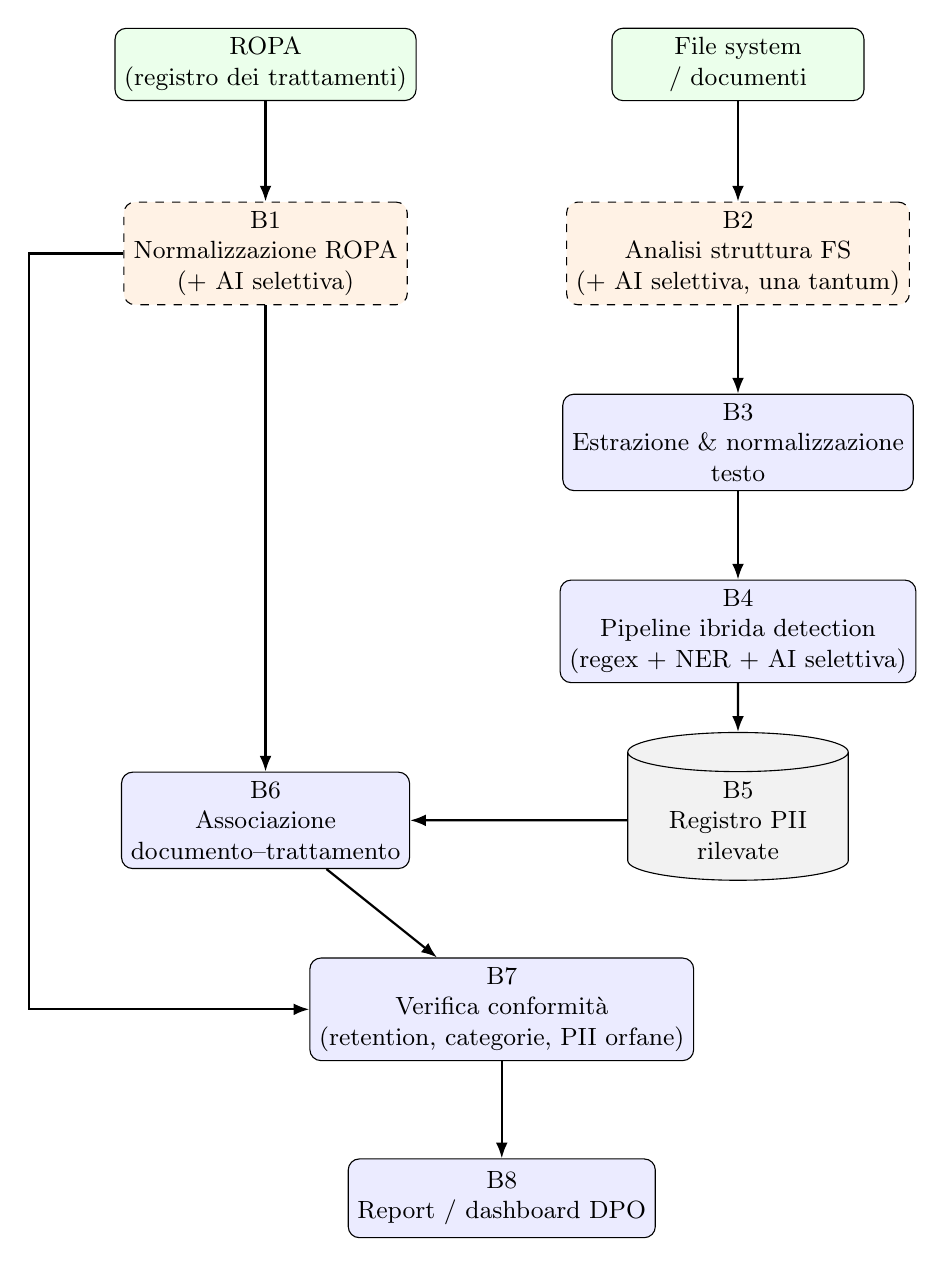
\begin{tikzpicture}[
			block/.style={rectangle, draw, rounded corners, minimum width=3.6cm,
					minimum height=1cm, align=center, fill=blue!8, font=\small},
			onetime/.style={rectangle, draw, dashed, rounded corners, minimum width=3.6cm,
					minimum height=1cm, align=center, fill=orange!10, font=\small},
			store/.style={cylinder, draw, shape border rotate=90, aspect=0.25,
					minimum height=1.6cm, minimum width=2.8cm, align=center, fill=gray!10, font=\small},
			input/.style={rectangle, draw, rounded corners, minimum width=3.2cm,
					minimum height=0.9cm, align=center, fill=green!8, font=\small},
			arrow/.style={thick, -{Latex[length=2mm]}},
		]

		% --- Input (riga y=0) ---
		\node (ropa) [input] at (0,0)   {ROPA\\(registro dei trattamenti)};
		\node (fs)   [input] at (6,0)   {File system\\/ documenti};

		% --- Blocchi una tantum (riga y=-2.4) ---
		\node (b1) [onetime] at (0,-2.4) {B1\\Normalizzazione ROPA\\(+ AI selettiva)};
		\node (b2) [onetime] at (6,-2.4) {B2\\Analisi struttura FS\\(+ AI selettiva, una tantum)};

		% --- Pipeline ricorrente (colonna destra, righe successive) ---
		\node (b3) [block] at (6,-4.8) {B3\\Estrazione \& normalizzazione\\testo};
		\node (b4) [block] at (6,-7.2) {B4\\Pipeline ibrida detection\\(regex + NER + AI selettiva)};

		% --- Persistenza / associazione (riga y=-9.6) ---
		\node (b6) [block] at (0,-9.6) {B6\\Associazione\\documento--trattamento};
		\node (b5) [store] at (6,-9.6) {B5\\Registro PII\\rilevate};

		% --- Conformità e output ---
		\node (b7) [block] at (3,-12.0)  {B7\\Verifica conformità\\(retention, categorie, PII orfane)};
		\node (b8) [block] at (3,-14.4)  {B8\\Report / dashboard DPO};

		% --- Frecce: pipeline principale ---
		\draw [arrow] (ropa) -- (b1);
		\draw [arrow] (fs)   -- (b2);
		\draw [arrow] (b2)   -- (b3);
		\draw [arrow] (b3)   -- (b4);
		\draw [arrow] (b4)   -- (b5);
		\draw [arrow] (b5)   -- (b6);
		\draw [arrow] (b6)   -- (b7);
		\draw [arrow] (b7)   -- (b8);

		% --- Freccia B1 -> B6 (verticale, colonna libera) ---
		\draw [arrow] (b1) -- (b6);

		% --- Freccia B1 -> B7: corsia dedicata a sinistra, niente clipping ---
		\draw [arrow] (b1.west) -- ++(-1.2,0) |- (b7.west);

	\end{tikzpicture}
	\caption{Architettura a macro-blocchi del sistema}
	\label{fig:architettura-macro-blocchi}
\end{figure}

\begin{figure}[htbp]
	\centering
	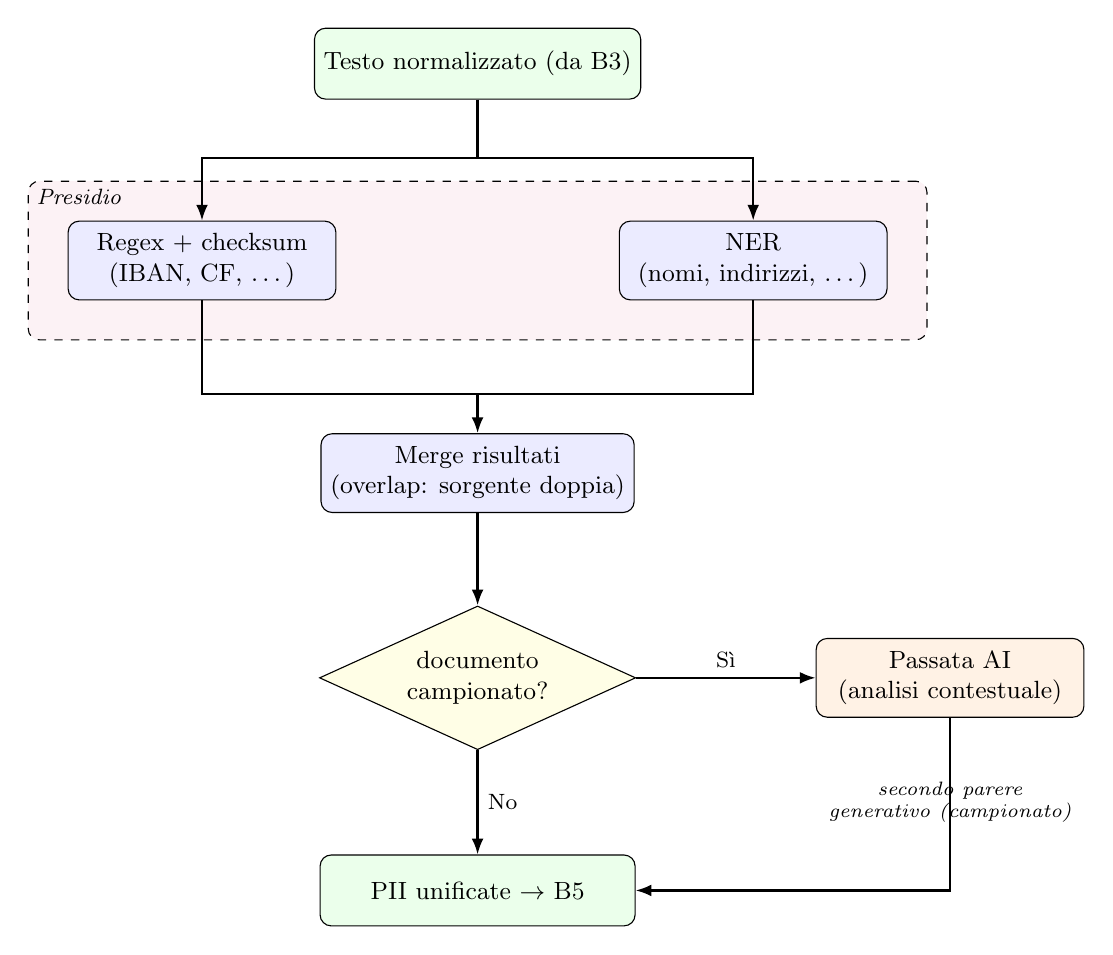
\begin{tikzpicture}[
			block/.style={rectangle, draw, rounded corners, minimum width=3.4cm,
					minimum height=1cm, align=center, fill=blue!8, font=\small},
			decision/.style={diamond, draw, minimum width=3cm, minimum height=1.2cm,
					align=center, fill=yellow!10, font=\small, aspect=2.2},
			ai/.style={rectangle, draw, rounded corners, minimum width=3.4cm,
					minimum height=1cm, align=center, fill=orange!10, font=\small},
			io/.style={rectangle, draw, rounded corners, minimum width=4cm,
					minimum height=0.9cm, align=center, fill=green!8, font=\small},
			arrow/.style={thick, -{Latex[length=2mm]}},
		]

		% --- Nodi ---
		\node (input)   [io]       at (0,    0)    {Testo normalizzato (da B3)};
		\node (regex)   [block]    at (-3.5, -2.5) {Regex + checksum\\(IBAN, CF, \ldots)};
		\node (ner)     [block]    at ( 3.5, -2.5) {NER\\(nomi, indirizzi, \ldots)};
		\node (merge)   [block]    at (0,    -5.2) {Merge risultati\\(overlap: sorgente doppia)};
		\node (counter) [decision] at (0,    -7.8) {documento\\campionato?};
		\node (ai)      [ai]       at (6,    -7.8) {Passata AI\\(analisi contestuale)};
		\node [font=\scriptsize\itshape, align=center, anchor=north] at (6, -9.0)
		{secondo parere\\generativo (campionato)};
		\node (output)  [io]       at (0,   -10.5) {PII unificate $\rightarrow$ B5};

		% --- Motore Presidio: fornisce i detector regex e NER (merge/AI restano proprietari) ---
		\begin{scope}[on background layer]
			\node (presidio) [draw, dashed, rounded corners, fill=purple!5,
				inner sep=5mm, fit=(regex)(ner)] {};
		\end{scope}
		\node [font=\footnotesize\itshape, anchor=north west, inner sep=3pt]
		at (presidio.north west) {Presidio};

		% --- Fork: input -> regex + ner (parallelo) ---
		\coordinate (fk) at (0, -1.2);
		\draw [thick] (input.south) -- (fk);
		\draw [arrow] (fk) -| (regex.north);
		\draw [arrow] (fk) -| (ner.north);

		% --- Join: regex + ner -> merge ---
		\coordinate (jn) at (0, -4.2);
		\draw [thick] (regex.south) |- (jn);
		\draw [thick] (ner.south)   |- (jn);
		\draw [arrow] (jn) -- (merge.north);

		% --- Merge -> counter ---
		\draw [arrow] (merge.south) -- (counter.north);

		% --- Counter: No -> output ---
		\draw [arrow] (counter.south) -- node[right, font=\footnotesize]{No} (output.north);

		% --- Counter: Sì -> AI ---
		\draw [arrow] (counter.east) -- node[above, font=\footnotesize]{Sì} (ai.west);

		% --- AI -> output ---
		\draw [arrow] (ai.south) |- (output.east);

	\end{tikzpicture}
	\caption[Dettaglio del blocco B4: pipeline ibrida di rilevamento PII]{Dettaglio del blocco B4: pipeline ibrida di rilevamento PII. I detector regex e NER sono forniti da Presidio (\texttt{AnalyzerEngine}) dietro il contratto \texttt{PIIDetector}; il merge resta proprietario. Il ramo in basso a destra --- il campionamento e la passata AI contestuale --- è \emph{realizzato}: su un campione di documenti un rilevatore generativo produce candidati che entrano nel merge come terza sorgente, confermando o scoprendo PII (§\ref{sub:b4-ai-previsto}). Lo schema è una semplificazione di flusso: i candidati generativi confluiscono nel merge accanto a quelli di regex e NER, non a valle di esso.}
	\label{fig:b4-detection-pipeline}
\end{figure}

% Le figure d'apertura del capitolo restano confinate qui, prima delle sezioni.
\FloatBarrier

La figura \ref{fig:architettura-macro-blocchi} rappresenta graficamente l'intero sistema, e costituisce la ground truth per quanto riguarda la sua implementazione. I seguenti capitoli sono suddivisi seguendo rigorosamente i blocchi dell'architettura prevista dal grafico.

\section{Input del sistema}
\label{sec:input-sistema}

Prima di discutere dei componenti attivamente presenti nel sistema, è importante inquadrare quali sono gli input usati dal sistema all'inizio della pipeline di esecuzione.

\subsection{ROPA - Registro dei Trattamenti}
\label{sub:input-ROPA}
Il primo input è il \textit{Registro dei Trattamenti (ROPA)} di un'azienda. In generale, non esiste un template riconosciuto universalmente. Questa disomogeneità porta la sua complessità, per una serie di motivi:
\begin{itemize}
	\item Tipo di file: essendo un tipo di dato libero, la sua interpretazione e decisione su come salvarlo ricade sull'azienda in questione. Esistono centinaia di modi diversi per salvare un registro, ognuno dei quali richiede particolare attenzione.
	\item Sintassi di scrittura: seppur inquadrando un certo tipo di file come più adatto, è comunque difficile predirre esattamente dove il dato a noi importante (le categorie salvate, per esempio), si trovarà all'interno del file. Questa caratteristica implica l'introduzione di un tipo di complessità basata sul contesto, ambito in cui gli algoritmi tradizionali peccano in efficienza. Una strada è sicuramente l'uso di AI generativa per la comprensione completa del documento in questione e il suo adattamento. Tuttavia, questo porta numerosi problemi, che inoltre, trascendono dallo scope di questo lavoro (AI generativa per parsing dei parametri, giusto per leggere leggermente meglio un documento)
\end{itemize}

\subsection{File system}
\label{sub:input-FS}
Il secondo input del sistema rappresenta l'insieme dei file che vanno analizzati dal sistema stesso. È possibile decidere di analizzare un singolo file, oppure un'intera cartella, o più in linea con lo scope del progetto, un'intero insieme di sottocartelle, essendo che la cartella selezionata all'interno del file system rappresenta la root da cui far partire la scansione. Per semplicità, e per bacino di utenza, è stato deciso di supportare solo un sottoinsieme di tipologie di file, includendo i più utilizzati sia in ambito consumer che enterprise. Questa scelta è stata ponderata sul fatto che, garantire il supporto ad un'infinità di tipi di file, è sicuramente un'ottima feature, ma poco interessante e poco inerente con lo scope di questo lavoro. Di conseguenza, è sembrato più consono garantire il supporto ai tipi di file "scontati" quando ci si riferisce a \textit{file non strutturati}.










\section{B1 - Normalizzazione ROPA}
\label{sec:b1-ropa}
Questo blocco è responsabile per la lettura e trasformazione del registro dei trattamenti in una forma standardizzata del sistema. Questo passaggio è obbligatorio, in quanto il termine di paragone per la verifica di conformità è tra il Registro dei Trattamenti e le PII identificate nei documenti: senza una struttura fissa e standardizzata, un confronto sarebbe estremamente dispendioso e complesso.

È stata effettauta una scelta ponderata per quanto riguarda lo schema della struttura dati che avrebbe contenuto i ROPA. Si sono presentate due possibili strade:
\begin{itemize}
	\item Struttura dati definita a monte: viene imposto uno schema noto e il database viene popolato in maniera deterministica partendo dal ROPA in input.
	\item Struttura scelta da un agente di intelligenza artificiale: il ROPA viene fornito al modello, delegando a lui la creazione della struttura del database, in base al contesto e a ciò che reputa migliore per il salvataggio in maniera efficiente dei dati.
\end{itemize}
È stata adottata la prima opzione per il seguente motivo: un Registro dei trattamento è un documento di conformità \textbf{legale}. Bisogna predilire affidabilità e riproducibilità nella sua creazione. Un modello di AI, seppur potenzialmente in grado di fornire informazioni aggiuntive, può essere soggetto ad allucinazioni o a risultati non riproducibili, casistiche non tollerabili per questi contesti.

Avere uno schema esplicito garantisce che il database sia interrogabile in maniera prevedibile dal blocco di confronto B7 (\ref{sec:b7-verifica-compliance-PII}) e mantenibile nel tempo.

L'AI non viene esclusa, ma spostata in un ambito più creativo durante la creazione del database del registro dei trattamenti (\ref{DA METTERE}).

\subsection{Template registro CNIL}
\label{sub:B1-cnil}
Per fronteggiare al problema dell'inesistenza di un template universalmente condiviso a livello mondiale o europeo per i Registri dei Trattamenti, è stato deciso di adottare come template supportato quello fornito dalla \textit{Commission Nationale de l'Informatique et des Libertés (CNIL)}, autorità di controllo francese che mette a disposizione online una versione basilare ma completa, per aiutare le azienda ad orientarsi nella creazione del proprio registro ~\cite{cnilRegistreTraitement, cnilRegistreModeleBasique}.

Questo modello è organizzato per attività di trattamento: un foglio Excel per ogni trattamento, con i seguenti campi.
\begin{itemize}
	\item identificazione del trattamento (nome, date di creazione e aggiornamento, base giuridica);
	\item attori: titolare del trattamento, eventuali co-titolari, responsabile della protezione dei dati (DPO), responsabili del trattamento esterni (\textit{processors});
	\item finalità del trattamento;
	\item categorie di persone interessate;
	\item categorie di dati personali, con evidenziazione delle categorie particolari (dati sensibili);
	\item categorie di destinatari (interni, esterni, responsabili esterni);
	\item trasferimenti verso Paesi terzi (destinazione e garanzie);
	\item durate di conservazione;
	\item misure di sicurezza tecniche e organizzative.
\end{itemize}

Per lo scopo del lavoro, \textbf{non verranno salvati tutti i dati} presenti in un trattamento. Questa scelta è stata fatta per ridurre la complessità ed evitare di salvare dati potenzialmente sensibili all'interno del database del sistema, senza un vero e proprio scopo. Di conseguenza, gli unici dati che sistematicamente vengono salvati sono quelli presenti nelle sezioni:
\begin{itemize}
	\item identità del trattamento;
	\item categorie di dati personali.
\end{itemize}

% qui da valutare se mettere la discussione con relatore
La struttura scelta per rappresentare il registro segue la sua gerarchia naturale su \textbf{tre livelli}. Al primo, l'\textbf{attività di trattamento}, con la sua identità (un nome e una finalità). Al secondo, i \textbf{blocchi di categorie} che vi appartengono, ciascuno con la propria \textbf{durata di conservazione}, che le categorie raccolte nel blocco ereditano. Al terzo, le \textbf{singole categorie dichiarate}, ognuna ricondotta al vocabolario condiviso delle categorie di PII --- lo stesso usato dal rilevamento (B4). È quest'ultimo aggancio a rendere il confronto fra ciò che il registro \emph{dichiara} e ciò che il motore \emph{rileva} (B7) una semplice operazione insiemistica: e una categoria che non si risolve in alcun tipo rilevabile resta \textbf{esplicita} nel modello --- dichiarata ma non verificabile dal motore --- e come tale va segnalata al DPO, non scambiata per conforme. La durata di conservazione, infine, è tenuta accanto al testo originale in forma \emph{confrontabile dalla macchina}, così che il superamento del termine (B7) sia \emph{calcolato} al momento del controllo e non registrato come stato. La resa concreta di questo modello --- tabelle, campi e tipi --- è nella sezione di implementazione (§\ref{sec:dati-persistiti}).


\subsection{Ruolo AI in ROPA}
\label{sub:B1-AI}

Il popolamento dei primi due livelli del modello --- l'attività di trattamento e i blocchi di categorie --- è deterministico: la struttura CNIL è nota e i campi si trasferiscono direttamente. Il terzo livello, la singola categoria dichiarata, è invece spesso testo libero e sbrigativo («dati anagrafici, coordinate bancarie, contatti»): ricondurlo al \textbf{vocabolario condiviso delle categorie di PII} --- lo stesso che il rilevamento (B4) usa --- richiede un'interpretazione contestuale, per la quale un algoritmo puramente sintattico è inadeguato. È l'unico punto dell'ingestione in cui interviene un modello generativo, ed entro due vincoli architetturali stretti. Primo, è un intervento \textbf{circoscritto}: una volta, a livello di singolo campo, per scindere ed espandere un testo libero in categorie normalizzate --- non una delega della struttura del documento, coerente con la scelta \emph{non agentica} del blocco. Secondo, opera dentro un \textbf{vocabolario chiuso}: ogni categoria proposta è validata contro quel catalogo condiviso, e una proposta che non vi rientra è scartata, sicché il modello non può introdurre categorie che il sistema non sa rilevare.

Soprattutto, l'esito del modello è una \emph{proposta}, non una decisione: la mappatura resta tale finché il DPO non la conferma. È l'istanza, in questo blocco, di un principio che attraversa l'intero sistema: qualunque sia l'origine di un'inferenza --- un dizionario deterministico, un modello generativo, una regola che associa una cartella a un trattamento, la segnalazione di una PII orfana --- l'atto che la rende parte della \emph{verità dichiarativa} è sempre umano. Il sistema propone, il DPO dispone. È il gemello, sul versante della decisione, dei principi di \emph{recall-first} e di \emph{minimizzazione}: come quelli evitano rispettivamente di scartare e di trattenere, questo evita di \textbf{decidere al posto dell'umano}. La realizzazione --- i due mapper intercambiabili, il prompt, la validazione, la conferma --- è descritta in §\ref{sub:impl-b1-mappatura}.
















% ============================================================================
% SCAFFOLDING (temporaneo) — mappa parallela §6 (idea) <-> §7 (realizzazione).
% Struttura dati DENTRO i blocchi. In §6 il lavoro e' quasi tutto RECUPERO dalle
% vecchie sezioni tematiche piu' in basso (237+): svuotarle in questi stub e poi
% cancellarle. Eliminare questo scaffold a lavoro finito.
% ----------------------------------------------------------------------------
% B2 - Analisi struttura FS (NON realizzato)
%   §6: perche' previsto e non fatto (l'utile e' gia' dato dalle regole
%       cartella->trattamento, B6). Recuperare da: §"Un blocco previsto e non
%       realizzato" (piu' in basso).  |  §7: nulla (non implementato).
% ----------------------------------------------------------------------------
% B3 - Estrazione e normalizzazione del testo
%   §6 (idea): estrazione born-digital -> testo normalizzato; la DATA DI
%       RIFERIMENTO con provenienza (metadati->mtime) come dato del blocco;
%       niente OCR/layout. Recuperare da: §"Livello di estrazione del testo".
%   §7 (come): lettori PDF/DOCX/txt + fogli + .doc legacy; extraction/dates.py
%       (catena metadati->mtime, guardia <1990/futuro, degrado grazioso).
%   struttura inline (§6): il documento normalizzato + reference_date con la fonte.
% ----------------------------------------------------------------------------
% B4 - Pipeline ibrida di detection
%   §6 (idea): due sorgenti dietro PIIDetector + il merge (4 casi) + il ramo
%       generativo. GIA' SCRITTO piu' in basso (§"Livello di rilevamento ibrido":
%       sorgenti / merge / ramo AI) -> SPOSTARE qui.
%   §7 (come): Presidio pattern+NER, GLiNER, RegexDetector config-driven (gia' in
%       §7), LLMDetector (prompt, valore->span, chunking, never-raise), MergeEngine,
%       slot opzionale ai + AITriggerPolicy.
%   struttura inline: PIICandidate -> PIIMatch (span, tipo, confidence, livello, sorgenti).
% ----------------------------------------------------------------------------
% B5 - Registro PII rilevate
%   §6 (idea): changelog delta-based (stato + storia); i DUE OROLOGI (data
%       semantica vs impronta tecnica); minimizzazione (mai il valore).
%       Recuperare da: §"Persistenza del registro delle PII".
%   §7 (come): 4 tabelle (document/scan/instance/change); freshness (incrementale);
%       refresh CONFIRMED. GIA' in §7 (§"Dati persistiti" -> registro PII).
%   struttura inline (§6): documento -> scansione -> istanza (stato) + variazione (log); ER concettuale.
% ----------------------------------------------------------------------------
% B6 - Associazione documento-trattamento
%   §6 (idea): associazione esplicita + regole cartella (prefisso->attivita'),
%       provenienza MANUAL/RULE; + IL PONTE CROSS-DB: due database separati, join
%       LOGICO sull'id-stringa (QUI il posto giusto per il pezzo trasversale).
%       Recuperare da: §"Associazione e verifica" -> sottosez. B6.
%   §7 (come): FolderRule, riconciliazione (azzera RULE stale), auto-apply a fine scan.
%   struttura inline: Document.activity_ids (N:N) + FolderRule(prefix->activity_ids).
% ----------------------------------------------------------------------------
% B7 - Verifica conformita' + conservazione
%   §6 (idea): confronto should/is -> orfane/coperte/mancanti; retention (eta' vs
%       termine + "non verificabile"); + DALLA PII ORFANA ALLA PROPOSTA (il
%       feedback: orphan -> categoria PROPOSED, il DPO conferma). Recuperare da:
%       §"Associazione e verifica" -> sottosez. B7 + "Verifica della conservazione".
%   §7 (come): checker.build_report; vista di corpus /retention; propose_category.
%   struttura inline (§6): il verdetto (ComplianceReport) come valore di sola lettura.
% ----------------------------------------------------------------------------
% B8 - Dashboard DPO
%   §6 (idea): restituzione al DPO; human-in-the-loop (gia' enunciato in B1);
%       Post/Redirect/Get come principio. Recuperare da: §"Interfaccia e
%       restituzione al DPO".
%   §7 (come): app FastAPI unica (una porta); pagine (dashboard / documento /
%       /retention / /scan / /rules; review ROPA montata sotto /ropa); trigger AI
%       (menu campionamento, per-documento ASINCRONO via ScanJob); due fasi;
%       indicatore di scansione attiva.
% ----------------------------------------------------------------------------
% TRASVERSALE
%   §6: nuova sezione "Pattern architetturali e di progettazione" (Strategy / DI /
%       Factory / Adapter / Composite / Policy / Active Record; l'argomento
%       Open-Closed che giustifica lo slot opzionale invece di un Registry = YAGNI).
%   §7: "Deployment containerizzato" (GIA' SCRITTO).
%   Principi trasversali, enunciati UNA volta: recall-first, minimizzazione, DPO
%   sovrano (gia' in B1).
% ============================================================================

\section{B2 - Analisi struttura File System}
\label{sec:b2-analisi-struttura}
Feature presente nell'architettura originale, ma non implementata per vincoli tempistici e di scarsa sicurezza e utilità del possibile risultato. Presente in maniera più approfondita nella sezione degli Sviluppi Futuri \ref{SEZIONE}

\section{B3 - Estrazione e normalizzazione del testo}
\label{sec:b3-estrazione-testo}

Il blocco B3 sta a monte del rilevamento: trasforma un file, in uno dei formati supportati (§\ref{sub:input-FS}), nel \textbf{testo normalizzato} su cui opererà il motore di detection. Il suo prodotto è deliberatamente semplice --- un flusso di testo lineare, spogliato della formattazione --- ed è \emph{questo}, non il documento originale, ciò che entra nel blocco B4: la medesima forma di testo è consumata allo stesso modo dai rilevatori a regole e dal modello generativo, sicché a valle nessuno deve più sapere da quale formato il documento provenisse. La normalizzazione è leggera (spazi e a-capo) e non tenta di ricostruire il \emph{layout}: il sistema tratta documenti \emph{born-digital}, non scansioni, e l'OCR resta fuori ambito (cfr.~§\ref{cap:sviluppi-futuri}).

Una scelta di progetto merita di essere resa esplicita, perché ribalta un'assunzione iniziale. L'estrazione era stata concepita attorno a uno strumento dedicato --- Docling~\cite{livathinosDoclingEfficientOpenSource2025} --- pensato per convertire formati complessi in testo pulito, fruibile tanto da un modello generativo quanto dai rilevatori a regole. All'atto dell'implementazione, però, i formati che selezionati per essere supportati si sono rivelati sufficentemente semplici da non richiedere quell'apparato: bastano conversioni leggere che riducono ogni file a un flusso di testo direttamente analizzabile. Docling resta possibile risorsa qualora l'insieme dei formati si allargasse a documenti realmente complessi (§\ref{cap:sviluppi-futuri}); allo stato attuale sarebbe complessità non ripagata. Coerentemente con la separazione fra architettura e realizzazione, le scelte implementative appartengono al capitolo di implementazione (§\ref{sec:impl-b3-estrazione}).

% ---------------------------------------------------------------------------
% Bozza mista originale (NON cancellare --- traccia da cui e' derivato il testo sopra
% e le indicazioni §6/§7; da rimuovere a lavoro finito):
% Questa registrazione serve come in base per poi scrivere il la sezione B3 per quanto riguarda l'estrazione, la normalizzazione del testo dei documenti del sistema. Questa sezione in particolare inizialmente era stata pensata per essere. Soltanto basata su dockling Una applicazione. esterna che Il suo compito è quello di convertire formati particolarmente. Complessi in testo facilmente leggibile sia da AI, ma anche da rilevatori Basati su regole come presidio, quello che viene usato nel progetto, d'altronde. Dopo però L'inizio dell'implementazione La cosa è stata più semplice del previsto in quanto i tipi di file. Che ho deciso di trattare Erano molto più primitivi di quello che mi aspettassi. Infatti. È bastato utilizzare delle librerie in Python molto più leggere e che permettevano. Di trasformare al volo il file in questione direttamente diciamo. In una streaming di testo che poteva essere molto più facilmente. Parsata dal Dal motore di rilevamento. I tipi di file supportati. Sono quelli più utilizzati a livello enterprise, a livello customer. Ma questa sezione c'è già precedentemente. sui tipi di file appunto supportati nella sezione del file system. Nella in questa sezione di architettura. Non vanno messi i nomi delle librerie in sé andranno messi poi nella sicuramente nella sezione di implementazione con anche tipo di tipo di estensione del file con. Il nome della libreria e il suo eventuale utilizzo, ovviamente senza entrare eccessivamente nel dettaglio, ma comunque è giusto. Dirlo. Quindi questo è per quanto riguarda il blocco B3. Cosa da mettere secondo me che ha senso in questa sezione qual è l'effettivo. Output di questo blocco o meglio che cosa entra direttamente nel blocco B4 della detection. Secondo me, appunto centrale. Però iniziamo a scrivere questo
% ---------------------------------------------------------------------------

\section{B4 - Pipeline ibrida di detection di PII}
\label{sec:b4-pipeline-detection}
\label{sec:rilevamento-b4}

Il blocco B4 della Figura~\ref{fig:architettura-macro-blocchi} è il motore di rilevamento vero e proprio: dato il testo già estratto e normalizzato dal blocco a monte, individua le PII presenti nel documento e le consegna, unificate, al registro (B5). È un livello \emph{ibrido}, che combina due tecniche indipendenti e complementari --- un'impostazione che la letteratura recente sul rilevamento di PII indica come la più robusta rispetto alle singole tecniche prese isolatamente~\cite{mishraHybridRulebasedNLP2025, rajgarhiaEvaluationStudyHybrid2025}; la sua architettura interna è dettagliata nella Figura~\ref{fig:b4-detection-pipeline}.

\subsection{Due sorgenti complementari dietro un contratto unico}
\label{sub:b4-sorgenti}

Le due tecniche coprono classi di PII diverse. Le \textbf{espressioni regolari}, affiancate dalla verifica di \emph{checksum} dove il formato la prevede, riconoscono gli \emph{identificatori strutturati} --- IBAN, codice fiscale, numero di carta, indirizzo IP --- dove la forma è rigida e la precisione può essere massima. Il \textbf{riconoscimento di entità nominate} (NER) copre invece i dati meno strutturati e dipendenti dal contesto --- nomi di persona, indirizzi --- dove nessuna regola fissa è sufficiente. La validazione a \emph{checksum} non è un affinamento previsto ma una proprietà già operante: un IBAN o un codice fiscale formalmente ben scritto ma incoerente nella cifra di controllo viene scartato, ed è la ragione per cui il corpus di valutazione (Cap.~\ref{cap:test}) deve generare valori \emph{aritmeticamente validi} --- altrimenti sarebbe il \emph{gold} stesso a essere respinto, gonfiando artificiosamente i falsi negativi.

Entrambe le tecniche sono esposte al resto del sistema attraverso un unico contratto, \texttt{PIIDetector} (nella forma \texttt{detect(testo)} $\rightarrow$ lista di candidati): l'orchestrazione dipende solo da questa forma, non dalla tecnologia sottostante, così una sorgente può essere sostituita senza toccare il resto del livello. Nella realizzazione le due sorgenti poggiano sul motore \textit{open source} Microsoft Presidio~\cite{HomeMicrosoftPresidio}, adottato come base per regex e NER a valle di una valutazione sperimentale (§\ref{sec:valutazione-presidio}).

\paragraph{Estendere il rilevamento senza scrivere codice.} Lo stesso contratto rende possibile \emph{comporre} più rilevatori in un unico posto della pipeline. Su questa possibilità poggia il punto di estensione richiesto dai requisiti (cfr.~§\ref{sub:estensibilita}): accanto ai riconoscitori predefiniti opera un rilevatore \textbf{guidato da configurazione}, che esegue le regole dichiarate in un file esterno. Aggiungere un identificatore proprio di un settore o di un ordinamento --- e la categoria corrispondente nel catalogo --- è quindi una modifica \emph{dichiarativa}, non un intervento sul codice sorgente. La coerenza di questa scelta è stata verificata applicandola a sé stessa: l'unico identificatore che era stato cablato nel motore come caso speciale (il numero AVS svizzero) è stato ricondotto al medesimo meccanismo, così che esista una sola strada per tutti i pattern anziché due.

\subsection{Il merge: unificazione e grado di certezza}
\label{sub:b4-merge}

Le due sorgenti producono candidati in modo autonomo; il \emph{merge} li unifica in un unico insieme di PII, decidendone il grado di certezza in base a \emph{quante} e \emph{quali} sorgenti concordano su una stessa porzione di testo. Confrontando gli span per sovrapposizione, ogni PII risultante ricade in uno di quattro casi --- un vocabolario chiuso:

\begin{itemize}
	\item \textbf{Fonte singola} --- rilevata da una sola tecnica, senza sovrapposizioni. Non viene mai scartata (cfr.\ il principio \emph{recall-first} più sotto), ma etichettata come meno certa.
	\item \textbf{Doppia conferma} --- due o più sorgenti concordano sullo stesso tipo di PII su span sovrapposti: pattern e NER, oppure l'una o l'altra insieme alla passata generativa. È il caso più solido: la confidenza viene rinforzata.
	\item \textbf{Conflitto} --- gli span si sovrappongono ma le sorgenti assegnano tipi diversi. Il merge \textbf{non arbitra}: conserva entrambe le ipotesi e demanda la risoluzione al blocco a valle, che dispone di più contesto.
	\item \textbf{Scoperta dall'AI} --- individuata dalla passata generativa selettiva (campionata), assente dalle altre sorgenti. È il caso in cui il modello generativo aggiunge qualcosa che gli algoritmi tradizionali non hanno visto (§\ref{sub:b4-ai-previsto}).
\end{itemize}

\paragraph{Principio recall-first.} Nessuna sorgente scarta di propria iniziativa un candidato debole: al più lo segnala con confidenza bassa. La ragione è la finalità di conformità del sistema: un falso positivo costa al DPO una verifica in più, mentre una PII \emph{mancata} è un rischio che resta invisibile. Il merge eredita questo principio --- non elimina, ma unifica e classifica --- lasciando ogni eventuale scarto a una decisione umana o a un blocco a valle.

\paragraph{Il ruolo della passata generativa.} La terza sorgente, quando presente, entra nel merge per ultima e vi gioca due ruoli. Se ricade su una PII già trovata e ne concorda il tipo è \emph{confermatrice}: la sua provenienza si aggiunge alle altre e la certezza sale (una fonte singola diventa a doppia conferma, una già doppia acquista una terza voce). Se cade dove nessun'altra sorgente ha visto nulla è \emph{scopritrice}, e produce il quarto caso. Il disaccordo segue lo stesso principio recall-first, ma pesato: un parere generativo singolo che contraddice un'altra fonte mette le due sullo stesso piano (entrambe in conflitto, arbitraggio a valle), ma \textbf{non basta a incrinare} un accordo già raggiunto fra pattern e NER, che resta tale. La certezza, in altre parole, non si perde per una contestazione più debole di ciò che contesta.

\paragraph{Un solo modello dato.} La PII unificata prodotta dal merge non richiede un modello dati intermedio: la sua \emph{certezza} è già descritta da tre attributi che essa porta con sé --- la confidenza (quanto è forte il rilevamento), il livello di conferma appena descritto, e l'elenco delle \emph{provenienze} (quali e quanti detector concordano, ciascuno con la propria confidenza). Mantenere questi campi sul singolo oggetto, invece di duplicarli in strutture parallele, conserva un'unica fonte di verità per la PII rilevata e ne preserva la tracciabilità verso il DPO.

\subsection{Il ramo generativo come secondo parere}
\label{sub:b4-ai-previsto}

Le due sorgenti descritte finora appartengono al paradigma degli algoritmi \emph{tradizionali}: veloci, deterministici, economici, ma ciechi a tutto ciò che non è previsto in una regola o in un'etichetta. Il ramo generativo affianca loro un modello linguistico come \emph{secondo parere}, per rispondere a una domanda che è di merito e non di ingegneria --- se e quando un modello che legge il documento come farebbe un lettore umano~\cite{brownLanguageModelsAre2020} trovi dato personale che quegli algoritmi non trovano, e se il guadagno giustifichi il suo costo, superiore di ordini di grandezza in tempo ed energia. La scelta del modello e la sua valutazione sono l'oggetto degli studi che precedono la progettazione (§\ref{sec:scelta-modello-llm}, distinzione Task 1 / Task 2 in §\ref{sub:slm-task}); l'esito comparativo è nel Capitolo~\ref{cap:risultati}.

Ciò che qui rileva è la forma architetturale, ed è dettata proprio da quella domanda: perché l'AI sia \emph{confrontabile} con le sorgenti tradizionali, va costruita come una sorgente fra le altre, non come un meccanismo a parte. Il rilevatore generativo è perciò incapsulato dietro lo stesso contratto \texttt{PIIDetector} di regex e NER, così che il merge lo accolga come terza voce (§\ref{sub:b4-merge}) e lo stesso apparato di misura che assegna precisione e richiamo a un rilevatore possa assegnarli al modello generativo senza codice speciale.

\paragraph{Quando accendere l'AI: una politica del chiamante.} Una passata generativa costa da secondi a minuti per documento, quindi non la si esegue su ogni file a ogni scansione (cfr.\ l'impiego \emph{selettivo} previsto dai requisiti, §\ref{sub:ai-selettiva}, e il costo in §\ref{sec:impatto-ambientale}). La decisione su \emph{quali} documenti sottoporre all'AI è però tenuta \textbf{fuori} dal rilevatore --- che si limita ad analizzare il testo che riceve --- e affidata a una \emph{politica} del chiamante: nessuna analisi, tutti i documenti, oppure un campione. Separare la politica dal rilevatore è ciò che consente di innescare l'AI in modi diversi (a campione durante una scansione, o su richiesta su un singolo documento) senza duplicare la logica di rilevamento. La realizzazione del rilevatore e della politica --- prompt a catalogo chiuso, difese anti-allucinazione, campionamento --- è descritta in §\ref{sec:impl-detection}.

\section{B5 - Registro PII rilevate}
\label{sec:b5-DB-PII}

\section{B6 - Associazione documento-trattamento}
\label{sec:b6-documento-trattamento}

\section{B7 - Verifica conformità PII presenti}
\label{sec:b7-verifica-compliance-PII}

\section{B8 - Dashboard per DPO}
\label{sec:b8-dashboard}

\section{Ingestione e modello dati del ROPA}
\label{sec:modello-ropa}

Il blocco B1 della Figura~\ref{fig:architettura-macro-blocchi} acquisisce il ROPA (\textit{Record of Processing Activities}, il registro delle attività di trattamento) e lo trasforma in una rappresentazione interna. Non è una fase accessoria: il ROPA è il termine di paragone \textit{atteso} rispetto al quale la verifica di conformità (B7) confronta le PII effettivamente rilevate nei documenti. La sua struttura dati condiziona quindi ciò che il sistema è in grado di verificare. Questa sezione motiva l'approccio scelto per modellarlo.

\subsection{Strutturazione a monte o delega all'AI}
\label{sub:ropa-approccio}

L'ingestione del ROPA ammette due strategie agli estremi opposti. Nella prima la \textbf{struttura dati è definita a monte}: il sistema impone uno schema noto e l'ingestione lo popola in modo deterministico a partire da un ROPA già compilato. Nella seconda, \textbf{totalmente agentica}, i documenti del ROPA vengono forniti così come sono a un modello generativo, delegando a esso l'individuazione della struttura --- l'approccio «si immettono i documenti e si osserva cosa emerge».

Si adotta la prima. Un registro dei trattamenti è un \textit{artefatto di conformità}: la sua affidabilità e la sua auditabilità non possono dipendere da una strutturazione inferita, potenzialmente allucinata e non riproducibile. Uno schema esplicito garantisce inoltre che il modello sia interrogabile in modo prevedibile dal blocco di confronto (B7) e mantenibile nel tempo. L'AI non viene esclusa, ma \textbf{circoscritta} a un ruolo di arricchimento su un singolo campo (§\ref{sub:ropa-ai}); ciò è coerente con l'uso selettivo dell'AI già previsto per il blocco B1 nella Figura~\ref{fig:architettura-macro-blocchi}.

\subsection{Il registro-tipo CNIL come schema di riferimento}
\label{sub:ropa-cnil}

Il contenuto obbligatorio del registro è fissato dall'art.~30 del Regolamento (UE) 2016/679~\cite{gdprArt30} e, per il contesto svizzero, dall'art.~12 della LPD~\cite{nlpdArt12}; i due elenchi sono ampiamente sovrapponibili. In assenza di una pluralità di modelli operativi consolidati, il riferimento pratico più diffuso è il registro-tipo pubblicato dalla \textit{Commission Nationale de l'Informatique et des Libertés} (CNIL), l'autorità di controllo francese, derivato direttamente dall'art.~30~\cite{cnilRegistreTraitement, cnilRegistreModeleBasique}. Adottarlo come base evita di progettare uno schema dal principio e lega il modello ad una fonte ampiamente autorevole e condivisa.

Il modello CNIL è organizzato per \textit{attività di trattamento}: una scheda per ciascun trattamento, con i campi seguenti.
\begin{itemize}
	\item identificazione del trattamento (nome, date di creazione e aggiornamento, base giuridica);
	\item attori: titolare del trattamento, eventuali co-titolari, responsabile della protezione dei dati (DPO), responsabili del trattamento esterni (\textit{processors});
	\item finalità del trattamento;
	\item categorie di persone interessate;
	\item categorie di dati personali, con evidenziazione delle categorie particolari (dati sensibili);
	\item categorie di destinatari (interni, esterni, responsabili esterni);
	\item trasferimenti verso Paesi terzi (destinazione e garanzie);
	\item durate di conservazione;
	\item misure di sicurezza tecniche e organizzative.
\end{itemize}

\subsection{Normalizzazione in un modello relazionale}
\label{sub:ropa-modello}

La scheda CNIL è \textit{denormalizzata} --- un foglio piatto per trattamento --- e ricca di campi che il sistema non ha motivo di modellare. Poiché la verifica di conformità (B7) confronta le categorie di dati \textit{dichiarate} con quelle \textit{rilevate}, il modello interno conserva soltanto ciò che alimenta quel confronto --- l'identità del trattamento e le sue categorie di dati personali --- e scarta deliberatamente gli altri campi della scheda (attori, categorie di interessati, destinatari, trasferimenti verso Paesi terzi, misure di sicurezza). È una scelta \textbf{sottrattiva}: riduce la superficie da mantenere e da tenere allineata alla fonte, senza togliere nulla a ciò che il sistema deve poter verificare.

Ciò che resta viene normalizzato in una gerarchia a \textbf{tre livelli}, che ricalca l'organizzazione del registro CNIL:
\begin{itemize}
	\item \texttt{ProcessingActivity} (livello 1) --- l'identità del trattamento: un identificatore stabile, il nome e la finalità.
	\item \texttt{DeclaredMacroCategory} (livello 2) --- un blocco di categorie di dato del registro (ad esempio «stato civile, identità»), con la relativa \textbf{durata di conservazione}. La conservazione vive a questo livello, non sul singolo dato: le categorie raccolte nel blocco la ereditano. Accanto al testo originale si conserva una durata in mesi \textit{calcolabile a macchina} (\texttt{retention\_months}), così la verifica «conservazione superata?» diventa un confronto e non una lettura di prosa.
	\item \texttt{DeclaredCategory} (livello 3) --- la singola categoria dichiarata, il punto di aggancio al motore di rilevamento.
\end{itemize}

Un solo collegamento fa del ROPA il riferimento operativo del sistema, e non un semplice archivio. \texttt{DeclaredCategory} è messa in corrispondenza (relazione 1--N, tramite l'attributo \texttt{pii\_types}) con il \textbf{catalogo delle categorie di PII} usato dal motore di rilevamento (blocco B4). Il ROPA dichiara così quali categorie un trattamento \textit{dovrebbe} contenere; il blocco B4 rileva quelle \textit{effettivamente} presenti nei documenti. Il confronto tra i due insiemi è ciò che alimenta la verifica di conformità (B7): da un lato le PII rilevate ma non dichiarate (\textit{orfane}, cfr. §\ref{sub:persistenza-modello-dati}), dall'altro le categorie dichiarate ma mai riscontrate. Una categoria che non si risolve in alcun \texttt{pii\_type} (insieme vuoto) resta \textbf{esplicita} nel modello: è dichiarata ma non rilevabile dal motore, e come tale va segnalata al DPO invece di essere scambiata per conforme.

\subsection{Ruolo circoscritto dell'AI: normalizzazione, non strutturazione}
\label{sub:ropa-ai}

I livelli 1 e 2 vengono popolati in modo \textbf{deterministico}: poiché un ROPA compilato secondo il modello CNIL ha una struttura nota, leggere l'identità del trattamento, i blocchi di categorie e le durate di conservazione è un'operazione di parsing, senza AI. L'unico punto che richiede interpretazione è il passaggio al \textbf{livello 3}, cioè il contenuto dei blocchi di categorie, che nei registri reali è spesso redatto in linguaggio naturale e in modo sbrigativo (ad esempio «dati anagrafici, coordinate bancarie, contatti»). Qui l'AI interviene \textbf{una tantum e a livello di singolo campo}, per \textit{scindere} ed espandere quel testo libero nelle singole categorie e risolverle sulle voci canoniche del catalogo di PII (ad esempio «coordinate bancarie» $\rightarrow$ \texttt{iban}; «dati anagrafici» $\rightarrow$ \texttt{person\_name}, \texttt{date\_of\_birth}, \texttt{italian\_id}). L'AI opera \textbf{dentro un vocabolario chiuso e verificato}: ogni \texttt{pii\_type} proposto è validato contro il catalogo e gli identificatori sconosciuti vengono scartati, così il modello non può essere inquinato da un'allucinazione. La mappatura è marcata come \textit{proposta} (\texttt{MappingState.PROPOSED}) e sottoposta a \textbf{conferma del DPO} (\textit{human-in-the-loop}) prima di essere fissata (\texttt{CONFIRMED}).

Questo confina l'AI a un compito circoscritto, verificabile e reversibile, coerente con la strategia di uso selettivo dell'AI adottata altrove nel sistema, senza cedere alla strutturazione agentica dell'intero documento.

Va precisato che l'AI, in questo passaggio, è un'\textbf{alternativa} e non un obbligo. La risoluzione delle categorie è realizzata come strategia intercambiabile dietro un contratto unico, con almeno due realizzazioni: una \textbf{deterministica}, basata su dizionario e riconoscimento di parole chiave, e una \textbf{generativa}, affidata al modello linguistico locale. La configurazione predefinita adotta la prima: il confronto sperimentale (Cap.~\ref{cap:studi}) ha mostrato che il dizionario è una \emph{baseline} forte --- precisa e a costo nullo --- mentre il modello generalizza meglio sulle diciture impreviste ma introduce falsi positivi e latenza. Che il livello 3 venga popolato con o senza AI è quindi una scelta di configurazione, non un vincolo architetturale; in entrambi i casi l'esito resta una \emph{proposta} soggetta alla conferma del DPO.

\section{Un blocco previsto e non realizzato: l'analisi della struttura (B2)}
\label{sec:b2-non-realizzato}

Prima di descrivere i blocchi realizzati conviene dichiarare quello che non lo è. Il blocco B2 della Figura~\ref{fig:architettura-macro-blocchi} prevedeva un'analisi \emph{una tantum} della struttura del file system --- riconoscere l'organizzazione delle cartelle, individuare le aree di interesse, eventualmente inferire il ruolo di ciascun ramo dell'albero --- da eseguire prima dell'estrazione e del rilevamento.

Quel blocco non è stato realizzato, e il percorso effettivo dei documenti va dal file system direttamente all'estrazione (B3). La sua funzione minima --- sapere \emph{quali} file esistono e quali siano analizzabili --- è oggi assolta dall'enumerazione ricorsiva che precede ogni scansione, la quale produce anche l'anteprima mostrata all'operatore prima dell'avvio. Ciò che manca è la parte \emph{interpretativa}: nessuna inferenza sul significato della struttura di cartelle. Va osservato che una funzione analoga è ricomparsa altrove, ma per via esplicita anziché inferita: le regole che associano un prefisso di percorso a un trattamento (§\ref{sub:b6-associazione}) attribuiscono un significato alla collocazione di un documento, con la differenza sostanziale che a stabilirlo è il DPO e non un'euristica. Se B2 venisse in futuro realizzato, il suo esito naturale sarebbe proprio \emph{proporre} quelle regole anziché sostituirsi al giudizio umano.

\section{Livello di estrazione del testo}
\label{sec:estrazione-b3}

Il blocco B3 trasforma un documento nel suo formato originale (PDF, Word, fogli di calcolo, testo semplice) nella sequenza di testo normalizzato su cui opera il rilevamento. È il confine che disaccoppia i due mondi: a monte i formati eterogenei dei documenti aziendali, a valle un unico contratto testuale --- il \emph{documento normalizzato}, costituito dall'identificatore del documento e dal suo testo --- che B4 riceve senza dover conoscere il formato di provenienza (cfr.\ l'ingresso «Testo normalizzato» nella Figura~\ref{fig:b4-detection-pipeline}).

\paragraph{Uno scope a stadi.} L'estrazione affronta per prima la classe di documenti \emph{born-digital}, quelli in cui il testo è già rappresentato come tale: qui la lettura è diretta e priva di rumore. Rientrano in questa classe i PDF nativi, i file Word --- nel formato corrente e in quello \emph{legacy}, quest'ultimo tramite un convertitore di sistema --- il testo semplice e, con pari dignità, i \textbf{fogli di calcolo} (\texttt{.xlsx}, \texttt{.xlsm}, \texttt{.ods}), le cui celle vengono appiattite in testo. Questi ultimi non sono un'aggiunta opportunistica: elenchi di clienti, dipendenti e fornitori sono fra i contenitori di dati personali più densi di una condivisione aziendale, e ignorarli renderebbe la copertura del sistema irrealistica. L'insieme dei formati leggibili è dichiarato in un solo punto del codice, così che ogni componente a valle --- l'anteprima di scansione, il conteggio dei file ignorati, la scansione batch --- lo erediti senza duplicarne l'elenco. Restano fuori, come estensione pianificata e non come limite dell'impianto, due casi più onerosi: i documenti \emph{scansionati}, che richiedono un passo di riconoscimento ottico dei caratteri (OCR), e i \emph{layout} complessi (tabelle, testo multicolonna), che richiedono una ricostruzione della struttura di pagina. Entrambi si innestano dietro lo stesso confine, sostituendo o arricchendo l'estrattore senza toccare il livello di rilevamento.

\paragraph{Estrazione e rilevamento come \emph{concern} separati.} Tenere l'estrazione dietro un confine netto ha una conseguenza metodologica: la qualità dell'estrazione e quella del rilevamento si possono misurare \emph{separatamente}, attribuendo un eventuale errore all'uno o all'altro stadio. È una proprietà di cui la validazione del rilevamento (Cap.~\ref{cap:test}) si avvale per isolare il costo introdotto dal passaggio attraverso l'estrazione.

\section{Persistenza del registro delle PII}
\label{sec:persistenza-registro}

Il blocco B5 della Figura~\ref{fig:architettura-macro-blocchi} --- il registro delle PII rilevate --- non è un semplice contenitore dell'ultimo stato osservato, ma l'elemento su cui poggia la capacità del sistema di ragionare sull'evoluzione dei dati personali nel tempo. La scelta del modello di persistenza che lo sostiene non è quindi un dettaglio realizzativo, ma una decisione architetturale che condiziona quali domande il sistema è in grado di rispondere. Questa sezione formalizza il requisito che la persistenza deve soddisfare, confronta gli approcci valutati e motiva quello adottato.

Un vincolo di progetto attraversa tutta la discussione: \textbf{il registro non conserva i valori effettivi delle PII}, ma solo riferimenti a esse (tipo, posizione, documento di appartenenza). È una scelta di minimizzazione del dato --- un registro di conformità non deve a sua volta trasformarsi in un archivio di dati personali --- e ha una conseguenza diretta sul significato che possono assumere gli eventi di «modifica» (cfr. §\ref{sub:persistenza-punti-aperti}).

\subsection{Il requisito di tracciamento temporale}
\label{sub:persistenza-requisito}

Le linee guida di progetto richiedono che il sistema mantenga una traccia tale per cui, se un utente in seguito modifica un file, sia possibile accorgersi che una determinata PII è stata cancellata o modificata rispetto a una rilevazione precedente. Il registro deve cioè poter rispondere non solo alla domanda «quali PII sono presenti ora?», ma anche «\textit{che cosa è cambiato} rispetto alla scansione precedente?».

Questo è un requisito di \textbf{tracciamento temporale} e ha una conseguenza diretta sul modello dati: non basta uno stato corrente scollegato dal passato, serve un meccanismo che leghi esplicitamente le rilevazioni successive dello stesso documento. È il criterio rispetto al quale vengono valutate le opzioni che seguono.

\subsection{Approcci valutati}
\label{sub:persistenza-approcci}

Il problema non si riduce a una scelta binaria tra snapshot ed event logger: esistono tre approcci distinti, con profili di complessità e garanzie molto diversi, riassunti nella Tabella~\ref{tab:persistenza-opzioni}.

\begin{table}[htbp]
	\centering
	\caption{Approcci valutati per la persistenza del registro delle PII.}
	\label{tab:persistenza-opzioni}
	\small
	\resizebox{\textwidth}{!}{%
		\begin{tabular}{|c|l|l|l|}
			\hline
			\textbf{\#} & \textbf{Approccio}                      & \textbf{Idea di fondo}                                                         & \textbf{Fonte di verità}              \\
			\hline
			A           & Snapshot completi                       & Ogni scansione salva l'intero stato rilevato, indipendente dalle altre         & Ultimo snapshot                       \\
			\hline
			B           & Event sourcing puro                     & Si salvano solo gli eventi; lo stato corrente è \textit{derivato} col replay   & Il log degli eventi                   \\
			\hline
			C           & \textbf{Changelog ibrido (delta-based)} & Stato corrente mutabile \textit{e} log append-only secondario delle variazioni & Lo stato corrente (log complementare) \\
			\hline
		\end{tabular}%
	}
\end{table}

\subsubsection{Opzione A --- Snapshot completi}

A ogni esecuzione della pipeline si salva un'istantanea completa di tutte le PII rilevate \texttt{(pii\_type, document\_path, position, associated\_processing, scan\_date)} autoconsistente e indipendente dalle altre. Il modello dati è minimale (una sola entità, nessuna logica di correlazione), non esiste rischio di derivare uno stato errato perché ogni snapshot \textit{è} lo stato, e la realizzazione è immediata.

Il limite è però esattamente sul requisito del §\ref{sub:persistenza-requisito}: non esiste \textbf{alcuna relazione esplicita tra scansioni consecutive}. Con due snapshot presi a distanza di ore, ricostruire «che cosa è cambiato» richiede un confronto (diff) calcolato a posteriori, riga per riga, senza alcuna struttura che leghi le due fotografie. A ciò si aggiunge la ridondanza dei dati (le PII invariate vengono riscritte a ogni scansione) e il fatto che il tracciamento temporale non è una proprietà del modello ma un'operazione applicativa da implementare comunque. L'opzione non è scartata perché errata, ma perché sposta interamente sul livello applicativo il lavoro di correlazione che il requisito richiede, senza offrire una struttura dati che lo supporti.

\subsubsection{Opzione B --- Event sourcing puro}

Lo stato dell'applicazione non viene mai salvato direttamente: si registra ogni cambiamento come evento immutabile in un log append-only, e lo stato corrente si ottiene \textit{rigiocando} (replay) l'intera sequenza di eventi. Nella formulazione originale di Fowler, il log diventa la fonte di verità principale e lo stato è puramente derivato~\cite{fowlerEventSourcing2005}. Il pattern offre per costruzione una storia completa e immutabile --- si può ricostruire lo stato a qualsiasi istante passato --- con auditabilità nativa, proprietà interessante per un sistema di conformità; qui il tracciamento temporale non è un'aggiunta, ma il modello stesso.

Su questo approccio la letteratura è però netta. Lo studio empirico di Overeem et al., basato su interviste con 25 ingegneri che hanno adottato il pattern in sistemi reali, identifica cinque sfide ricorrenti, tra cui una curva di apprendimento ripida e l'evoluzione dello schema (\textit{schema evolution}): non difficoltà percepite, ma \textit{liabilities} documentate del pattern~\cite{overeemEmpiricalCharacterizationEvent2021}. Inoltre, poiché lo stato corrente non è memorizzato ma va ricostruito, anche l'interrogazione più semplice («quali PII ci sono ora in questo documento?») richiede di rigiocare gli eventi; per rendere efficienti le letture, l'event sourcing viene quasi sempre affiancato al pattern CQRS (\textit{Command Query Responsibility Segregation}), che introduce un \textit{secondo} modello di lettura mantenuto in parallelo, cioè ulteriore complessità architetturale~\cite{youngCQRSDocuments, microsoftAzureEventSourcing, awsEventSourcingPattern}. A questo si sommano la crescita illimitata del log e la gestione di proiezioni, versioning degli eventi e consistenza eventuale. La stessa documentazione di riferimento raccomanda di adottare il pattern \textbf{solo} quando i benefici di auditabilità e ricostruzione storica giustificano la complessità introdotta, notando che per la maggior parte dei sistemi la gestione dati tradizionale è sufficiente~\cite{microsoftAzureEventSourcing}.

\subsubsection{Opzione C --- Changelog ibrido delta-based}

L'approccio adottato mantiene \textbf{due} strutture complementari:
\begin{enumerate}
	\item uno \textbf{stato corrente mutabile} --- la lista delle PII attualmente presenti, interrogabile direttamente senza alcuna ricostruzione;
	\item un \textbf{log append-only delle variazioni} (\textit{changelog}), \textit{secondario}, che registra ogni delta tra una scansione e la successiva e lega esplicitamente ogni variazione alla scansione precedente dello stesso documento.
\end{enumerate}

La differenza cruciale rispetto all'opzione B è che il log \textbf{non è l'unica fonte di verità}: lo stato corrente esiste già come dato di prima classe, quindi nessun replay è necessario per le operazioni quotidiane. Il changelog serve a rispondere alla domanda «che cosa è cambiato», non a ricostruire lo stato. L'approccio combina due concetti presenti in letteratura: il \textbf{dataset delta-driven} proprio del \textit{Change Data Capture} (CDC), che cattura le variazioni tra uno stato e il successivo \textit{senza} fare del log la fonte di verità esclusiva, mantenendo lo stato corrente come dato normale e interrogabile~\cite{kleppmannDesigningDataIntensive2017}; e l'idea di \textbf{log immutabile append-only} come traccia di audit, mutuata dall'event sourcing ma applicata in forma non esclusiva.

\begin{quote}
	\textit{Nota terminologica.} Il CDC descritto da Kleppmann cattura i cambiamenti leggendo il \textit{transaction log} di un database sorgente. Nel sistema qui proposto, invece, i cambiamenti vengono \textit{rilevati} confrontando i risultati di scansioni successive di documenti esterni: non esiste un database sorgente di cui intercettare le transazioni. Il modello è dunque \textit{ispirato} al paradigma delta-based del CDC, non un'implementazione di CDC in senso stretto.
\end{quote}

\subsection{Motivazione della scelta}
\label{sub:persistenza-scelta}

La scelta dell'opzione C è il risultato di un confronto esplicito di \textit{trade-off}, sintetizzato nella Tabella~\ref{tab:persistenza-confronto}, e si articola in quattro punti:

\begin{enumerate}
	\item \textbf{Risolve il difetto di A.} Il changelog lega ogni variazione alla scansione precedente dello stesso documento: le scansioni non sono più fotografie isolate e la domanda «che cosa è cambiato» ha una risposta strutturale, non un diff calcolato a posteriori.
	\item \textbf{Evita il costo di B.} Lo stato corrente è memorizzato e interrogabile direttamente: niente replay, niente proiezioni, niente CQRS, niente consistenza eventuale da gestire. Le sfide di adozione documentate da Overeem et al.~\cite{overeemEmpiricalCharacterizationEvent2021} non si applicano, perché non si sta adottando event sourcing puro.
	\item \textbf{Conserva l'auditabilità dove serve.} Se in futuro servisse la ricostruzione storica completa, resta possibile rigiocando il changelog --- ma è una \textit{possibilità}, non un requisito per il funzionamento quotidiano: si ottiene gran parte del beneficio di B senza pagarne il prezzo in anticipo.
	\item \textbf{È coerente con la minimizzazione del dato.} Registrando solo riferimenti e non valori, sia lo stato corrente sia il changelog restano leggeri e privi di PII effettive.
\end{enumerate}

\begin{table}[htbp]
	\centering
	\caption{Sintesi comparativa dei tre approcci di persistenza.}
	\label{tab:persistenza-confronto}
	\small
	\resizebox{\textwidth}{!}{%
		\begin{tabular}{|l|c|c|c|}
			\hline
			\textbf{Criterio}                    & \textbf{A --- Snapshot} & \textbf{B --- Event sourcing}                      & \textbf{C --- Changelog ibrido} \\
			\hline
			Relazione esplicita tra scansioni    & \ding{55}               & \ding{51}                                          & \ding{51}                       \\
			\hline
			Interrogazione stato corrente        & immediata               & replay / CQRS                                      & immediata                       \\
			\hline
			Complessità realizzativa             & bassa                   & alta                                               & medio-bassa                     \\
			\hline
			Auditabilità / storia completa       & \ding{55}               & \ding{51}                                          & parziale (estendibile)          \\
			\hline
			Ridondanza dei dati                  & alta                    & nessuna                                            & bassa                           \\
			\hline
			Coerenza con minimizzazione del dato & \ding{51}               & \ding{51}                                          & \ding{51}                       \\
			\hline
			Rischio di stato derivato errato     & nullo                   & presente                                           & nullo                           \\
			\hline
			Sfide di adozione documentate        & ---                     & 5~\cite{overeemEmpiricalCharacterizationEvent2021} & non applicabili                 \\
			\hline
		\end{tabular}%
	}
\end{table}

\subsection{Modello dati concettuale}
\label{sub:persistenza-modello-dati}

Il modello che segue è \textit{technology-agnostic}: la scelta della tecnologia di persistenza concreta è discussa nel Capitolo~\ref{cap:implementazione}. Oltre alle entità già definite nel modello (\texttt{Document}, \texttt{Scan}, \texttt{ProcessingActivity}), la persistenza introduce due entità principali.

\texttt{PIIInstance} rappresenta lo stato corrente, mutabile: «questa PII, in questo documento, così com'è ora». Comprende un identificatore, il \texttt{pii\_type}, il riferimento al \texttt{Document}, la posizione nel testo normalizzato come intervallo di caratteri (\texttt{start}, \texttt{end}), un riferimento opzionale (0..1) al \texttt{ProcessingActivity} --- assente se la PII è \textit{orfana}, cioè non riconducibile ad alcun trattamento dichiarato --- e il riferimento all'ultima \texttt{Scan} che l'ha osservata. Porta inoltre con sé gli attributi che ne descrivono la \emph{certezza} e la provenienza (\texttt{confidence}, \texttt{confirmation\_level}, \texttt{sources}, §\ref{sub:b4-merge}), cosicché la tracciabilità verso il DPO sopravviva alla persistenza, e un indicatore \texttt{removed} che segna le istanze non più presenti senza cancellarne la riga (§\ref{sub:persistenza-punti-aperti}). È la tabella che il report per il DPO legge \textbf{direttamente}.

\texttt{PIIChange} è il log append-only, secondario, e rappresenta «che cosa è successo a un'istanza tra una scansione e l'altra». Comprende un identificatore, il riferimento all'\texttt{PIIInstance}, il \texttt{change\_type} (vocabolario chiuso, cfr. §\ref{sub:persistenza-punti-aperti}), il riferimento alla \texttt{Scan} che ha prodotto la variazione, il riferimento alla \texttt{previous\_scan} per lo stesso documento --- ciò che lega le rilevazioni nel tempo --- e un \texttt{timestamp}.

Le relazioni tra le entità sono: \texttt{Document}~(1)--(N)~\texttt{PIIInstance} (\textit{contiene}); \texttt{PIIInstance}~(1)--(N)~\texttt{PIIChange} (\textit{ha storia}); \texttt{Scan}~(1)--(N)~\texttt{PIIChange} (\textit{genera}); \texttt{PIIInstance}~(N)--(0..1)~\texttt{ProcessingActivity} (\textit{corrisponde a}, con 0 = orfana). La Figura~\ref{fig:er-registro-pii} ne dà una sintesi grafica.

\begin{figure}[htbp]
	\centering
	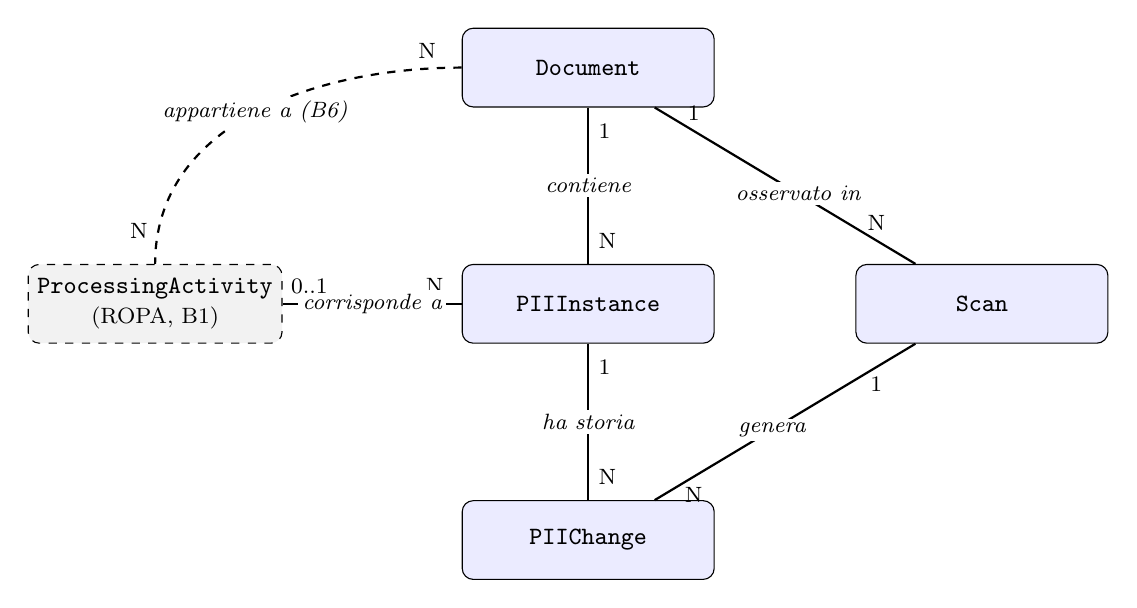
\begin{tikzpicture}[
			entity/.style={rectangle, draw, rounded corners, minimum width=3.2cm,
					minimum height=1cm, align=center, fill=blue!8, font=\small},
			ext/.style={rectangle, draw, dashed, rounded corners, minimum width=3.2cm,
					minimum height=1cm, align=center, fill=gray!10, font=\small},
			rel/.style={font=\footnotesize\itshape, fill=white, inner sep=1.5pt},
			card/.style={font=\footnotesize},
			link/.style={thick},
		]
		\node (doc)  [entity] at (0, 3)    {\texttt{Document}};
		\node (inst) [entity] at (0, 0)    {\texttt{PIIInstance}};
		\node (chg)  [entity] at (0, -3)   {\texttt{PIIChange}};
		\node (scan) [entity] at (5, 0)    {\texttt{Scan}};
		\node (act)  [ext]    at (-5.5, 0) {\texttt{ProcessingActivity}\\{\footnotesize(ROPA, B1)}};

		% Document (1)--(N) PIIInstance : contiene
		\draw [link] (doc) -- node[card, pos=0.15, right]{1}
		node[rel]{contiene} node[card, pos=0.85, right]{N} (inst);
		% PIIInstance (1)--(N) PIIChange : ha storia
		\draw [link] (inst) -- node[card, pos=0.15, right]{1}
		node[rel]{ha storia} node[card, pos=0.85, right]{N} (chg);
		% Document (1)--(N) Scan : osservato in
		\draw [link] (doc) -- node[card, pos=0.15, above]{1}
		node[rel, pos=0.55]{osservato in} node[card, pos=0.85, above]{N} (scan);
		% Scan (1)--(N) PIIChange : genera
		\draw [link] (scan) -- node[card, pos=0.15, below]{1}
		node[rel, pos=0.55]{genera} node[card, pos=0.85, below]{N} (chg);
		% PIIInstance (N)--(0..1) ProcessingActivity : corrisponde a
		\draw [link] (inst) -- node[card, pos=0.15, above]{N}
		node[rel]{corrisponde a} node[card, pos=0.85, above]{0..1} (act);
		% Document (N)--(N) ProcessingActivity : appartiene a (associazione B6, N:N)
		\draw [link, dashed] (doc) to[out=180, in=90]
		node[card, pos=0.08, above]{N}
		node[rel, pos=0.5]{appartiene a (B6)}
		node[card, pos=0.92, left]{N} (act);
	\end{tikzpicture}
	\caption[Diagramma ER del registro delle PII rilevate]{Diagramma entità--relazione del registro delle PII rilevate (blocco B5): lo stato corrente (\texttt{PIIInstance}) e la sua storia (\texttt{PIIChange}), legati alle scansioni (\texttt{Scan}) e ai documenti (\texttt{Document}). I legami con \texttt{ProcessingActivity} del registro ROPA (tratteggiati, blocco B1) sono due: l'associazione \emph{documento--trattamento} (N:N, blocco B6), registrata su \texttt{Document.activity\_ids} con la sua provenienza (\texttt{association\_source}); e il riferimento \emph{per singola PII} (0..1) a un trattamento giustificante, la cui assenza segnala una PII \emph{orfana}, popolato dalla verifica di conformità (B7) a partire dall'associazione stessa. Non mostrata la tabella delle regole cartella→trattamento (\texttt{registry\_folder\_rule}, B6), che alimenta l'associazione per prefisso.}
	\label{fig:er-registro-pii}
\end{figure}

\section{Associazione e verifica di conformità}
\label{sec:conformita}

I blocchi B6 e B7 della Figura~\ref{fig:architettura-macro-blocchi} sono il punto in cui le due metà del sistema --- il \emph{dichiarato} (il ROPA, §\ref{sec:modello-ropa}) e il \emph{rilevato} (il registro delle PII, §\ref{sec:persistenza-registro}) --- si incontrano e producono il \textbf{verdetto di conformità}. Fino a questo punto il sistema sa, separatamente, quali categorie un trattamento \emph{dichiara} e quali PII un documento \emph{contiene}; è il confronto fra i due insiemi a trasformare un rilevatore di PII in uno strumento di \emph{governance}, ed è ciò che distingue il progetto dagli strumenti di sola rilevazione (§\ref{sec:sintesi-gap}).

\subsection{Associazione documento--trattamento (B6)}
\label{sub:b6-associazione}

Il confronto ha senso solo rispetto a un termine di paragone: prima di chiedersi «questo documento è conforme?», bisogna sapere \emph{a quale trattamento} il documento appartiene. È il compito del blocco B6: associare un documento a una o più \texttt{ProcessingActivity} dichiarate.

L'associazione è \textbf{esplicita} --- la stabilisce il DPO, non un'inferenza automatica --- e la scelta è metodologica, non di comodo. Un'associazione \emph{per contenuto}, che attribuisse il documento al trattamento i cui dati dichiarati somigliano di più a quelli rilevati, sarebbe \textbf{circolare}: sceglierebbe per costruzione il trattamento che rende il documento «il più conforme possibile», svuotando di senso la verifica successiva. L'associazione esplicita mantiene invece il confronto \textbf{onesto}: il trattamento è deciso da un umano, e B7 misura poi, senza sconti, ciò che quel trattamento dichiara rispetto a ciò che il documento contiene. L'associazione resta comunque dietro un contratto (\texttt{ActivityAssigner}), così un proponente automatico o assistito dall'AI potrà in futuro \emph{proporre} l'attribuzione lasciando al DPO la conferma --- lo stesso schema \emph{human-in-the-loop} già adottato per la mappatura del ROPA (§\ref{sub:ropa-ai}).

La relazione è \textbf{molti-a-molti}: un documento può rientrare in più trattamenti (un modulo usato tanto nella selezione del personale quanto nelle paghe) e un trattamento raccoglie molti documenti. L'insieme dei trattamenti di un documento è registrato sul documento stesso (\texttt{Document.activity\_ids}); poiché ROPA e registro delle PII vivono su basi dati separate (§\ref{sec:persistenza-registro}), gli identificatori di trattamento fanno da collegamento \emph{logico} fra i due mondi, senza chiave esterna fisica.

Perché l'associazione esplicita sia \textbf{praticabile su cartelle reali} --- dove attribuire un documento alla volta è improponibile --- il DPO dispone di due modalità, entrambe \emph{decise da lui}: l'associazione \textbf{diretta} di un singolo documento e le \textbf{regole cartella→trattamento}, con cui mappa una volta un \emph{prefisso di percorso} a uno o più trattamenti; ogni documento che ricade sotto quel prefisso --- i file nuovi inclusi, alla scansione successiva --- \emph{eredita} l'associazione. Una regola non è un'inferenza per contenuto (che si è appena esclusa perché circolare): resta una scelta esplicita del DPO, solo espressa per \emph{collocazione} anziché documento per documento. La \textbf{provenienza} di ogni associazione è tracciata (\texttt{association\_source}, con valori \texttt{MANUAL} e \texttt{RULE}) e il manuale \textbf{prevale}: riapplicare le regole non sovrascrive mai un'associazione fatta a mano. Le regole si applicano come passo separato \emph{dopo} la scansione, così una scansione schedulata associa da sé i documenti nuovi --- un passo verso l'autonomia «dai una cartella e fa da solo».

\subsection{Il confronto dichiarato--rilevato e il suo vocabolario (B7)}
\label{sub:b7-vocabolario}

Fissata l'associazione, la verifica di conformità è un'operazione \textbf{insiemistica}. Da un lato l'insieme dei \texttt{pii\_type} \emph{dichiarati}: l'unione delle categorie dichiarate da \emph{tutti} i trattamenti a cui il documento è associato. Quali mappature concorrano a formare quell'insieme è un parametro esplicito del confronto: il verdetto \emph{autorevole} considera le sole mappature confermate dal DPO (§\ref{sub:ropa-ai}), mentre la consultazione interattiva conta anche quelle ancora proposte, così da restare informativa prima che la revisione del registro sia stata completata. La distinzione va tenuta presente nel leggere un verdetto, perché la stessa categoria può risultare orfana nell'una lettura e coperta nell'altra; ciò che invece non è ammissibile è che i due criteri convivano \emph{dentro} un medesimo verdetto, e la regola su quali categorie contino è perciò definita in un unico punto e usata da tutti i controlli, conservazione inclusa. Dall'altro l'insieme dei \texttt{pii\_type} \emph{rilevati}: i tipi delle PII effettivamente presenti nel documento secondo il registro. Confrontando i due insiemi, ogni tipo ricade in una voce di un \textbf{vocabolario chiuso}, che è il linguaggio con cui il sistema riporta il verdetto al DPO:

\begin{description}
	\item[Coperta] un tipo \emph{rilevato} che è anche \emph{dichiarato} da almeno uno dei trattamenti associati. È il caso conforme: il dato presente è previsto dal registro.
	\item[Orfana] un tipo \emph{rilevato} che \textbf{nessuno} dei trattamenti associati dichiara. È il segnale di conformità cardine: un dato personale presente nel documento che il ROPA non prevede --- un trattamento di fatto non dichiarato (art.~30 GDPR, art.~12 nLPD). Si dice «orfana» perché priva di un trattamento-genitore che la giustifichi.
	\item[Mancante] un tipo \emph{dichiarato} da un trattamento associato ma \textbf{non} riscontrato nel documento. Non è di per sé una violazione: può indicare una sovra-dichiarazione, oppure semplicemente che quel documento non contiene quel dato.
	\item[Non risolvibile] una categoria \emph{dichiarata} nel ROPA che non si risolve in alcun \texttt{pii\_type} (insieme vuoto, §\ref{sub:ropa-modello}): è dichiarata ma non rilevabile dal motore. Resta esplicita e va segnalata al DPO, invece di essere scambiata per conforme.
\end{description}

Sotto la cardinalità molti-a-molti la definizione di orfana è deliberatamente \textbf{permissiva}: un tipo è orfano solo se \emph{nessuno} dei trattamenti associati lo dichiara (unione, non intersezione). Un dato coperto anche da un solo trattamento pertinente è giustificato. Specularmente, a ogni singola PII rilevata la verifica assegna il primo trattamento associato che ne dichiara il tipo come «trattamento giustificante» (\texttt{processing\_activity\_id}), oppure nessuno se la PII è orfana: è il momento in cui il riferimento opzionale (0..1) lasciato vuoto dal registro (§\ref{sub:persistenza-modello-dati}) viene finalmente popolato.

Due principi ereditati dal resto del sistema governano la lettura del verdetto. Il primo è \textbf{recall-first} (§\ref{sub:b4-merge}): il sistema preferisce segnalare un'orfana di troppo che mancarne una, perché un falso positivo costa al DPO una verifica, mentre una PII non dichiarata e non vista è un rischio invisibile. Il secondo è che il verdetto è un \textbf{segnale, non una sentenza}: un'orfana afferma «non risulta dichiarata», non «è certamente una violazione». Può infatti nascere da una violazione reale oppure da un buco di mappatura a monte --- una categoria del ROPA non ancora risolta sul tipo corrispondente. È il DPO, \emph{human-in-the-loop}, a chiudere il giudizio; il sistema gli mette davanti l'evidenza strutturata.

\subsection{Verifica della conservazione}
\label{sub:b7-retention}

Alla verifica delle categorie si affianca un controllo di \textbf{conservazione} (\textit{retention}): un dato può essere legittimamente dichiarato eppure trattenuto oltre il periodo consentito. Il ROPA porta, a livello di macro-categoria, una durata massima \emph{calcolabile a macchina} (\texttt{retention\_months}, §\ref{sub:ropa-modello}); confrontandola con l'età del documento si segnala una categoria conservata oltre il limite quando un suo dato è ancora presente. La misura dell'età resta una \textbf{stima}, ma dichiarata: la data di riferimento del documento è ricavata dai metadati interni del file quando li possiede (\texttt{modDate} di un PDF, \emph{core properties} dei formati Office) e, in loro assenza, dalla sua ultima modifica sul file system (il \emph{mtime}). Poiché le due fonti non valgono lo stesso --- il \emph{mtime} è azzerato da qualunque copia massiva o ripristino da backup --- il sistema conserva accanto alla data la sua \textbf{provenienza} (§\ref{sec:sv-reference-date}) e la espone nel verdetto, così che una segnalazione fondata su un metadato interno non venga confusa con un indizio da verificare. Sono inoltre distinti due esiti che il primo prototipo confondeva: la \emph{violazione}, quando il documento eccede un termine dichiarato, e la \emph{conservazione non verificabile}, quando il registro esprime un criterio anziché una durata --- caso in cui il silenzio non deve essere scambiato per conformità. Il verdetto è infine consultabile sull'intero corpus, ordinato per mesi di sforamento, e non soltanto documento per documento.

\section{Interfaccia e restituzione al DPO}
\label{sec:report-b8}

Il blocco B8 chiude la catena: rende consultabile ciò che i blocchi precedenti hanno prodotto. La scelta architetturale che lo caratterizza è che il sistema si presenta come una \textbf{applicazione web unica}, servita su una sola porta, e non come una raccolta di comandi da terminale. La ragione è di destinatario: il DPO non è necessariamente una figura tecnica, e uno strumento di conformità utilizzabile solo da chi sa invocare un comando resta, di fatto, inutilizzato. Le interfacce a riga di comando continuano a esistere e sono pienamente funzionali, ma il loro ruolo è quello di strumenti di servizio --- automazione, esecuzioni schedulate, diagnostica --- non di via d'accesso ordinaria.

\paragraph{Una sola applicazione, due interfacce.} La revisione del registro dei trattamenti (B1) e il cruscotto di conformità nascono come applicazioni distinte, con cicli di vita e destinatari in parte diversi; sono però \emph{montate} nella stessa applicazione, che le espone sotto percorsi differenti. Il risultato è un unico servizio da avviare e configurare --- coerente con il requisito di semplicità di installazione (§\ref{sub:facilita-installazione}) --- senza che le due parti debbano fondersi in un solo componente: ciascuna conserva il proprio insieme di pagine e i propri test.

\paragraph{Consultare non deve modificare.} Il cruscotto calcola il verdetto di conformità nel momento in cui una pagina viene aperta, e questo pone un vincolo preciso: la sola consultazione non deve produrre effetti sullo stato del sistema. Il verdetto mostrato in lettura è quindi calcolato in modalità \emph{non persistente}, mentre la scrittura degli esiti per singola PII avviene soltanto in risposta a un'azione esplicita del DPO --- tipicamente l'associazione di un documento a un trattamento. È una distinzione che vale la pena rendere esplicita, perché il medesimo calcolo serve due scopi diversi: informare e registrare.

\paragraph{Riferimenti, mai valori.} La minimizzazione del dato (§\ref{sub:minimizzazione}) non è un vincolo della sola persistenza ma attraversa anche la restituzione: le PII sono presentate al DPO come \emph{riferimenti} --- categoria, posizione nel documento, provenienza del rilevamento, stato di conformità --- e in nessuna schermata compare il valore del dato personale rilevato. Un cruscotto che mostrasse i valori trasformerebbe lo strumento di verifica in una nuova copia dei dati da proteggere, vanificando la scelta compiuta a monte nel registro.

\paragraph{Due letture, per documento e per corpus.} La restituzione è organizzata su due livelli complementari. La vista \emph{per documento} risponde alla domanda «questo file è in regola?» e riunisce in un solo luogo le PII rilevate, l'associazione ai trattamenti e il verdetto. Le viste \emph{per corpus} rispondono invece alle domande che un responsabile pone su un intero archivio --- che cosa è oltre il termine di conservazione, quali documenti nessuna regola ha ancora associato --- e sono ciò che rende lo strumento praticabile su volumi reali, dove l'esame documento per documento non è una procedura eseguibile.

\chapter{Implementazione}
\label{cap:implementazione}

% TODO: INSERIRE QUI "ROADMAP IMPLEMENTATIVA E DI VALIDAZIONE"
% Fare riferimento al file "Training_NER_confronto_strategie.md" (Sezione 5).
% Spiegare i passi dell'implementazione sperimentale:
% 1. Implementazione della baseline con zero-shot GLiNER
% 2. Integrazione e test di un modello pre-fine-tunato (gliner-pii)
% 3. Eventuale esplorazione di fine-tuning solo a scopo esplorativo per il diario tecnico.

% -- B1 --
\section{B1 - Ingestione del ROPA}
\label{sec:impl-b1-ingestione}

Il blocco B1 realizza il percorso che porta un registro dei trattamenti, così come lo compila un'organizzazione, alla rappresentazione interna descritta nel modello di dominio (§\ref{sec:modello-ropa}). La realizzazione segue il principio \emph{sottrattivo} già motivato in architettura --- del documento sorgente si conserva soltanto ciò che alimenta la verifica di conformità --- e lo traduce in una catena di tre passi disaccoppiati (lettura, interpretazione, persistenza), seguìti da una passata separata di mappatura assistita. Ogni passo è un modulo a sé, così che un cambiamento di formato del file o di strategia di mappatura non tocchi gli altri.

\subsection{Il formato sorgente: il template CNIL reale}
\label{sub:impl-b1-formato}

La fonte non è un formato inventato per comodità, ma il \textbf{modello di registro ufficiale della CNIL}, l'autorità francese per la protezione dei dati: un foglio di calcolo (ODS/XLSX) con una scheda operativa (\emph{fiche}) per ciascun trattamento, oltre a schede di servizio (tutorial, elenco dei trattamenti, un modello vuoto da replicare, liste di supporto). Ancorare l'ingestione a un artefatto reale, anziché a un file cucito sul parser, rende la funzionalità dimostrabile su un input che un'organizzazione userebbe davvero. Nella \emph{fiche}, l'ingestione modella \textbf{una sola sezione} --- «\texttt{Categories of personal data}», con le sue colonne \emph{categoria}, \emph{descrizione} e \emph{periodo di conservazione} --- e scarta deliberatamente tutte le altre (attori, finalità secondarie, categorie di interessati, destinatari, trasferimenti, misure di sicurezza), coerentemente con la scelta sottrattiva. È questa sezione, e solo questa, a fornire il dichiarato che B7 confronterà con il rilevato.

\subsection{Lettura: un'unica forma per ODS ed Excel}
\label{sub:impl-b1-lettura}

Il primo passo (\texttt{sheet\_reader}) legge una scheda del foglio in una griglia di stringhe, dietro un'interfaccia \textbf{indipendente dal formato} (\emph{Adapter}): l'estensione del file decide il \textit{back-end} --- \texttt{.ods} tramite \texttt{odfpy}, \texttt{.xlsx}/\texttt{.xlsm} tramite \texttt{openpyxl} --- ma entrambi restituiscono la stessa struttura, così che il passo interpretativo a valle ignori del tutto la provenienza. Un dettaglio pratico del formato ODS ha richiesto attenzione: nel modello CNIL diverse celle portano un \textbf{commento} d'aiuto (il «triangolino rosso»), che nel documento risiede \emph{dentro} la cella come annotazione. Letto ingenuamente, quel testo verrebbe concatenato davanti al valore reale (per esempio «\texttt{Cf.\ Article~87\ldots{}Social Security Number}»); il lettore esclude perciò i paragrafi contenuti nelle annotazioni, restituendo il solo valore della cella. È una piccola scelta di robustezza, ma tocca proprio la sezione che si vuole conservare, e come tale è coperta da test sul file CNIL reale.

\subsection{Interpretazione: guidata dalle etichette, non dalle posizioni}
\label{sub:impl-b1-normalizer}

Il secondo passo (\texttt{normalizer}) trasforma la griglia in un'attività di trattamento. La regola cardine è che le informazioni si cercano per \textbf{etichetta}, non per indice di riga: il nome del trattamento è il valore accanto alla cella «\texttt{Name of the processing operation}», la finalità quello accanto a «\texttt{Main purpose}», e le categorie sono le righe che seguono l'intestazione «\texttt{Categories of personal data}» fino alla prima riga vuota. Così la mappatura \textbf{sopravvive} a spostamenti di righe e alla presenza delle numerose sezioni che non si modellano: il parser vi passa sopra senza inciampare. La stessa regola fa da filtro naturale sulle schede di servizio: una scheda priva del nome di trattamento --- il tutorial, le liste, il modello \emph{vuoto} --- non è un'attività e viene saltata sollevando un errore che il chiamante intercetta, sicché un intero \emph{workbook} CNIL produce esattamente un'attività per ogni \emph{fiche} compilata. Il periodo di conservazione, infine, viene reso \textbf{calcolabile}: la dicitura originale («5 years from the payment of the salary») è conservata per audit accanto a una durata in mesi estratta da essa (60), quando il testo esprime una durata fissa; resta \texttt{None} quando esprime un criterio, coerentemente con il campo del modello (§\ref{sub:dati-ropa}).

\subsection{Persistenza e mappatura assistita}
\label{sub:impl-b1-mappatura}

Tre tabelle rispecchiano la gerarchia a tre livelli del registro CNIL (§\ref{sub:ropa-modello}).

\paragraph{\texttt{processing\_activity} --- l'attività di trattamento (livello 1).}
\begin{description}
	\item[\texttt{id}] identificatore stabile dell'attività (chiave primaria), assegnato dal chiamante; àncora dell'intera sotto-struttura.
	\item[\texttt{name}] nome del trattamento, per leggibilità e report al DPO.
	\item[\texttt{purpose}] finalità dichiarata del trattamento, elemento cardine dell'art.~30 GDPR.
\end{description}

\paragraph{\texttt{macro\_category} --- il blocco di categorie con la sua conservazione (livello 2).}
\begin{description}
	\item[\texttt{id}] chiave surrogata (auto-generata).
	\item[\texttt{activity\_id}] chiave esterna all'attività: colloca la macro-categoria nella gerarchia.
	\item[\texttt{raw\_text}] dicitura originale della macro-categoria, conservata \emph{tale e quale} per auditabilità (nulla del documento sorgente va perduto).
	\item[\texttt{retention\_text}] dicitura originale del periodo di conservazione, conservata per audit.
	\item[\texttt{retention\_months}] la stessa conservazione resa \textbf{calcolabile dalla macchina} (durata in mesi), affinché il controllo di retention (B7) sia un confronto e non una lettura di prosa; vale \texttt{None} quando il registro esprime un criterio anziché una durata fissa.
\end{description}

\paragraph{\texttt{declared\_category} --- la categoria dichiarata, ponte verso il rilevamento (livello 3).}
\begin{description}
	\item[\texttt{id}] chiave surrogata.
	\item[\texttt{macro\_category\_id}] chiave esterna alla macro-categoria di appartenenza.
	\item[\texttt{raw\_text}] testo libero originale della categoria (es.\ «nome»), conservato per audit.
	\item[\texttt{pii\_types}] l'insieme di \texttt{pii\_type} del catalogo condiviso a cui la categoria è ricondotta: è l'\textbf{aggancio} che rende il confronto fra ciò che il ROPA \emph{dichiara} e ciò che il motore \emph{rileva} (B7) una semplice operazione insiemistica.
	\item[\texttt{mapping\_state}] stato del mapping (\texttt{PROPOSED} dall'AI / \texttt{CONFIRMED} dal DPO): materializza il \emph{human-in-the-loop}: l'AI propone la corrispondenza, ma non la fissa mai da sola.
\end{description}

Il terzo passo affida l'attività così ottenuta al \texttt{ROPARepository}, che la scrive nella base dati ROPA riusando lo stesso modello di dominio come schema (\emph{Active Record}, §\ref{sec:dati-persistiti}). La \textbf{risoluzione delle categorie sui \texttt{pii\_type}} del catalogo condiviso --- l'aggancio verso il rilevamento --- è invece una passata \textbf{separata e successiva}, non parte del parsing deterministico: per ogni categoria ancora non risolta, una strategia dietro il contratto \texttt{CategoryMapper} propone i \texttt{pii\_type} corrispondenti al suo testo libero. La strategia è intercambiabile --- un \textbf{dizionario} deterministico (parole chiave), un \textbf{modello generativo} (§\ref{sec:scelta-modello-llm}) o una combinazione dei due --- e la passata è \textbf{idempotente}: ciò che il mapper non sa risolvere resta invariato, così una riesecuzione mappa solo ciò che è nuovo. Il risultato è comunque una \emph{proposta}: lo stato del mapping resta \texttt{PROPOSED} finché il DPO non lo conferma (\emph{human-in-the-loop}, §\ref{sub:ropa-ai}), a ribadire che l'AI arricchisce ma non decide.

L'interazione del DPO avviene tramite un'interfaccia web dedicata (blocco B8, la review montata sotto \texttt{/ropa}), da cui può confermare le mappature, \textbf{importare} un nuovo registro caricandone il file dal browser --- il file viaggia verso il servizio come \emph{byte} via \emph{multipart}, coerente con il deployment containerizzato in cui l'applicazione non accede al file system del client --- e \textbf{rimuovere} un trattamento. L'import riusa senza modifiche la catena di ingestione appena descritta: la stessa lettura, la stessa interpretazione, la stessa mappatura.

% ============================================================================
% SCAFFOLDING (temporaneo) — mappa parallela §6 (idea) <-> §7 (realizzazione).
% Speculare a quello in 6_architettura.tex. Struttura dati DENTRO i blocchi.
% In §7 buona parte c'e' gia' (persistenza, container): riempire i buchi B3/B4/
% B6/B7/B8. Eliminare a lavoro finito.
% ----------------------------------------------------------------------------
% B2 - Analisi struttura FS: nulla in §7 (non implementato).  |  §6: perche' non fatto.
% ----------------------------------------------------------------------------
% B3 - Estrazione del testo
%   §7 (come): lettori PDF/DOCX/txt + fogli + .doc legacy; extraction/dates.py
%       (metadati->mtime, guardia <1990/futuro, degrado grazioso).
%   §6 (idea): born-digital -> testo normalizzato + reference_date con provenienza.
% ----------------------------------------------------------------------------
% B4 - Detection (espandere §"Realizzazione del livello di rilevamento", gia' presente)
%   §7 (come): Presidio pattern+NER + GLiNER; RegexDetector config-driven (fatto);
%       + MergeEngine; + LLMDetector (prompt catalogo chiuso, valore->span via
%       str.find, chunking, never-raise); + slot opzionale ai + AITriggerPolicy
%       (hash stabile); benchmark run_ai_benchmark (P/R/F1, s/doc, Wh/doc).
%   §6 (idea): due sorgenti dietro PIIDetector + merge (4 casi) + ramo generativo.
% ----------------------------------------------------------------------------
% B5 - Registro PII: GIA' in §"Dati persistiti" (document/scan/instance).
%   NB: changelog per-PII (NEW/CONFIRMED/MOVED/REMOVED, tabella change) SCARTATO,
%   rimosso da §7 (vedi rimozione-tempo.md). NON re-introdurlo in §6.
%   Da aggiungere: freshness (scansione incrementale) e refresh CONFIRMED.
%   §6 (idea): due orologi (impronta file vs data semantica), minimizzazione.
% ----------------------------------------------------------------------------
% B6 - Associazione + regole cartella
%   §7 (come): FolderRule (tabella gia' in "Dati persistiti"); riconciliazione
%       (azzera RULE stale); auto-apply a fine scan.
%   §6 (idea): esplicita + prefisso->attivita' + provenienza + ponte cross-DB.
% ----------------------------------------------------------------------------
% B7 - Conformita' + conservazione
%   §7 (come): checker.build_report; vista di corpus /retention; propose_category
%       (orfana -> DeclaredCategory PROPOSED, solo su conferma DPO).
%   §6 (idea): should/is -> orfane/coperte/mancanti; retention + non-verificabile;
%       dalla orfana alla proposta (il feedback).
% ----------------------------------------------------------------------------
% B8 - Dashboard DPO
%   §7 (come): app FastAPI unica (una porta); pagine (dashboard / documento /
%       /retention / /scan / /rules; review ROPA montata sotto /ropa); trigger AI
%       (menu campionamento, per-documento ASINCRONO via ScanJob); due fasi;
%       indicatore di scansione attiva.
%   §6 (idea): restituzione al DPO; human-in-the-loop; Post/Redirect/Get.
% ----------------------------------------------------------------------------
% TRASVERSALE: §7 "Deployment containerizzato" (FATTO).  §6: sezione "Pattern
%   di progettazione" (nuova). Principi una volta sola: recall-first, minimizzazione, DPO sovrano.
% ============================================================================

% -- B3 --
\section{B2 - Analisi struttura file system}
\label{sec:impl-b2-analisi-fs}
Non realizzato, motivazioni nella sezione al capitolo precedente (\ref{sec:b2-analisi-struttura}) e in sviluppi futuri (\ref{cap:sviluppi-futuri}).

% -- B3 --
\section{B3 - Estrazione del testo}
\label{sec:impl-b3-estrazione}

L'estrazione è realizzata da \texttt{extract\_document(path)}, che dall'estensione del file sceglie il lettore appropriato e restituisce un \texttt{NormalizedDocument} (il testo più l'identità del documento). I reader sono volutamente leggeri --- uno per famiglia di formato, con \emph{import} lazy, così che l'assenza di una dipendenza non pesi su chi non la usa --- e coprono i formati più diffusi in ambito \emph{consumer} ed \emph{enterprise}~\cite{sonacollegeoftechnologyindiaFRAMEWORKANALYSINGUNSTRUCTURED2021}:
\begin{itemize}
	\item \texttt{.pdf} tramite PyMuPDF (testo \emph{born-digital});
	\item \texttt{.docx} tramite python-docx;
	\item \texttt{.txt} per lettura diretta;
	\item i fogli \texttt{.xlsx}/\texttt{.xlsm}/\texttt{.ods} riusando il \texttt{sheet\_reader} del blocco B1 (openpyxl/odfpy), con le celle rese come testo;
	\item il Word \emph{legacy} \texttt{.doc} tramite il binario di sistema \texttt{antiword}, presente nell'immagine container (assente in locale, il file finisce in errore e il lotto prosegue).
\end{itemize}
L'elenco dei formati ha un'unica fonte (\texttt{supported\_suffixes()}), così che anteprima, scansione e lettore lo ereditino senza divergere. OCR, layout multi-colonna e formati come \texttt{.xls}/\texttt{.rtf} restano fuori ambito (§\ref{cap:sviluppi-futuri}).

Accanto al testo, l'estrazione stima la \textbf{data di riferimento} del documento (\texttt{extraction/dates.py}), che alimenta il controllo di conservazione (B7, §\ref{sub:b7-retention}). \texttt{reference\_date(path)} interroga per primi i metadati interni del file --- \texttt{modDate}/\texttt{creationDate} del PDF, le \emph{core properties} di DOCX e XLSX --- e ricade sul \emph{mtime} del file system solo quando non trova nulla di utilizzabile, restituendo un \texttt{ReferenceDate} che porta con sé la \textbf{provenienza} (\texttt{DateSource}: \texttt{content\_metadata} oppure \texttt{file\_mtime}), sicché il verdetto di conformità può dichiarare quanto vale la stima che espone. Un'unica guardia di plausibilità scarta le date anteriori al 1990 o collocate nel futuro e passa al candidato successivo; metadati illeggibili non sollevano un'eccezione ma ricadono sul \emph{mtime} --- datare un documento non deve poter interrompere la sua analisi.

% -- TECNOLOGIA DI PERSISTENZA (da capire se tenere così o scorporare) --
\section{Tecnologia di persistenza}
\label{sec:implementazione-persistenza-tecnologia}

Il modello concettuale della persistenza --- il registro delle PII rilevate (§\ref{sec:persistenza-registro}) e la gerarchia del registro ROPA (§\ref{sec:modello-ropa}) --- è \textit{technology-agnostic}: restava da fissare la tecnologia concreta con cui realizzarlo. I candidati erano due:
\begin{itemize}
	\item una base dati \textbf{relazionale} (SQLite), che offre \textit{join} e interrogazioni relazionali «gratuite» ed è coerente col deployment locale in container senza servizi esterni;
	\item una persistenza \textbf{su file semi-strutturati} (JSON/JSONL), più leggera ma priva di garanzie relazionali native.
\end{itemize}

La scelta è ricaduta su \textbf{SQLite}, per ragioni che discendono dalla natura del dato e dai vincoli di progetto:
\begin{itemize}
	\item \textbf{Il dato è intrinsecamente relazionale.} Entrambi i registri sono grafi di entità legate da chiavi esterne (documento--scansione--istanza; attività--macro-categoria--categoria) e le interrogazioni che servono ai blocchi a valle --- stato corrente di un documento, PII orfane, confronto dichiarato-vs-rilevato --- sono \textit{join} e operazioni insiemistiche che un motore relazionale risolve nativamente. Su file JSON andrebbero reimplementate a mano, riscrivendo ciò che un DBMS offre già.
	\item \textbf{SQLite è \emph{embedded}, senza server.} È un singolo file, nessun processo o servizio esterno da gestire: coerente col deployment containerizzato e, soprattutto, con la \textbf{minimizzazione del dato} --- i dati non lasciano l'infrastruttura on-premise e nessun servizio di terzi è coinvolto.
	\item \textbf{Una sola definizione (\textit{Active Record}).} Con SQLModel l'entità di dominio \emph{è} la tabella (§\ref{sec:dati-persistiti}): niente coppia dominio/riga né traduzione a mano, coerente col principio DRY.
	\item \textbf{La porta resta aperta.} SQLModel poggia su SQLAlchemy: migrare a un RDBMS in rete (ad esempio PostgreSQL), qualora si superi il singolo nodo, cambia l'URL di connessione --- letto da variabile d'ambiente (§\ref{sec:containerizzazione}) --- e non il modello dei dati. SQLite è dunque la scelta adeguata \emph{ora}, non un vicolo cieco.
\end{itemize}

La stessa tecnologia serve entrambi i registri, su due basi dati separate (variabili d'ambiente \texttt{ROPA\_DB\_URL} e \texttt{PII\_DB\_URL}); \emph{che cosa} vi si conserva, campo per campo, è dettagliato nel §\ref{sec:dati-persistiti}.

\section{Dati persistiti nei database}
\label{sec:dati-persistiti}

Il sistema mantiene due basi dati distinte e separate (§\ref{sec:containerizzazione}): il \textbf{registro ROPA} (blocco B1) e il \textbf{registro delle PII rilevate} (blocco B5). Ogni entità è definita una sola volta come tabella SQLModel --- il modello di dominio \emph{è} lo schema di persistenza (\textit{Active Record}) --- così da non duplicare la struttura. I modelli concettuali e le relazioni sono discussi in §\ref{sub:ropa-modello} e §\ref{sub:persistenza-modello-dati}; questa sezione documenta, \textbf{campo per campo, ciò che viene effettivamente scritto su disco e perché}. La realizzazione corrente è su SQLite (§\ref{sec:implementazione-persistenza-tecnologia}), ma il modello dei dati qui descritto è indipendente dalla tecnologia sottostante.

Un principio attraversa entrambe le basi ed è la chiave di lettura di ogni campo che segue: la \textbf{minimizzazione del dato} (§2.3.11). In particolare il registro delle PII conserva soltanto \emph{riferimenti} --- tipo, posizione, provenienza, documento --- e \textbf{mai il valore} della PII, come si vedrà nell'assenza deliberata di una colonna che lo contenga.

% -- B4 --
\section{B4 - Livello di rilevamento}
\label{sec:impl-detection}

Le due scelte tecnologiche che governano questo livello --- costruire il rilevamento a pattern e NER sopra Microsoft Presidio, e quale modello generativo adottare per gli impieghi selettivi --- non sono state compiute qui: sono l'esito degli studi condotti prima della progettazione (§\ref{sec:valutazione-presidio}, §\ref{sec:scelta-modello-llm}), la cui verifica sperimentale è nel Capitolo~\ref{cap:test}. Questa sezione ne descrive la realizzazione, e in particolare la proprietà che ne governa la manutenzione nel tempo.

\subsection{Estensibilità config-driven: aggiungere categorie e pattern}
\label{sub:estensibilita-detection}

Una proprietà di progetto del livello di rilevamento è che il suo vocabolario non è cablato nel codice ma \textbf{dichiarato in configurazione}. Il catalogo delle categorie di PII (\texttt{categories.yaml}) e i pattern a espressioni regolari personalizzati (\texttt{custom\_patterns.yaml}) sono file validati al caricamento; aggiungere una nuova categoria o un nuovo identificatore strutturato --- un codice aziendale, un riferimento interno, un numero di settore --- è quindi una \textbf{modifica di configurazione, non di codice}. Le regole così dichiarate vengono eseguite a runtime dal riconoscitore generico (\texttt{RegexDetector}) e affiancate ai riconoscitori pre-costruiti di Presidio tramite un \texttt{CompositeDetector}, così da presentarsi al merge come un'unica sorgente di pattern.

La scelta separa \emph{ciò che} si rileva --- competenza del DPO o del manutentore, in configurazione --- da \emph{come} lo si rileva, cioè il motore, che resta stabile. Il file dei pattern personalizzati è riservato agli identificatori che Presidio non copre nativamente (il numero AVS svizzero ne è il primo esempio), per non duplicare ciò che il motore già fornisce. La validazione al caricamento --- il pattern deve compilare, ogni \texttt{pii\_type} deve esistere nel catalogo --- fa fallire subito una configurazione errata, invece di degradare il rilevamento in silenzio. Resta fuori, come sviluppo dichiarato, la validazione a \emph{checksum} degli identificatori: un pattern è riconosciuto per forma, non verificato nel contenuto.

\subsection{Presidio come engine}
\label{sub:impl-presidio}

Il rilevamento a pattern e a NER poggia su un unico motore, l'\texttt{AnalyzerEngine} di Microsoft Presidio~\cite{HomeMicrosoftPresidio}, che è la dipendenza portante del livello: il sistema non riscrive i riconoscitori, li orchestra. Presidio è usato come \textbf{black box} --- riceve il testo e restituisce i riscontri (tipo di entità, intervallo di caratteri, punteggio), senza che il sistema ne governi gli interni --- con una precisazione che conta: non gli si dice \emph{quali} PII cercare; il motore riporta tutte le entità che i suoi riconoscitori conoscono, ed è il sistema a \textbf{filtrarle e ricondurle} al proprio catalogo.

L'incrocio fra le entità di Presidio e il vocabolario dei \texttt{pii\_type} del sistema è \textbf{dichiarato in configurazione} (\texttt{presidio\_entities.yaml}): un'entità mappata diventa un candidato del tipo corrispondente, un'entità non mappata viene scartata. Quando la NER è affidata a GLiNER~\cite{zaratianaGLiNERGeneralistModel2023} (§\ref{sec:scelta-modello-llm}) si aggiunge un secondo passaggio dichiarativo --- dalle etichette \emph{zero-shot} di GLiNER alle entità di Presidio --- così che la rotta verso il catalogo resti una sola.

Una sottigliezza realizzativa merita di essere detta, perché è ciò che tiene \emph{indipendenti} le due sorgenti che il merge poi confronta (§\ref{sub:b4-merge}). Presidio mescola in un solo engine i riconoscitori a pattern e quelli a NER; da quello \emph{stesso} analizzatore il sistema costruisce \textbf{due} detector distinti --- uno trattiene i soli riscontri a pattern, l'altro quelli a NER, separati per il nome del riconoscitore che li ha prodotti. Senza questa separazione le due tecniche sarebbero un'unica sorgente e non potrebbero \emph{concordare}: non esisterebbe la doppia conferma. Gli identificatori che Presidio non copre nativamente --- il numero AVS svizzero --- sono infine aggiunti dal \texttt{RegexDetector} guidato da configurazione e composti coi riconoscitori di Presidio in un'unica sorgente di pattern (\texttt{CompositeDetector}, §\ref{sub:estensibilita-detection}).

\subsection{Il detector generativo}
\label{sub:impl-ai-detector}

Il terzo rilevatore --- il ramo generativo (§\ref{sub:b4-ai-previsto}) --- è realizzato dietro lo stesso contratto \texttt{PIIDetector} degli altri (\texttt{LLMDetector}), così da entrare nel merge e nella misura senza codice speciale. Al modello locale si chiedono i \emph{valori} delle PII, non i loro offset --- che un modello linguistico non sa contare in modo affidabile --- e ciascun valore è poi \textbf{rilocalizzato} cercandone le occorrenze nel testo: un valore inventato che nel documento non compare non viene trovato, ed è la prima difesa contro le allucinazioni; la seconda è il catalogo chiuso nel prompt, contro cui ogni tipo proposto è validato.

Il modello è scelto da una variabile d'ambiente dedicata, \texttt{PII\_LLM\_MODEL}, \textbf{distinta} da quella del mapper del ROPA (\texttt{ROPA\_LLM\_MODEL}): le due funzionalità AI possono così adottare pesi diversi, pur puntando per default allo \emph{stesso} modello già presente nell'immagine container --- \texttt{phi4-mini}~\cite{abouelenin2025phi4mini} --- scelto per leggerezza e per non introdurre dipendenze. Di questa scelta va detto anche il limite: un modello piccolo e a inferenza rapida non è l'ideale per \emph{leggere} documenti di molte pagine, dove un modello più capace renderebbe di più. La virtù dell'impostazione è che sostituirlo costa una sola variabile d'ambiente --- il \emph{runtime} (Ollama) serve il nuovo modello senza altri interventi --- ed è per questo che la scelta del peso è demandata alla misura (§\ref{cap:risultati}) anziché cablata. \emph{Quali} documenti ricevano il secondo parere è deciso, fuori dal rilevatore, dalla politica di campionamento descritta in architettura (§\ref{sub:b4-ai-previsto}); i riscontri, comunque prodotti, portano con sé la provenienza generativa che il registro conserva (§\ref{sub:dati-registro-pii}), ed è quella provenienza --- \emph{quale} detector ha trovato \emph{che cosa} --- ad abilitare i gradi di certezza del merge.

% -- B5 --
\subsection{Registro delle PII rilevate (blocco B5)}
\label{sub:dati-registro-pii}

% BOZZA B5 (§7) — resa fisica del registro-snapshot descritto in §\ref{sec:b5-DB-PII}. Rivedere.
Queste tabelle sono la \textbf{resa fisica} del registro-snapshot descritto in architettura (§\ref{sec:b5-DB-PII}): conservano lo stato corrente delle PII per documento --- non la loro storia nel tempo, semplificazione motivata fra gli sviluppi futuri (§\ref{sec:sf-tracciamento-temporale}) --- e mai il valore del dato (minimizzazione, §\ref{sub:minimizzazione}), come si vede campo per campo qui sotto.

Tre tabelle realizzano il registro delle PII rilevate (§\ref{sub:persistenza-modello-dati}): il documento, la scansione e la singola istanza rilevata, che ne è lo \textbf{stato corrente}. Una quarta tabella, \texttt{registry\_folder\_rule}, risiede nella stessa base dati ma appartiene al blocco di associazione (B6, §\ref{sub:b6-associazione}) ed è descritta in coda a questa sezione. È nella tabella delle istanze che la minimizzazione si vede nel dettaglio.

\paragraph{\texttt{registry\_document} --- il documento analizzato.}
\begin{description}
	\item[\texttt{document\_id}] identificatore stabile del documento (chiave primaria), coerente con il \texttt{document\_id} prodotto da B3; nella scansione ricorsiva di una cartella è il \textbf{percorso relativo} (POSIX) alla radice, ciò che consente alle regole cartella→trattamento di combaciare per prefisso (§\ref{sub:b6-associazione}).
	\item[\texttt{path}] percorso originale del file, come riferimento; opzionale.
	\item[\texttt{first\_seen}] istante di prima registrazione del documento.
	\item[\texttt{activity\_ids}] gli identificatori dei trattamenti dichiarati a cui il documento è associato (B6): è una \textbf{lista} (cardinalità N:N, §\ref{sub:b6-associazione}) e i suoi valori riferiscono \texttt{ProcessingActivity} nell'altra base dati, come collegamento \emph{logico} senza chiave esterna fisica.
	\item[\texttt{association\_source}] la \textbf{provenienza} dell'associazione --- \texttt{MANUAL} (impostata dal DPO) oppure \texttt{RULE} (derivata da una regola cartella→trattamento) --- oppure \texttt{None} se il documento non è ancora associato. È il campo che fa \textbf{vincere il manuale sulle regole}: riapplicare le regole salta i documenti a provenienza \texttt{MANUAL}.
	\item[\texttt{reference\_date}] la data cui il documento si assume risalga, letta dai metadati interni del file quando li possiede e dal file system altrimenti, usata come età del contenuto per il controllo \emph{approssimato} di conservazione (B7, §\ref{sub:b7-retention}); è un \emph{riferimento}, non un valore di PII. Vale \texttt{None} se ignota.
	\item[\texttt{reference\_date\_source}] la provenienza della data precedente (\texttt{content\_metadata} o \texttt{file\_mtime}), perché il verdetto possa dichiarare quanto vale la stima che espone.
	\item[\texttt{source\_mtime}, \texttt{source\_size}] l'impronta \emph{tecnica} del file osservata all'ultima analisi --- da non confondere con la data semantica: serve unicamente a stabilire se il file sia cambiato e vada quindi rianalizzato (§\ref{sec:sv-due-orologi}).
	\item[\texttt{last\_scanned\_at}] il momento dell'ultima analisi effettiva del documento; una scansione in cui esso venga omesso perché invariato non lo aggiorna.
	\item[\texttt{detector\_signature}] l'impronta della configurazione di rilevamento con cui le istanze correnti sono state prodotte: se cambia, il documento va rianalizzato anche a file immutato.
\end{description}
Il vocabolario di \texttt{association\_source} è un'enumerazione chiusa (\texttt{AssociationSource}: \texttt{MANUAL}/\texttt{RULE}), come per gli altri campi a dominio fissato del modello.

\paragraph{\texttt{registry\_scan} --- una singola esecuzione di analisi.}
\begin{description}
	\item[\texttt{id}] chiave surrogata.
	\item[\texttt{document\_id}] chiave esterna al documento analizzato.
	\item[\texttt{created\_at}] istante in cui la scansione è stata eseguita.
\end{description}

\paragraph{\texttt{registry\_pii\_instance} --- la singola PII, stato corrente e mutabile.}
Nessuna colonna di questa tabella contiene il \emph{valore} della PII: è il punto in cui la minimizzazione diventa concreta.
\begin{description}
	\item[\texttt{id}] chiave surrogata.
	\item[\texttt{document\_id}] chiave esterna al documento che la contiene.
	\item[\texttt{pii\_type}] la categoria del catalogo condiviso (es.\ \texttt{iban}) --- \emph{non} il valore.
	\item[\texttt{start}, \texttt{end}] la \textbf{posizione} come intervallo di caratteri nel testo normalizzato: un riferimento a \emph{dove} si trova la PII, non al suo contenuto.
	\item[\texttt{confidence}] confidenza aggregata dal merge, per consentire al DPO ordinamento e soglie.
	\item[\texttt{confirmation\_level}] esito del merge (\texttt{single\_source} / \texttt{double\_confirmed} / \texttt{conflicting} / \texttt{ai\_discovered}): traccia \emph{quanto} è certa la rilevazione.
	\item[\texttt{sources}] gli identificatori dei detector che l'hanno trovata: traccia \emph{chi} l'ha rilevata (tracciabilità, §2.7.3).
	\item[\texttt{processing\_activity\_id}] l'attività dichiarata a cui la PII corrisponde, oppure \texttt{None} se la PII è \textbf{orfana} (non riconducibile ad alcun trattamento); popolata dal blocco di associazione (B6), senza chiave esterna fisica finché i due database restano distinti.
	\item[\texttt{last\_scan\_id}] chiave esterna alla scansione che ha registrato l'istanza.
\end{description}
Ogni scansione \textbf{sostituisce} le istanze del documento con ciò che vi trova ora: la tabella descrive lo \textbf{stato corrente} delle PII del documento, non la loro storia nel tempo.
L'\textbf{assenza} di un campo \texttt{value}/\texttt{text} è una scelta di progetto, non una dimenticanza: garantisce che un registro di conformità non si trasformi a sua volta in un archivio di dati personali.

% ---- RIMOSSO: tracciabilità temporale per-PII (changelog delta-based) scartata --------
% Feature a metà, troppo complessa: non fatta perenne. Vedi rimozione-tempo.md.
% RIMOSSA ANCHE DAL CODICE (2026-08-20): via ChangeType/PIIChange/diff.py, record_scan
% ora replace-on-scan. La tabella registry_pii_change NON esiste più. Blocco tenuto
% commentato solo come traccia storica; si può eliminare del tutto.
% \paragraph{\texttt{registry\_pii\_change} --- il log append-only delle variazioni.}
% \begin{description}
% 	\item[\texttt{id}] chiave surrogata.
% 	\item[\texttt{pii\_instance\_id}] chiave esterna all'istanza cui la variazione si riferisce.
% 	\item[\texttt{change\_type}] il tipo di variazione, vocabolario chiuso: \texttt{NEW} / \texttt{CONFIRMED} / \texttt{MOVED} / \texttt{REMOVED}.
% 	\item[\texttt{scan\_id}] chiave esterna alla scansione che ha prodotto la variazione.
% 	\item[\texttt{previous\_scan\_id}] chiave esterna alla scansione \emph{precedente} dello stesso documento --- ciò che lega le rilevazioni nel tempo; vale \texttt{None} alla prima scansione (\emph{bootstrap}).
% 	\item[\texttt{timestamp}] istante in cui la variazione è stata registrata.
% \end{description}
% ---- fine blocco rimosso ---------------------------------------------------------------

\paragraph{\texttt{registry\_folder\_rule} --- la regola cartella→trattamento (blocco B6).}
Fisicamente nella stessa base dati del registro delle PII, ma logicamente parte dell'associazione (§\ref{sub:b6-associazione}): mappa un prefisso di percorso ai trattamenti che i documenti sotto di esso ereditano.
\begin{description}
	\item[\texttt{prefix}] il prefisso di percorso (POSIX, normalizzato senza slash finale; \texttt{""} è la radice e combacia con ogni documento). Chiave primaria.
	\item[\texttt{activity\_ids}] i trattamenti con cui associare i documenti che cadono sotto \texttt{prefix}; riferiscono \texttt{ProcessingActivity} nell'altra base dati (nessuna chiave esterna fisica), come \texttt{Document.activity\_ids}.
	\item[\texttt{created\_at}] istante di creazione della regola.
\end{description}

In sintesi: il registro ROPA conserva il dichiarato (con il testo originale accanto alla forma strutturata, per audit), mentre il registro delle PII conserva soltanto \emph{riferimenti} a ciò che è stato rilevato --- mai i valori. Le due basi restano separate; i campi \texttt{Document.activity\_ids} (associazione N:N, B6) e \texttt{PIIInstance.processing\_activity\_id} (trattamento giustificante per singola PII, popolato da B7) sono i punti in cui i due mondi si collegano \emph{logicamente}, sull'identificatore-stringa del trattamento.

% -- B7 --
\section{B7 - Verifica di conformità}
\label{sec:impl-b7-conformita}

% NB: qui va la realizzazione di B7. Per ora è scritto il solo controllo di
% conservazione (splittato dal §6, §\ref{sub:b7-retention}); il confronto
% dichiarato-vs-rilevato (checker.build_report -> orfane/coperte/mancanti,
% propose_category) resta da riempire.

\subsection{Il controllo di conservazione}
\label{sub:impl-b7-retention}

Il concetto del controllo di conservazione è in architettura (§\ref{sub:b7-retention}); qui se ne descrive la realizzazione. Il verdetto confronta la durata dichiarata dal ROPA --- \texttt{retention\_months} della macro-categoria (§\ref{sub:dati-ropa}) --- con l'\textbf{età del documento}, cioè la sua \texttt{reference\_date} con la relativa provenienza (\texttt{DateSource}), stimata dall'estrazione (§\ref{sec:impl-b3-estrazione}): una categoria è in \emph{violazione} quando un suo dato è ancora presente e la data del documento supera il termine dichiarato.

Il caso più insidioso non è la violazione ma il \textbf{silenzio}. Quando la macro-categoria non esprime una durata fissa ma un criterio (\texttt{retention\_months} vale \texttt{None}, per esempio «per la durata del rapporto»), il primo prototipo saltava il controllo e il documento usciva \emph{conforme} senza che nessuno avesse verificato. Ora quel caso produce l'esito esplicito \texttt{retention\_unresolved} (\emph{conservazione non verificabile}), calcolato \textbf{fuori} dalla guardia sulla data --- la lacuna è nel registro, non nel documento --- così da distinguerlo dalla conformità effettiva. La \textbf{regola su quali categorie contino} (solo le confermate, oppure anche le proposte) è definita in un unico punto (\texttt{\_macro\_types}) e usata identica dal confronto delle categorie e dal controllo di conservazione, perché uno stesso documento non possa risultare orfano per metà verdetto e coperto per l'altra.

Due dettagli di robustezza completano il quadro. Il parsing del periodo di conservazione riconosce anche le \textbf{unità francesi} (\texttt{an}/\texttt{ans}/\texttt{mois}): il template è quello CNIL e una dicitura come «5 ans» non riconosciuta disattiverebbe di fatto il controllo. E la stessa lettura è disponibile come \textbf{vista di corpus} (\texttt{compliance retention} da CLI, pagina \texttt{/retention} nella dashboard): riusa lo stesso calcolo su tutto il registro, legge il ROPA \textbf{una sola volta}, non scrive nulla e ordina i documenti per mesi di sforamento; i documenti non associati ad alcun trattamento sono esclusi, perché senza un termine dichiarato non c'è nulla da confrontare.

\section{Deployment containerizzato e portabilità}
\label{sec:containerizzazione}

La containerizzazione non è un dettaglio di confezionamento, ma un \textbf{requisito di progetto} --- l'installazione deve avvenire tramite un meccanismo standardizzato e riproducibile --- e un corollario diretto dell'architettura: i componenti sono concepiti come \textbf{servizi raggiungibili su porta e configurati da variabili d'ambiente}, con l'applicazione nel ruolo di interfaccia leggera. È inoltre funzionale alla \textbf{minimizzazione del dato}: tutti i servizi risiedono nella rete privata dell'orchestrazione e i dati trattati non lasciano l'infrastruttura on-premise. Questa sezione fissa l'approccio di deployment adottato e ne descrive la realizzazione.

\subsection{Portabilità e isolamento delle dipendenze}
\label{sub:container-portabilita}

L'obiettivo operativo è una build \textbf{riproducibile su qualsiasi piattaforma}: la stessa immagine deve girare identica in sviluppo e in produzione, indipendentemente dall'architettura dell'host. L'argomento più forte a favore emerge da un problema concreto incontrato nello sviluppo. Il livello di rilevamento NER poggia su uno \textit{stack} di apprendimento automatico pesante e fragile (PyTorch e il modello NER GLiNER); sulla macchina di sviluppo --- un interprete Python \texttt{x86\_64} in emulazione su hardware ARM --- la versione di PyTorch disponibile risultava troppo datata per la restante toolchain (NumPy, transformers), rendendo il livello NER \textbf{non costruibile in locale}. Un container Linux, con dipendenze moderne, risolve il problema alla radice e --- punto generale --- \textbf{disaccoppia la build dall'architettura dell'host}: ciò che in locale è un vicolo cieco diventa, nel container, l'ambiente di riferimento in cui la stessa immagine è riproducibile ovunque. La containerizzazione non è quindi soltanto un requisito formale, ma la risposta pragmatica alla fragilità delle dipendenze di apprendimento automatico.

\subsection{Architettura di deployment}
\label{sub:container-architettura}

Il sistema è orchestrato come un insieme di servizi. Il \textbf{servizio applicativo} racchiude il nucleo --- ingestione ROPA, motore di detection con i livelli regex/checksum e NER, verifica di conformità, interfaccia per il DPO --- insieme alle relative dipendenze, comprese quelle di apprendimento automatico più onerose (Presidio, spaCy, GLiNER), che nell'immagine Linux si installano senza attriti. Il \textbf{runtime del modello generativo} --- un servizio \textbf{Ollama} (basato su \texttt{llama.cpp}) che serve lo SLM scelto (§\ref{sec:scelta-modello-llm}) su porta, con host e nome del modello letti da variabili d'ambiente (\texttt{OLLAMA\_HOST}, \texttt{ROPA\_LLM\_MODEL}) --- è un container separato, coerente con l'uso selettivo e non ricorrente dell'AI. La \textbf{base dati} è, allo stato attuale, un file SQLite su volume persistente (§\ref{sec:implementazione-persistenza-tecnologia}). Tutta la configurazione --- URL della base dati, host e nome del modello --- è letta da \textbf{variabili d'ambiente}, così la stessa immagine gira in locale e in container cambiando solo la configurazione; i pesi dei modelli e lo stato della base dati vivono su \textbf{volumi} dedicati, per non essere riscaricati o persi tra un'esecuzione e l'altra. Coerentemente col profilo hardware del progetto (§\ref{sec:valutazione-presidio}), tutti i servizi operano su \textbf{CPU}.

\subsection{Contratti e direzione}
\label{sub:container-direzione}

Il disaccoppiamento è garantito dai contratti già introdotti all'interno dell'architettura: \texttt{PIIDetector} per i rilevatori, \texttt{CategoryMapper} per la normalizzazione del ROPA, un client astratto per il modello generativo. Poiché ogni funzionalità dipende solo dalla \textit{forma} del contratto e non dalla sua collocazione, \textbf{spostare una funzionalità in un sotto-container dedicato ha un costo quasi nullo}. La direzione è quindi l'articolazione progressiva in \textbf{sotto-container per funzionalità}: il runtime generativo è già un servizio a sé; il livello NER, oggi in-process, è scorporabile in un servizio dedicato qualora se ne debba scalare il carico; la persistenza migrerà da SQLite a una base dati relazionale in rete (ad esempio PostgreSQL) quando si superi il singolo nodo. Rimane come sviluppo la pubblicazione di immagini \textbf{multi-architettura} (amd64/arm64). Il container costituisce la via canonica per eseguire il sistema completo, dipendenze di apprendimento automatico incluse, mentre il nucleo leggero resta eseguibile nativamente per l'iterazione rapida di sviluppo.
\chapter{Test e validazione}
\label{cap:test}

\section{Validazione del livello di rilevamento}
\label{sec:test-detection}

\textbf{DA AGGIORNARE}

Le scelte lasciate aperte in fase di implementazione --- se costruire il livello regex/NER sopra Microsoft Presidio (§\ref{sec:valutazione-presidio}) e quale motore di NER adottare --- sono qui chiuse su base empirica.

\paragraph{Metodo.} La valutazione riusa l'impianto di scoring del progetto: un corpus annotato di documenti sintetici in cui ogni PII è marcata con il proprio \texttt{pii\_type} e la sua posizione. Un rilevamento conta come vero positivo quando condivide il \texttt{pii\_type} con uno span di \textit{ground truth} e vi si sovrappone con \textit{Intersection over Union} $\geq 0.5$; ogni rilevamento e ogni span sono appaiati al più una volta (\textit{matching} greedy). Da qui si derivano precision, recall e F1 micro-mediati. Ogni configurazione è incapsulata dietro il contratto \texttt{PIIDetector} e misurata sullo stesso corpus, così da confrontarle sullo stesso metro.

\paragraph{Risultati.} Il confronto è nella Tabella~\ref{tab:test-detection}. \textbf{Il livello a pattern di Presidio} (espressioni regolari e checksum) supera la baseline regex proprietaria (F1 0.85 contro 0.79) con precisione perfetta e senza falsi positivi, e copre nativamente categorie che la baseline mancava; viene quindi adottato, coerentemente con la scelta di incapsularlo dietro \texttt{PIIDetector} (§\ref{sec:valutazione-presidio}). Per il \textbf{livello NER}, il modello generico spaCy si rivela inadeguato: F1 0.08, con recall quasi nullo e falsi positivi (etichetta come \textit{location} identificatori strutturati, ad esempio un IBAN). Sostituendolo con \textbf{GLiNER}, NER \textit{zero-shot} specifico per le PII, il livello NER sale a F1 0.44 e --- dato decisivo --- la detection completa (pattern + NER) passa da F1 0.77 a \textbf{0.89}: GLiNER chiude i buchi del NER, portando \texttt{address} da 0 a F1 1.00 e il recall di \texttt{person\_name} a 1.00.

\begin{table}[htbp]
	\centering
	\caption{Validazione del livello di rilevamento sul corpus annotato (P, R, F1).}
	\label{tab:test-detection}
	\small
	\begin{tabular}{|l|c|c|c|}
		\hline
		\textbf{Configurazione}                  & \textbf{P}    & \textbf{R}    & \textbf{F1}   \\
		\hline
		Baseline regex (proprietaria)            & 0.93          & 0.68          & 0.79          \\
		\hline
		Presidio --- solo pattern/checksum       & 1.00          & 0.74          & 0.85          \\
		\hline
		NER spaCy (\texttt{it\_core\_news\_lg})  & 0.17          & 0.05          & 0.08          \\
		\hline
		NER GLiNER (\texttt{gliner\_multi\_pii}) & 0.75          & 0.32          & 0.44          \\
		\hline
		Presidio (pattern + NER spaCy)           & 0.75          & 0.79          & 0.77          \\
		\hline
		\textbf{Presidio (pattern + NER GLiNER)} & \textbf{0.89} & \textbf{0.89} & \textbf{0.89} \\
		\hline
	\end{tabular}
\end{table}

\paragraph{Limiti.} Il corpus è ridotto (poche decine di span) e sintetico: i valori vanno letti come \textbf{direzionali}, non come stime definitive, e la loro conferma richiede un corpus più ampio e realistico. Restano inoltre due punti aperti: la precisione di GLiNER su \texttt{person\_name} è ancora migliorabile (over-tagging occasionale), e l'inferenza GLiNER su CPU è più lenta di spaCy --- accettabile, trattandosi di un modello \textit{encoder} e non generativo, ma da tenere presente per il livello di rilevamento ricorrente (blocco B4).

\chapter{Risultati e discussione}
\label{cap:risultati}

Questo capitolo raccoglie le considerazioni maturate nei vari capitoli di questo lavoro e rilegge le misure del Capitolo~\ref{cap:test} alla luce delle domande poste all'inizio, traendone due conclusioni. La prima riguarda ciò che è stato costruito: un sistema funzionante e misurato, che risponde a un bisogno concreto e potrebbe essere impiegato così com'è. La seconda, che costituisce il baricentro della tesi, riguarda l'AI generativa: un lavoro nato come esplorazione del suo apporto al rilevamento delle PII ne ridimensiona il ruolo sulla base dei dati raccolti durante le sperimentazioni.

% =====================================================================
\section{Il sistema realizzato}
\label{sec:risultati-sistema}
% =====================================================================

Al netto della questione generativa, il lavoro ha prodotto un \textbf{prototipo funzionante e misurato} che copre l'intera catena dal documento all'esito di conformità. A partire da una cartella di documenti non strutturati, il sistema ne estrae il testo (§\ref{sec:impl-b3-estrazione}), vi rileva le categorie di dati personali fondendo pattern e NER (§\ref{sec:impl-detection}), registra le PII trovate come \emph{riferimenti} minimizzati --- tipo, posizione, provenienza, mai il valore (§\ref{sub:dati-registro-pii}) ---, associa i documenti alle attività dichiarate nel registro dei trattamenti (§\ref{sec:b6-documento-trattamento}) e restituisce un esito di conformità leggibile dal DPO: categorie orfane, coperte, mancanti e superamento dei termini di conservazione (§\ref{sec:impl-b7-conformita}). È esattamente l'insieme degli obiettivi enunciati all'inizio (§\ref{sec:obiettivi}), realizzato end-to-end e operabile da un'interfaccia web unica (§\ref{sec:b8-dashboard}).

Sul metro sperimentale, la parte di rilevamento coglie quasi tutto ciò che deve trovare. La pipeline tradizionale raggiunge una \textbf{recall di 0.99} sul corpus aziendale, misurata sull'insieme completo dei $300$ documenti e delle $2918$ occorrenze annotate (Tabella~\ref{tab:test-pattern}, Tabella~\ref{tab:test-ner}). Il degrado misurato fra testo pulito e testo estratto dai file reali è nullo (Tabella~\ref{tab:test-estrazione}), sicché su documenti \emph{born-digital} lo stadio di estrazione si può considerare trasparente. La precisione è invece più bassa ($0.66$ sul campione su cui è tabulata la pipeline fusa, Tabella~\ref{tab:test-detection-confronto}), con una causa circoscritta a una sola categoria: il riconoscimento dei \emph{nomi di persona}, dove l'\textit{encoder} NER etichetta come tali molte espressioni che non lo sono, raccoglie da solo circa due terzi di tutti i falsi positivi, proporzione che si conferma sia sul campione sia sull'intero corpus. Il difetto è reale ma di natura benigna per l'uso previsto, poiché produce lavoro di revisione per il DPO anziché rischi di conformità non visti, ed è coerente con l'impostazione \textit{recall-oriented} del \emph{merge} (§\ref{sub:b4-merge}), che preferisce deliberatamente un falso positivo a una PII mancata. Trattandosi di numeri ottenuti su corpus sintetici, essi vanno letti come \emph{limite superiore} (§\ref{sub:test-estrazione}) più che come garanzia sul campo; bastano però a stabilire che l'impianto scelto --- Presidio con GLiNER, fusi da un motore di \textit{merge} \textit{recall-oriented} --- è adeguato al compito per cui è stato adottato, e a indicare con precisione dove andrebbe migliorato.

Oltre all'accuratezza, il sistema risponde a un \textbf{bisogno normativo concreto e mal coperto dal mercato}. L'obbligo di sapere dove stanno i dati personali, a quale trattamento si riferiscono e se sono ancora entro i termini di conservazione discende direttamente dalla nLPD (art.~6(4)) e dal GDPR (art.~5(1)(e), art.~30), mentre nella pratica gran parte di quei dati vive dispersa in documenti non strutturati, fuori da ogni visibilità sistematica (§\ref{sec:progetto-assegnato}). Gli strumenti commerciali esistenti sono tarati su GDPR o CCPA e non trattano nativamente le categorie della nLPD svizzera, e solo i prodotti \textit{enterprise} più avanzati integrano il registro dei trattamenti come riferimento dichiarativo. Il differenziale del sistema qui realizzato consiste proprio in quel collegamento: le PII rilevate sono \emph{confrontate con il dichiarato} e ne deriva un esito di conformità, che è il valore aggiunto per il DPO.

Il sistema è inoltre \textbf{impiegabile già oggi}, senza prerequisiti onerosi. Gira su hardware \textit{commodity} in un \textit{container} portabile (§\ref{sec:containerizzazione}), non richiede né GPU né addestramento su dati dell'organizzazione (§\ref{sec:considerazioni-training}), è coerente con la minimizzazione del dato per requisito --- i valori delle PII non vengono mai persistiti (§\ref{sub:dati-registro-pii}) --- e rileva a un costo contenuto in tempo ed energia (${\sim}11.8$~s e ${\sim}0.066$~Wh a documento, Tabella~\ref{tab:test-ai-benchmark}), il che lo rende eseguibile con continuità sull'intero patrimonio documentale. Restano naturalmente i limiti dichiarati --- assenza di OCR e di analisi di \textit{layout}, un solo profilo utente, corpus di valutazione sintetici (Capitolo~\ref{cap:sviluppi-futuri}) --- nessuno dei quali ostacola un impiego reale nello scenario per cui il sistema è stato pensato: documenti nativi digitali di un'organizzazione soggetta alla normativa sulla privacy.

% =====================================================================
\section{Costo e apporto dell'AI generativa}
\label{sec:risultati-ai}
% =====================================================================

Il secondo risultato riguarda l'apporto dell'AI generativa, e ne ridimensiona il ruolo rispetto a un'aspettativa largamente condivisa. Il modello generativo è oggi presentato, ben oltre l'ambito tecnico, come soluzione pressoché universale ai problemi di trattamento del testo, da preferire per principio agli approcci tradizionali. Applicata al rilevamento sistematico delle PII, tale aspettativa non trova riscontro nei dati raccolti: sul compito qui studiato l'impiego generativo comporta un costo superiore di un ordine di grandezza, in tempo e in energia, senza un corrispondente guadagno di qualità.

La conclusione arriva da due direzioni convergenti. Da un lato la letteratura la anticipa in termini generali (§\ref{sec:impatto-ambientale}): a parità di compito, un modello discriminativo consuma circa 0.002~kWh ogni 1000 inferenze contro le ${\sim}0.047$~kWh di un generativo, e sul piano economico il divario fra un \textit{encoder} e un modello generativo di frontiera arriva a rapporti dell'ordine di 300:1. Dall'altro --- ed è il contributo proprio di questo lavoro --- la misura diretta sul sistema reale conferma il divario e ne fissa l'entità sul \emph{nostro} hardware e sul \emph{nostro} compito. Il rilevamento tradizionale opera a ${\sim}11.8$~s e ${\sim}0.066$~Wh per documento; ogni passata generativa costa fra $40$ e $83$~s e fra $0.41$ e $0.76$~Wh per documento (Tabella~\ref{tab:test-ai-benchmark}): da ${\sim}3$ a ${\sim}7\times$ più lenta, da ${\sim}6$ a ${\sim}12\times$ più energivora. Va osservato che il divario, misurato su documenti reali, risulta inferiore a quello che la letteratura riporta su singole inferenze: entrambi i termini crescono con la lunghezza del testo, e su documenti estesi anche il rilevamento tradizionale sostiene il costo dell'\textit{encoder} NER sull'intero contenuto.

A tale costo non corrisponde un guadagno di qualità \emph{per il sistema}. La pipeline tradizionale raggiunge F1 $0.79$ sul corpus aziendale, e l'aggiunta del parere generativo la lascia invariata: le configurazioni di fusione --- le uniche operative, poiché il rilevatore generativo affianca i rilevatori tradizionali anziché sostituirli --- si collocano fra $0.76$ e $0.79$, ossia al più eguagliano la baseline (Tabella~\ref{tab:test-detection-confronto}). Il meccanismo è quello atteso: la fusione recupera occorrenze e porta la recall a $1.00$, introducendo però falsi positivi che riportano la precisione a $0.61$ e ne riassorbono il vantaggio.

Preso isolatamente, il rilevatore generativo restituisce un quadro meno netto, che va riportato con esattezza. Dei due modelli misurati uno ottiene una F1 superiore a quella della baseline, l'altro le resta sensibilmente al di sotto: da due osservazioni discordi si ricava che l'esito \textbf{dipende dal modello}, non una proprietà generale dell'approccio generativo, mentre il costo resta superiore di un ordine di grandezza per entrambi. Va inoltre osservato il modo in cui il primo ottiene il proprio vantaggio: la sua recall è $0.85$ contro lo $0.99$ della baseline, ossia rileva \emph{meno} PII, e la F1 gli risulta favorevole soltanto perché quell'indicatore pesa allo stesso modo precisione e recall. La pesatura non corrisponde alle priorità del dominio: una PII non rilevata è un rischio di conformità che resta invisibile, mentre un falso positivo si traduce in lavoro di revisione per il DPO. Il sistema riconosce tale asimmetria adottando un \emph{merge} a impostazione \textit{recall-oriented} (§\ref{sub:b4-merge}); sulla dimensione che per questo compito conta di più il rilevatore generativo resta perciò indietro.

Neppure la taglia del modello incide favorevolmente, e in questo caso il vincolo si manifesta prima ancora della qualità: il modello da 12B della stessa famiglia \textbf{non è risultato eseguibile} nel bersaglio di \textit{deployment} dichiarato. La memoria che esso occupa e quella dell'\textit{encoder} NER eccedono insieme quanto una macchina \textit{commodity} da 16\,GB può garantire, e tre configurazioni successive hanno perso fra il 27\% e il 40\% delle finestre di testo per interruzione del processo di inferenza (§\ref{sec:test-ai-multimodello}). La fascia superiore è perciò esclusa dal confronto quantitativo, con una precisazione che ne delimita la portata: non si afferma che un modello da 12B produrrebbe risultati peggiori, bensì che nel perimetro che il progetto si è dato --- esecuzione locale su hardware ordinario, imposta dalla minimizzazione del dato e non da una preferenza --- quel modello non è disponibile. Analoga esclusione vale per il modello \textit{reasoning}, che presenta la combinazione meno favorevole fra costo e risultato (§\ref{sec:test-ai-multimodello}).

È stata infine verificata l'ipotesi che a penalizzare l'AI sia la sola esecuzione su CPU, e il controllo l'ha esclusa: su GPU la medesima inferenza è ${\sim}9\times$ più veloce e di qualità identica (§\ref{sub:test-gpu}), poiché l'accelerazione riguarda la velocità del calcolo e lascia intatta la sua accuratezza. Quell'accelerazione non è d'altronde disponibile nel bersaglio di \textit{deployment} containerizzato, dove la GPU non è esposta alla macchina virtuale.

La \textbf{portata} di questa conclusione va delimitata con precisione. Non si tratta di un rifiuto dell'AI generativa in quanto tale, bensì della constatazione che, \emph{su questo compito e su questo tipo di dato}, il suo costo non risulta compensato. Il compito è il rilevamento \emph{sistematico e ricorrente} --- ogni documento, ripetutamente --- ed è la ricorrenza a moltiplicare il costo unitario fino a renderlo decisivo (§\ref{sec:impatto-ambientale}). La grandezza determinante è il \textbf{tempo} più che la spesa in valore assoluto, che resta di pochi centesimi: a decine di secondi per documento, una scansione che per via tradizionale richiede minuti si estende a giorni. Il dato in esame è inoltre regolare e nativo digitale, ossia il regime più favorevole ai rilevatori tradizionali, nel quale pattern e NER sono già prossimi al massimo delle loro prestazioni e lasciano all'AI un margine di scoperta minimo. Le condizioni nelle quali il parere generativo potrebbe invece risultare vantaggioso --- testo rumoroso o proveniente da OCR, formati inusuali, PII non strutturate che né i pattern né il NER prevedono --- sono esattamente quelle che i corpus impiegati non riproducono, e restano una questione aperta (§\ref{sec:sf-direzioni}). La scelta architetturale adottata è coerente con questa lettura: l'AI è mantenuta e collocata dove il suo costo non si moltiplica per il corpus --- uno slot \textbf{opzionale e campionato} nel rilevamento (§\ref{sec:impl-detection}) e i pochi compiti \emph{selettivi} a bassa frequenza (§\ref{sec:scelta-modello-llm}) --- riservandola ai casi in cui le interrogazioni sono poche e la comprensione semantica apporta un valore che gli altri approcci non possono dare.

La lezione metodologica va oltre il singolo sistema. Di fronte a un problema di trattamento del testo la domanda pertinente non è se l'AI generativa lo risolva, poiché quasi sempre la risposta è affermativa, ma se lo risolva \emph{meglio} degli approcci più semplici, in misura sufficiente a giustificarne il costo alla scala e alla frequenza d'uso previste. Per il rilevamento sistematico delle PII, misure alla mano, la risposta è negativa: la via tradizionale è sufficientemente accurata, più veloce di un ordine di grandezza e sostenibile con continuità.

% =====================================================================
\section{Considerazioni conclusive}
\label{sec:risultati-chiusura}
% =====================================================================

I due risultati si intersecano. Il sistema realizzato dimostra che la conformità alla nLPD sul contenuto documentale reale è affrontabile immediatamente, con mezzi leggeri e riproducibili; lo studio sull'AI generativa spiega \emph{perché} quei mezzi sono leggeri: la leggerezza è un esito misurato e non una rinuncia, poiché la via più costosa non avrebbe reso di più. Il contributo di questo lavoro consiste dunque in un prototipo funzionante e, insieme, in una risposta quantitativa e documentata a una domanda che spesso si dà per scontata: sul rilevamento sistematico dei dati personali l'approccio tradizionale è la scelta migliore.

Entrambi i risultati poggiano su un artefatto che il lettore può esaminare: il codice del sistema, i generatori dei corpus e la procedura che produce le misure discusse in questi due capitoli sono pubblicati in un repository ad accesso aperto \cite{algisi2026piidiscovery}, alla versione consegnata insieme a questa tesi. La scelta è coerente con il criterio che il Capitolo~\ref{cap:stato-arte} ha usato per giudicare gli strumenti esistenti (§\ref{sub:quadro-comparativo}): un lavoro che rimprovera alle suite commerciali di non essere ispezionabili deve, per primo, esporre il proprio funzionamento alla verifica.

\chapter{Sviluppi futuri}
\label{cap:sviluppi-futuri}

Nel corso del lavoro sono state concepite alcune funzionalità che non sono state realizzate.
Non si tratta di omissioni né di lavoro rimasto incompiuto per mancanza di tempo: sono
\textbf{decisioni}, prese confrontando ciò che ciascuna avrebbe aggiunto con ciò che sarebbe
costata, e va reso conto tanto delle une quanto delle altre. Un progetto che documenta solo
ciò che ha costruito racconta metà del proprio percorso, e non consente a chi lo riprende di
capire se una strada sia stata esclusa perché senza sbocco o semplicemente non tentata. \medskip

Il criterio applicato non è stato «questa funzionalità è utile?», domanda a cui tutte e tre
rispondono affermativamente, bensì il concorso di tre condizioni: il \textbf{valore} che la
funzionalità porta all'utilizzatore, il \textbf{costo} della sua realizzazione, e il
\textbf{contributo metodologico}, ossia se essa produca un risultato misurabile e discutibile
in sede di tesi oppure sia lavoro di realizzazione che nulla aggiunge alla domanda di
ricerca. È soprattutto la terza condizione a spiegare gli esiti che seguono: a parità di
utilità pratica, una funzionalità che non genera alcun dato da valutare compete con il
tempo destinato a ciò che invece ne genera. \medskip

Le sezioni che seguono trattano una funzionalità ciascuna secondo lo stesso schema --- che
cosa avrebbe portato, che cosa sarebbe costata, perché è stata accantonata e a quali
condizioni potrebbe essere ripresa --- e la Tabella~\ref{tab:funzionalita-scartate} ne
riassume la valutazione. L'ultima sezione raccoglie invece i limiti già dichiarati altrove
nel documento, che restano aperti come naturale prosecuzione del lavoro svolto.

\section{Analisi contestuale della struttura del file system}
\label{sec:sf-analisi-struttura}
L'idea, formulata fra i requisiti funzionali (cfr.~\ref{sub:analisi-filesystem}) e prevista
in architettura come blocco autonomo (cfr.~\ref{sec:b2-non-realizzato}), era di trattare
l'\textbf{organizzazione delle cartelle} come un segnale: i nomi dei rami, la profondità e
il raggruppamento dei documenti dicono qualcosa sulla finalità per cui quei documenti sono
tenuti insieme. Nella forma più economica immaginata, l'ingresso sarebbe stato la resa
testuale dell'albero prodotta da un comune comando di sistema --- poche decine di righe di
testo per un'intera condivisione --- da sottoporre a un modello linguistico. \medskip

Il valore atteso era duplice: \textbf{proporre} automaticamente l'associazione fra rami
dell'albero e attività di trattamento, che oggi il DPO stabilisce a mano, e segnalare le
\emph{anomalie posizionali}, ossia i documenti il cui contenuto non è coerente con la
cartella che li ospita. È un valore reale, e resta l'unico modo per far emergere una
violazione del principio di limitazione della finalità che non sia già visibile nel
confronto fra dati rilevati e dati dichiarati. \medskip

Il costo, però, non sta dove sembra. Procurarsi l'ingresso è banale; interpretarlo non lo è.
Un'inferenza sul significato di una struttura di cartelle è un'euristica, e un'euristica va
\textbf{misurata}: servirebbe un corpus di alberi documentali annotati con l'attribuzione
«corretta» di ciascun ramo, che non esiste e andrebbe costruito sinteticamente, raddoppiando
di fatto l'apparato di valutazione (cfr.~\ref{sub:rischio-dataset}) per una funzionalità
accessoria. A ciò si aggiunge un problema di merito: un'attribuzione inferita dalla macchina
diventa il presupposto del verdetto di conformità, che verrebbe così a poggiare su una
supposizione anziché su una dichiarazione. \medskip

La ragione decisiva dell'accantonamento è tuttavia un'altra: la parte \emph{utile} della
funzionalità è stata ottenuta per altra via. Le regole che associano un prefisso di percorso
a una o più attività (cfr.~\ref{sub:b6-associazione}) producono lo stesso effetto operativo
--- associare un intero ramo in un solo gesto, inclusi i documenti che vi compariranno in
seguito --- con la differenza sostanziale che a stabilire il significato della collocazione è
il DPO. Ciò che resterebbe da realizzare non è quindi l'associazione, ma la sola
\emph{proposta} di quelle regole: un incremento reale ma marginale, che presuppone comunque
l'apparato di valutazione appena descritto. La funzionalità è perciò rinviata, e la sua forma
naturale di ripresa è quella di un proponente che suggerisca regole al DPO senza mai
applicarle da sé.

\section{Canale di segnalazione dai dipendenti}
\label{sec:sf-feedback-loop}
Il secondo requisito rimasto sulla carta (cfr.~\ref{sub:feedback-loop}) prevedeva un canale
attraverso cui il personale dell'organizzazione potesse segnalare al DPO i dati personali
incontrati nel lavoro quotidiano, sfuggiti al rilevamento automatico. Il DPO avrebbe
valutato le segnalazioni e le avrebbe usate per arricchire il registro dei trattamenti o i
parametri di rilevamento, secondo il ciclo illustrato nella
Figura~\ref{fig:human-in-the-loop}.
\begin{figure}[htbp]
	\centering
	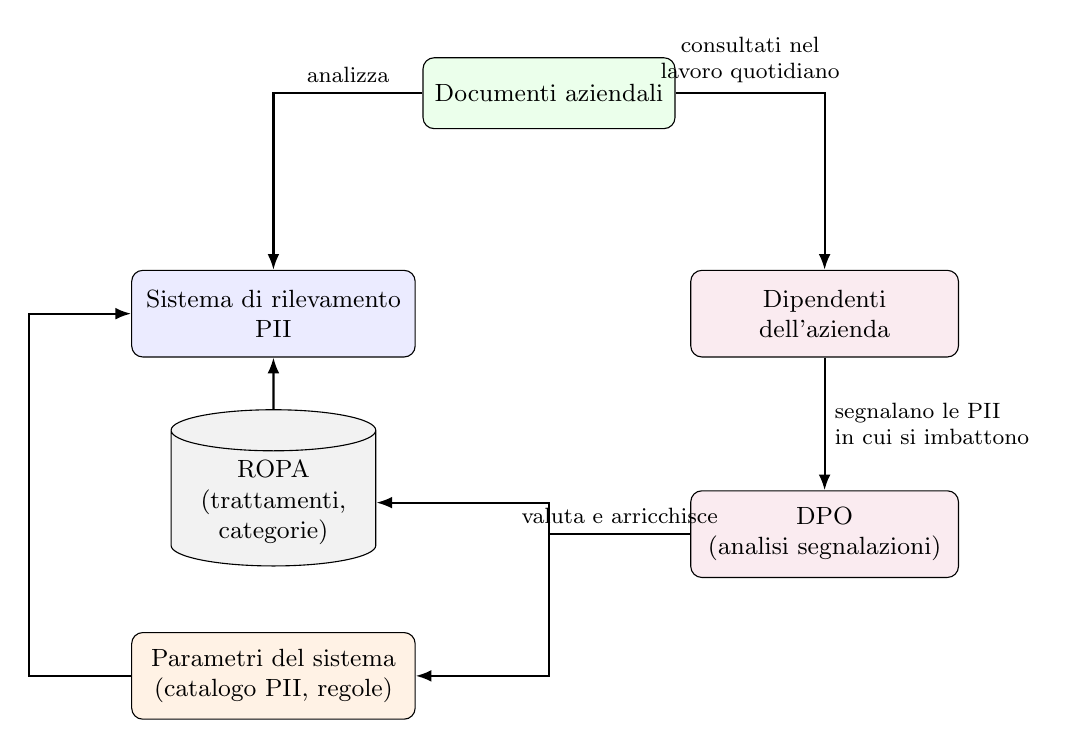
\begin{tikzpicture}[
			sysnode/.style={rectangle, draw, rounded corners, minimum width=3.6cm,
					minimum height=1.1cm, align=center, fill=blue!8, font=\small},
			human/.style={rectangle, draw, rounded corners, minimum width=3.4cm,
					minimum height=1.1cm, align=center, fill=purple!8, font=\small},
			store/.style={cylinder, draw, shape border rotate=90, aspect=0.25,
					minimum height=1.5cm, minimum width=2.6cm, align=center, fill=gray!10, font=\small},
			param/.style={rectangle, draw, rounded corners, minimum width=3.6cm,
					minimum height=1.1cm, align=center, fill=orange!10, font=\small},
			io/.style={rectangle, draw, rounded corners, minimum width=3.2cm,
					minimum height=0.9cm, align=center, fill=green!8, font=\small},
			arrow/.style={thick, -{Latex[length=2mm]}},
		]

		% --- Nodi ---
		% I documenti sono l'artefatto condiviso: analizzati dal sistema e, in
		% parallelo, consultati dai dipendenti nel loro lavoro ordinario. I
		% dipendenti restano ignari del rilevamento: per loro sono solo documenti.
		\node (docs)  [io]      at (3,    1.4)  {Documenti aziendali};
		\node (sys)   [sysnode] at (-0.5, -1.4) {Sistema di rilevamento\\PII};
		\node (emp)   [human]   at (6.5,  -1.4) {Dipendenti\\dell'azienda};
		\node (dpo)   [human]   at (6.5,  -4.2) {DPO\\(analisi segnalazioni)};
		\node (ropa)  [store]   at (-0.5, -3.8) {ROPA\\(trattamenti,\\categorie)};
		\node (param) [param]   at (-0.5, -6.0) {Parametri del sistema\\(catalogo PII, regole)};

		% --- I documenti: analizzati dal sistema, consultati dai dipendenti ---
		\draw [arrow] (docs) -| node[pos=0.25, above, font=\footnotesize]{analizza} (sys.north);
		\draw [arrow] (docs) -| node[pos=0.25, above, font=\footnotesize, align=center]{consultati nel\\lavoro quotidiano} (emp.north);

		% --- Segnalazione: dipendenti -> DPO ---
		\draw [arrow] (emp) -- node[right, font=\footnotesize, align=left]{segnalano le PII\\in cui si imbattono} (dpo);

		% --- Fork: il DPO valuta e arricchisce ROPA e parametri ---
		\coordinate (fk) at (3, -4.2);
		\draw [thick] (dpo.west) -- node[above, font=\footnotesize]{valuta e arricchisce} (fk);
		\draw [arrow] (fk) |- (ropa.east);
		\draw [arrow] (fk) |- (param.east);

		% --- Gli aggiornamenti rientrano nel sistema, che analizza meglio i documenti ---
		\draw [arrow] (ropa) -- (sys);
		\draw [arrow] (param.west) -- ++(-1.3,0) |- (sys.west);

	\end{tikzpicture}
	\caption{Meccanismo di \emph{human-in-the-loop}: nel normale lavoro con i
		documenti aziendali i dipendenti segnalano al DPO le PII in cui si imbattono;
		il DPO analizza le segnalazioni e arricchisce il ROPA o i parametri del
		sistema, migliorando il rilevamento. Il processo di analisi resta trasparente
		ai dipendenti, per i quali i file sono semplici documenti.}
	\label{fig:human-in-the-loop}
\end{figure}
Il valore atteso era il più alto dei tre, e mirava al punto più debole del sistema. I falsi
negativi sono per definizione invisibili (cfr.~\ref{sub:rischio-falsi-negativi}): nessuna
misura interna può rivelare un dato personale che il rilevatore non vede. I dipendenti sono
l'unico sensore che osserva i documenti nel loro contesto d'uso, e sono quindi l'unica
sorgente capace di chiudere quella cecità dall'esterno. \medskip

Il costo è però sproporzionato, e per una ragione strutturale più che di quantità di lavoro.
Il sistema è progettato per un \textbf{unico profilo di utilizzatore}, il DPO, e su questa
premessa poggia l'intera restituzione: una sola interfaccia, che espone senza distinzioni
tutto ciò che il sistema sa. Occorre qui evitare un equivoco: proteggere quella console con
un'autenticazione è cosa dovuta e di costo trascurabile, ed è annoverata fra gli interventi
da compiere (cfr.~\ref{sec:sf-direzioni}); ciò che è oneroso non è \emph{autenticare}, ma
\textbf{autorizzare}. Aprire un canale al personale significherebbe passare da un'identità a
un insieme di identità da censire e mantenere allineato all'organico, e con esso introdurre
ruoli, permessi differenziati, un'interfaccia distinta per chi non deve vedere la console, la
notifica e la moderazione delle segnalazioni. È questa la parte preponderante del lavoro,
mentre la funzionalità in sé si riduce a un modulo di inserimento. \medskip

Vi è inoltre un argomento che da solo sconsiglia la realizzazione nella forma prevista. Il
registro delle rilevazioni non contiene i valori dei dati personali, ma ne costituisce la
\textbf{mappa}: dice dove si trovano, ed è per questo un artefatto sensibile
(cfr.~\ref{sub:rischio-sicurezza-dati}). Esporre a tutto il personale un'interfaccia
affacciata su quel registro significherebbe ampliarne la superficie di accesso dalla singola
figura del DPO all'intera organizzazione: un peggioramento del livello di sicurezza in uno
strumento che esiste per ridurre l'esposizione dei dati. \medskip

A questo si aggiunge la considerazione che ha determinato l'esito: la funzionalità è un
\textbf{processo organizzativo}, non una tecnica di rilevamento. Non produce alcun risultato
misurabile --- non migliora una metrica, non consente un confronto, non sostiene né confuta
un'ipotesi --- e il suo effetto dipende interamente dalla partecipazione delle persone, che
un prototipo non può mettere alla prova. È lavoro di realizzazione che non alimenta la
domanda di ricerca. La funzionalità è pertanto esclusa dal perimetro, e non semplicemente
rinviata; qualora venisse ripresa, la forma corretta sarebbe un canale di sola immissione,
separato dalla console del DPO e privo di qualsiasi accesso in lettura al registro.

\section{Estensione dei formati documentali}
\label{sec:sf-formati}
Il requisito di estrazione (cfr.~\ref{sub:estrazione-testo}) è soddisfatto sui formati
\textit{born-digital} dell'ufficio --- documenti impaginati, videoscrittura, fogli di calcolo
e testo semplice. Restano fuori i documenti che sono immagini, ossia le scansioni, e con essi
il riconoscimento ottico dei caratteri, i layout complessi a più colonne e le tabelle, oltre
ai formati meno diffusi. Allo stato attuale se ne fa a meno: i lettori impiegati sono
sufficienti ai formati coperti, e nessun motore di analisi documentale più elaborato è stato
introdotto. Qualora l'insieme dei formati da trattare venisse ampliato, sarebbe questo il
punto in cui valutare l'adozione di uno strumento dedicato --- Docling o analoghi --- in
luogo dei lettori specifici per singolo formato. \medskip

Il valore è reale ma \textbf{lineare}: ogni formato aggiunto rende leggibile un'altra fetta
del patrimonio documentale, e nulla più. Non cambia ciò che il sistema sa fare, ma solo su
quanti documenti riesce a farlo --- il che, va detto, in un archivio reale con anni di
scansioni può non essere poco. \medskip

Anche il costo è in larga parte lineare, ed è per questo che la funzionalità è stata giudicata
senza contributo di ricerca: lavoro meccanico, ripetitivo e senza decisioni
interessanti da prendere. Il riconoscimento ottico fa però eccezione, perché introduce un
salto qualitativo: non è un lettore in più, è una \textbf{nuova sorgente di errore} collocata
a monte del rilevamento. Il testo che ne esce contiene errori di trascrizione, e ogni PII non
rilevata diventerebbe attribuibile indifferentemente al rilevatore o all'estrattore. \medskip

È quest'ultimo il motivo per cui l'estensione non è stata affrontata ora: la valutazione
misura deliberatamente la \emph{tassa di estrazione} come grandezza distinta dalle prestazioni
del rilevamento (cfr.~Capitolo~\ref{cap:test}), e introdurre un estrattore rumoroso avrebbe
confuso le due sorgenti di errore proprio mentre le si stava separando. La funzionalità resta
rinviata ed è, delle tre, quella ripresa con il minor rischio: il perimetro è contenuto, il
contratto di estrazione già in essere non cambia, e l'ordine ragionevole è affrontare prima i
formati testuali residui e solo dopo, isolandone la misura, il riconoscimento ottico.

\section{Quadro riassuntivo}
\label{sec:sf-quadro}

\begin{table}[htbp]
	\centering
	\caption{Valutazione delle funzionalità concepite e non realizzate.}
	\label{tab:funzionalita-scartate}
	\small
	\resizebox{\textwidth}{!}{%
		\begin{tabular}{|l|c|c|l|c|}
			\hline
			\textbf{Funzionalità}                        & \textbf{Valore} & \textbf{Costo} & \textbf{Contributo metodologico}     & \textbf{Esito}   \\
			\hline
			Analisi della struttura del file system (B2) & Medio           & Alto           & Basso: la parte utile è già ottenuta & Rinviata         \\
			\hline
			Segnalazione dai dipendenti                  & Alto            & Alto           & Nullo: processo organizzativo        & \textbf{Esclusa} \\
			\hline
			Formati ulteriori e riconoscimento ottico    & Medio           & Medio          & Negativo: confonde la misura         & Rinviata         \\
			\hline
		\end{tabular}%
	}
\end{table}

Il quadro mette in evidenza un fatto che le singole sezioni lasciano implicito: nessuna delle
tre è stata scartata perché di poco valore. La segnalazione dai dipendenti è anzi quella dal
valore più alto, ed è l'unica esclusa in via definitiva. A determinare gli esiti è stata la
terza colonna: dove la funzionalità non produce un risultato valutabile, il suo costo compete
direttamente con il tempo destinato a ciò che invece lo produce.

\section{Limiti dichiarati e direzioni residue}
\label{sec:sf-direzioni}
Oltre alle funzionalità sopra discusse, restano aperti alcuni limiti già riconosciuti nel
corso del documento, che costituiscono la naturale prosecuzione del lavoro:

\begin{itemize}
	\item \textbf{Autenticazione della console.} L'interfaccia del DPO è oggi raggiungibile da
	      chiunque abbia accesso di rete alla porta su cui è servita. Anche per un applicativo a
	      utilizzatore singolo, e per quanto collocato in una rete interna, l'accesso va protetto
	      da una schermata di autenticazione: è prassi di base, e a maggior ragione qui, dove ciò
	      che si protegge è la mappa della collocazione dei dati personali
	      (cfr.~\ref{sub:rischio-sicurezza-dati}). L'intervento è circoscritto e di costo
	      trascurabile, e va tenuto distinto dalla gestione di più profili discussa in
	      \ref{sec:sf-feedback-loop}: qui si tratta di verificare \emph{un'unica} identità, non di
	      amministrarne molte.
	\item \textbf{Parallelizzazione dell'analisi.} L'elaborazione incrementale riduce il costo
	      delle esecuzioni successive alla prima, ma non quello della passata iniziale, che resta
	      sequenziale (cfr.~\ref{sub:rischio-scalabilita}).
	\item \textbf{Validazione su corpus reale.} Le misure disponibili provengono da corpus
	      sintetici, più ordinati del reale, e vanno intese come limite superiore; la verifica sul
	      patrimonio documentale effettivo di un'organizzazione resta un passaggio non eludibile
	      prima dell'adozione (cfr.~\ref{sub:rischio-dataset}, \ref{sub:rischio-domain-silo}).
	\item \textbf{Passata generativa selettiva.} Il punto di innesto per un rilevatore basato su
	      modello generativo, da impiegare su un campione di documenti, è previsto e predisposto
	      ma non ancora attivo (cfr.~\ref{sub:b4-ai-previsto}).
	\item \textbf{Datazione dal contenuto.} La data di riferimento di un documento è oggi stimata
	      dai metadati e dal file system; ricavarla dal corpo del testo --- dove spesso compare in
	      chiaro --- renderebbe la verifica della conservazione assai più solida, ma richiede un
	      riconoscimento delle date e una disambiguazione fra le molte presenti in un documento.
\end{itemize}


% Sezione con tabelle e immagini
\clearpage
\pagenumbering{alph}
\listoffigures
\listoftables

% Sezione con bibliografia
\printbibliography

\end{document}